\documentclass[UTF8,a4paper,11pt,fontset=fandol]{ctexart}
\IfFontExistsTF{Droid Sans Fallback}
  {\newCJKfontfamily\cjkfallback{Droid Sans Fallback}}
  {\IfFontExistsTF{Noto Sans CJK SC}
    {\newCJKfontfamily\cjkfallback{Noto Sans CJK SC}}
    {\newcommand{\cjkfallback}{\CJKfamily{song}}}}
\usepackage[margin=22mm,headheight=15pt]{geometry}
\usepackage{graphicx,float,xcolor,amsmath,amssymb,booktabs,longtable,array,tabularx}
\usepackage[most]{tcolorbox}
\usepackage{listings,needspace,fancyhdr,enumitem}
\setlist{leftmargin=2em,itemsep=0.35em,topsep=0.4em,parsep=0pt}
\usepackage[unicode,colorlinks=true,linkcolor=blue!45!black,urlcolor=blue!45!black,breaklinks=true]{hyperref}
\usepackage{xurl}
\setlength{\parindent}{0pt}
\setlength{\parskip}{0.65em}
\setlength{\emergencystretch}{3em}
\linespread{1.14}
\raggedbottom
\pagestyle{fancy}\fancyhf{}\fancyhead[L]{南京大学 · 生成式软件工程 2026}\fancyfoot[C]{\thepage}
\newtcolorbox{importantbox}[1]{enhanced,breakable,colback=blue!3,colframe=blue!45!black,title={#1},fonttitle=\bfseries}
\newtcolorbox{knowledgebox}[1]{enhanced,breakable,colback=teal!3,colframe=teal!50!black,title={#1},fonttitle=\bfseries}
\newtcolorbox{warningbox}[1]{enhanced,breakable,colback=orange!4,colframe=orange!60!black,title={#1},fonttitle=\bfseries}
\lstset{basicstyle=\ttfamily\small,breaklines=true,columns=fullflexible,keepspaces=true,showstringspaces=false,frame=single,captionpos=b}
\newcolumntype{Y}{>{\raggedright\arraybackslash}X}
\begin{document}


\begin{titlepage}\centering\vspace*{25mm}

{\Large 南京大学 · 生成式软件工程 2026\par}\vspace{12mm}

{\Huge\bfseries 第 6 讲：需求和架构（一）：在代码便宜的时代驾驭复杂性与变化\par}\vspace{10mm}

{\Large Argon 完整重写版\par}\vspace{10mm}

主讲与原始讲义作者：蒋炎岩\par

资料快照：2026-10-20\par\vfill

据蒋炎岩课程讲义、课件与课堂字幕整理。正文：Gemini Argon；配图与编校：Codex。原课程采用 CC BY-NC 4.0 许可。

\vspace{8mm}\url{https://jyywiki.cn/GSE/2026/}

\end{titlepage}

\tableofcontents\clearpage

\section*{导读}\addcontentsline{toc}{section}{导读}

上一讲探讨了从意图、规约到实现的转化鸿沟，以及需求与设计决定如何交织成错综复杂的数据依赖图。进入 Agentic AI 时代，编写目标明确的代码、测试乃至形式化证明已变得空前廉价，但这并未让软件工程变轻松。因为软件作为纯粹的逻辑制品依然“一点都不软”，而现实世界的需求充满了多方利益冲突、隐含例外与持续的语义漂移。如果缺乏前瞻性的产品设计与架构约束，AI 只会把含混的决定迅速扩散到整个系统，造成难以解释的 AI Slop 与焦油坑。

本讲将聚焦“代码便宜以后，什么成为了真正的生产力杠杆”，以\textbf{信息隐藏与问题表示}为线索，跨越三个数量级的案例：从十行非递归汉诺塔的三种状态表示，到两千行 Excel 二维码生成器背后的小型编译器与中间表示（IR），再到五十万行教务系统如何突破经典 CRUD 的有损投影，运用事件溯源、CQRS 与 DDD 让历史、依赖与业务边界成为一等公民，\textbf{使下一次需求变化有地方可去}。

\paragraph{机制总览}

事件历史记录已接受的事实，投影把这些事件按规则转成查询视图。重建历史结果时，需要知道使用了哪个规则版本及当时的外部输入。

\begin{figure}[H]\centering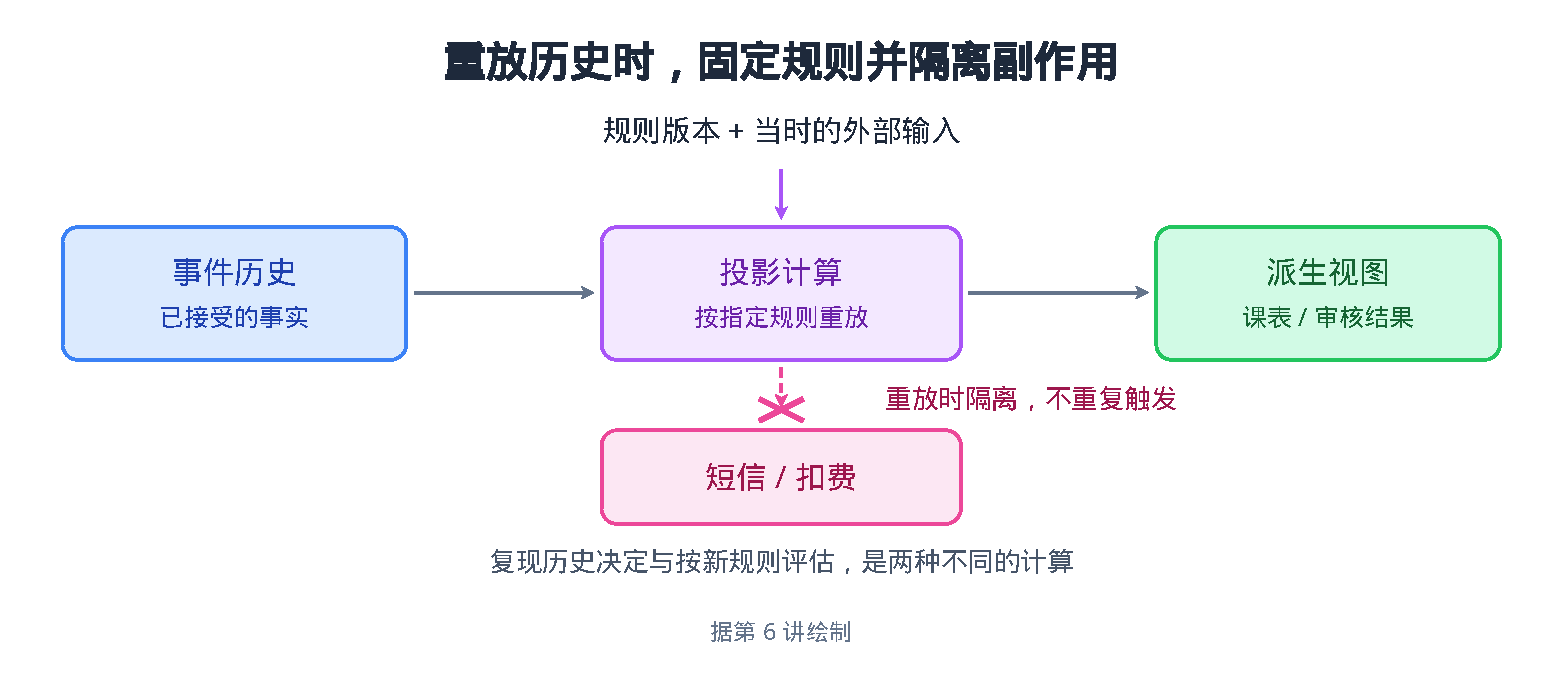
\includegraphics[width=\linewidth]{assets/mechanism.pdf}

\caption{重放历史时，固定规则并隔离副作用（据本讲绘制）}

\end{figure}

\begin{knowledgebox}{读图：机制与适用边界}

事件序列进入投影计算，规则版本和记录的外部输入一起决定派生视图。重放路径只重建结果，不再次触发短信或扣费；新业务执行的副作用走独立入口。

按旧规则复现历史决定和按新规则重新评估是不同问题。只保存事件、不保存规则依据或外部输入，无法自动保证两种结果都正确。

\end{knowledgebox}

\needspace{8\baselineskip}\section{第一章 代码便宜以后，什么成为了真正的杠杆？}

在上一讲中，我们探讨了从意图到规约再到实现的跨越，看到软件制品之间如何结成错综复杂的数据依赖网络。当今天的智能体（AI Agent）能够调用工具、修改代码、运行测试，甚至让多个智能体并行产出实现与形式化证明时，目标明确的代码编写变得前所未有地便宜。但写得出代码之后，软件工程依然困难：我们究竟要做什么？应该怎样组织系统才能承受下一次需求变化？本章将从“软件不软”这一朴素事实出发，剖析为什么当编码成本暴跌时，需求、产品设计与软件架构反而成为了决定系统成败与防止劣质代码堆积的真正杠杆。

\subsection{从意图到实现的鸿沟与对齐尝试}

在进入本讲关于需求与架构的讨论之前，我们需要先接续上一讲建立的软件生命周期视角。为什么软件开发不能像简单的流水线那样一蹴而就？当客户脑海中的模糊想法一步步走向可执行的代码时，中间究竟横亘着怎样的结构性阻碍，又是什么机制让后期的修改代价高昂？

\begin{figure}[H]\centering

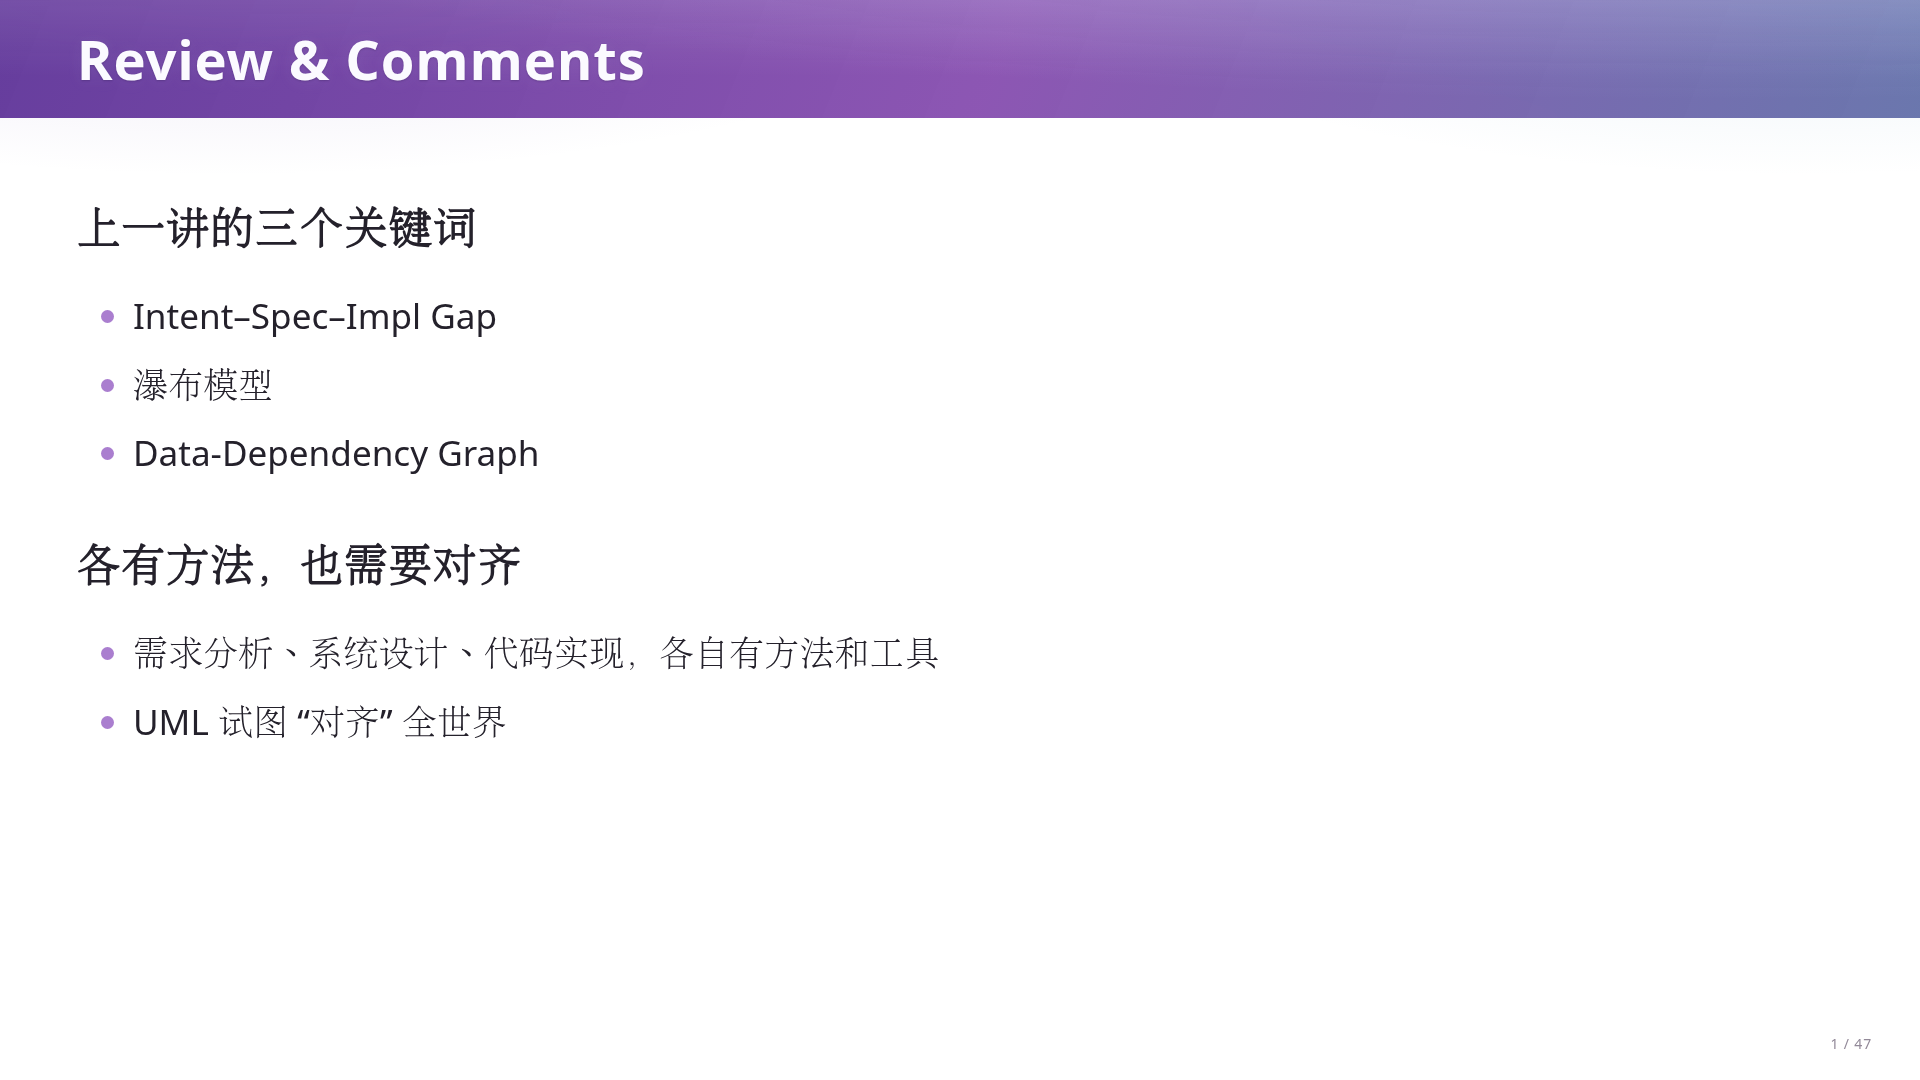
\includegraphics[width=\linewidth]{slides-images/slide-001.png}

\caption{从意图到实现的鸿沟与对齐尝试（官方课件第 1 页）}

\end{figure}

课件第一页回顾了上一讲的三个核心概念：

\begin{itemize}
\item \textbf{意图—规约—实现鸿沟}（Intent–Spec–Impl Gap，即客户主观想法、精确需求说明与最终代码实现之间的落差）、

\item \textbf{瀑布模型}（Waterfall Model，按需求、设计、实现、测试自上而下顺序推进的开发过程模型），

\item 以及\textbf{数据依赖图}（Data-Dependency Graph，描述需求、设计、模块、函数与测试用例等软件制品之间直接或间接依赖关系的网络）。

\end{itemize}
同时指出，需求分析、系统设计、代码实现各自拥有独立的方法与工具，而统一建模语言（UML，Unified Modeling Language，一种用标准图形符号表达软件结构与行为的建模语言）曾试图用一套共同语言把不同环节对同一件事的理解对齐。

Royce 在早期论文中批判简单按瀑布顺序开发的模式，正是因为数据依赖图的存在：需求与设计阶段的决定会向下派生出大批代码与测试；如果到后期才发现前面的需求理解有误或设计不合理，受其支配的一大片下游制品都会失效重做。为了在人与人之间对齐理解、在出错时知道某段代码或测试究竟对应过去的哪个决定，传统软件工程提出了可追踪性（Traceability，将测试用例、代码片段与上游需求或设计决定建立显式关联的能力）与 UML。但除了人与人难以对齐，软件工程的困难还有一个更底层的根源。

\subsection{基本观察：为什么说“软件不软”}

人们常把程序称为“软件”，仿佛它比硬件更容易捏造和修改。然而在真实的工程实践里，修改一个已有的软件系统却往往步履维艰。我们要观察传统软件工程面对的几个朴素而顽固的事实，理解软件在逻辑层面与工程修改层面的双重刚性。

\begin{figure}[H]\centering

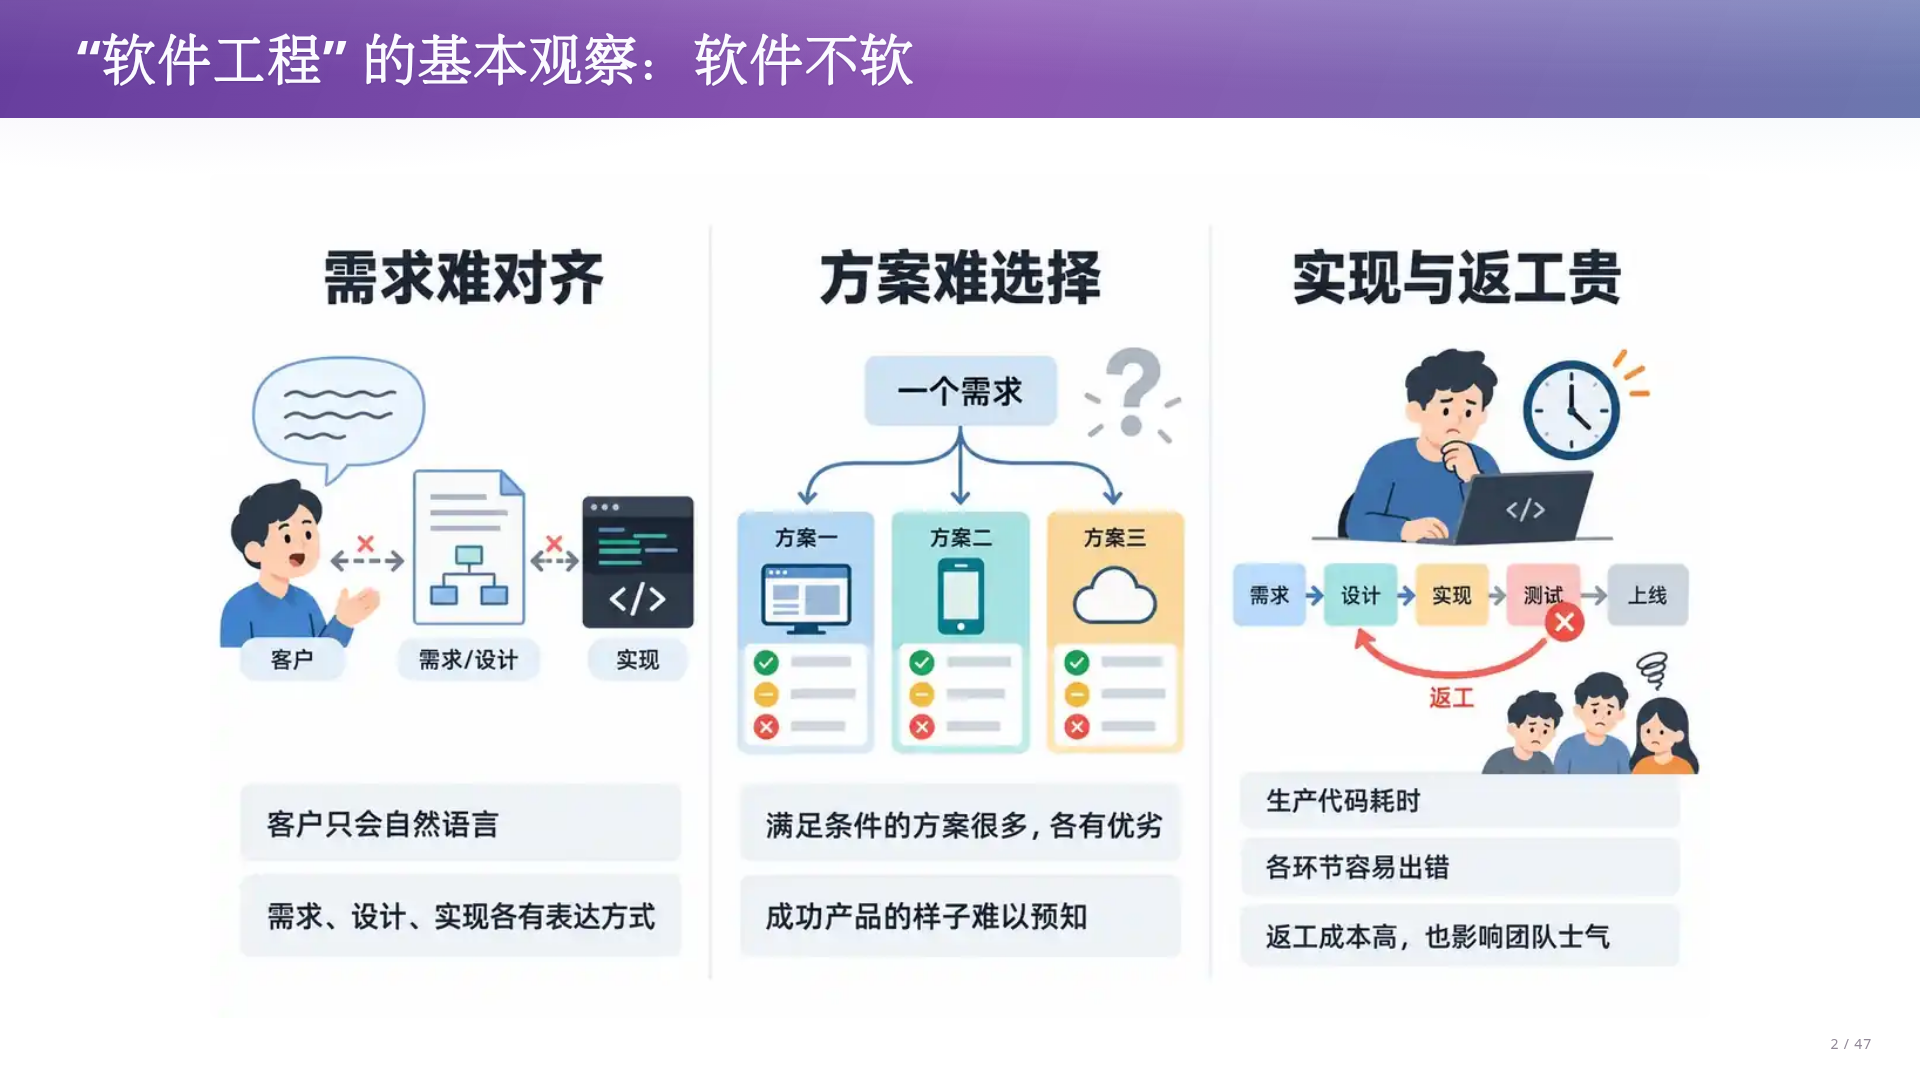
\includegraphics[width=\linewidth]{slides-images/slide-002.png}

\caption{基本观察：为什么说“软件不软”（官方课件第 2 页）}

\end{figure}

软件工程有一个基本观察：“软件不软”。围绕这一观察，软件开发长期面临三类核心困难：第一是需求难对齐，客户用自然语言描述自己的日常工作，开发者却必须将其翻译成精确无歧义的机器行为；第二是方案难选择，满足同一组要求的实现方法有很多，在性能、可维护性与开发成本上各有优劣；第三是实现与返工贵，产品真正好不好用往往要做出来才知道，而代码生产与后期返工成本极高，前面的一处误解可能演变成整个团队数周的无效劳动。

课堂提示用物理世界作了直观对比：教室里的椅背是软的、有弹性的，人靠上去会瘪下去，站起来又能弹回原状，下次还能正常使用；但软件是纯粹的逻辑制品，具有严格的形式语义（Formal Semantics，用数学方法精确定义的程序执行含义），容不下细微差错。例如程序从标准输入读取无符号整数 N（设输入 N=1）并循环读取 N 个元素到数组中，若软件运行在卫星上，宇宙射线击中内存导致表示 N 的最高位发生单比特翻转，N 就会变成巨大的数值，导致程序持续等待输入而挂起或引发内存越界崩溃。在数据中心里，先进制程处理器中电路密度极高的指令在热噪声下也可能产生静默错误（Silent Error，未触发硬件报警却算出错误结果的故障），使同一条指令在两台机器上结果不同。逻辑上的零容忍与依赖网络上的连锁反应，共同造就了“软件不软”的处境。

\subsection{软件工程方法与定量研究的困境}

既然直接写代码和返工如此昂贵，人们自然发明了各种软件工程方法，试图规范怎样访谈客户、怎样建模、怎样划分模块和安排开发过程。但为什么在高校的计算机与软件工程院系里，关于需求、产品和架构的学术研究却显得尤为棘手？

\begin{figure}[H]\centering


\includegraphics[width=\linewidth]{slides-images/slide-003.png}

\caption{软件工程方法与定量研究的困境（官方课件第 3 页）}

\end{figure}

软件工程方法与学术研究之间存在明显的张力。一方面，为了应对开发困难，业界与学界提出了各式各样的软件工程方法；另一方面，需求、产品和架构极难开展定量研究（Quantitative Research，通过控制变量、精确测量和统计检验来验证假设的研究方式），这也是课堂调侃“学校里的软工人都不在做软工”、许多论文转向“缺陷预测”等方向的背景。此外，课件引入了城市规划领域的棘手问题（Wicked Problems，Rittel 与 Webber 于 1973 年提出的概念，指问题定义本身取决于多方利益与价值判断、不存在单一客观最优解的社会与规划难题）：困难不仅在于“怎么测量”，更在于不同参与者连“什么算成功”都没有共识。

讲义提醒我们思考这种定量对照的困难：一个架构今天写起来很顺手，三年后业务变化时是否仍然合适？某种需求分析方法让产品获得了成功，究竟是方法本身有效，还是参与开发的团队本来就更有经验？这些问题很难像比较两个排序算法的运行时间那样，放进一个统一的对照实验里得出客观答案。学术界大量研究集中在编码与实现阶段（例如统计缺陷预测或用自然语言处理模型从数据中推导可追踪性关联），是因为这些对象更容易量化；但能够预测一些局部缺陷，并不自动意味着知道客户真正需要什么、产品应该长什么样。

\subsection{Agentic AI 时代的生产力转移与真正杠杆}

当定量研究难以覆盖的需求与架构问题遇上今天的生成式人工智能，软件工程的版图发生了剧烈移动。如果编写代码的环节被极大加速，原本隐藏在编码工作量背后的矛盾会如何暴露？什么将决定一个软件系统最终能走多远？

\begin{figure}[H]\centering

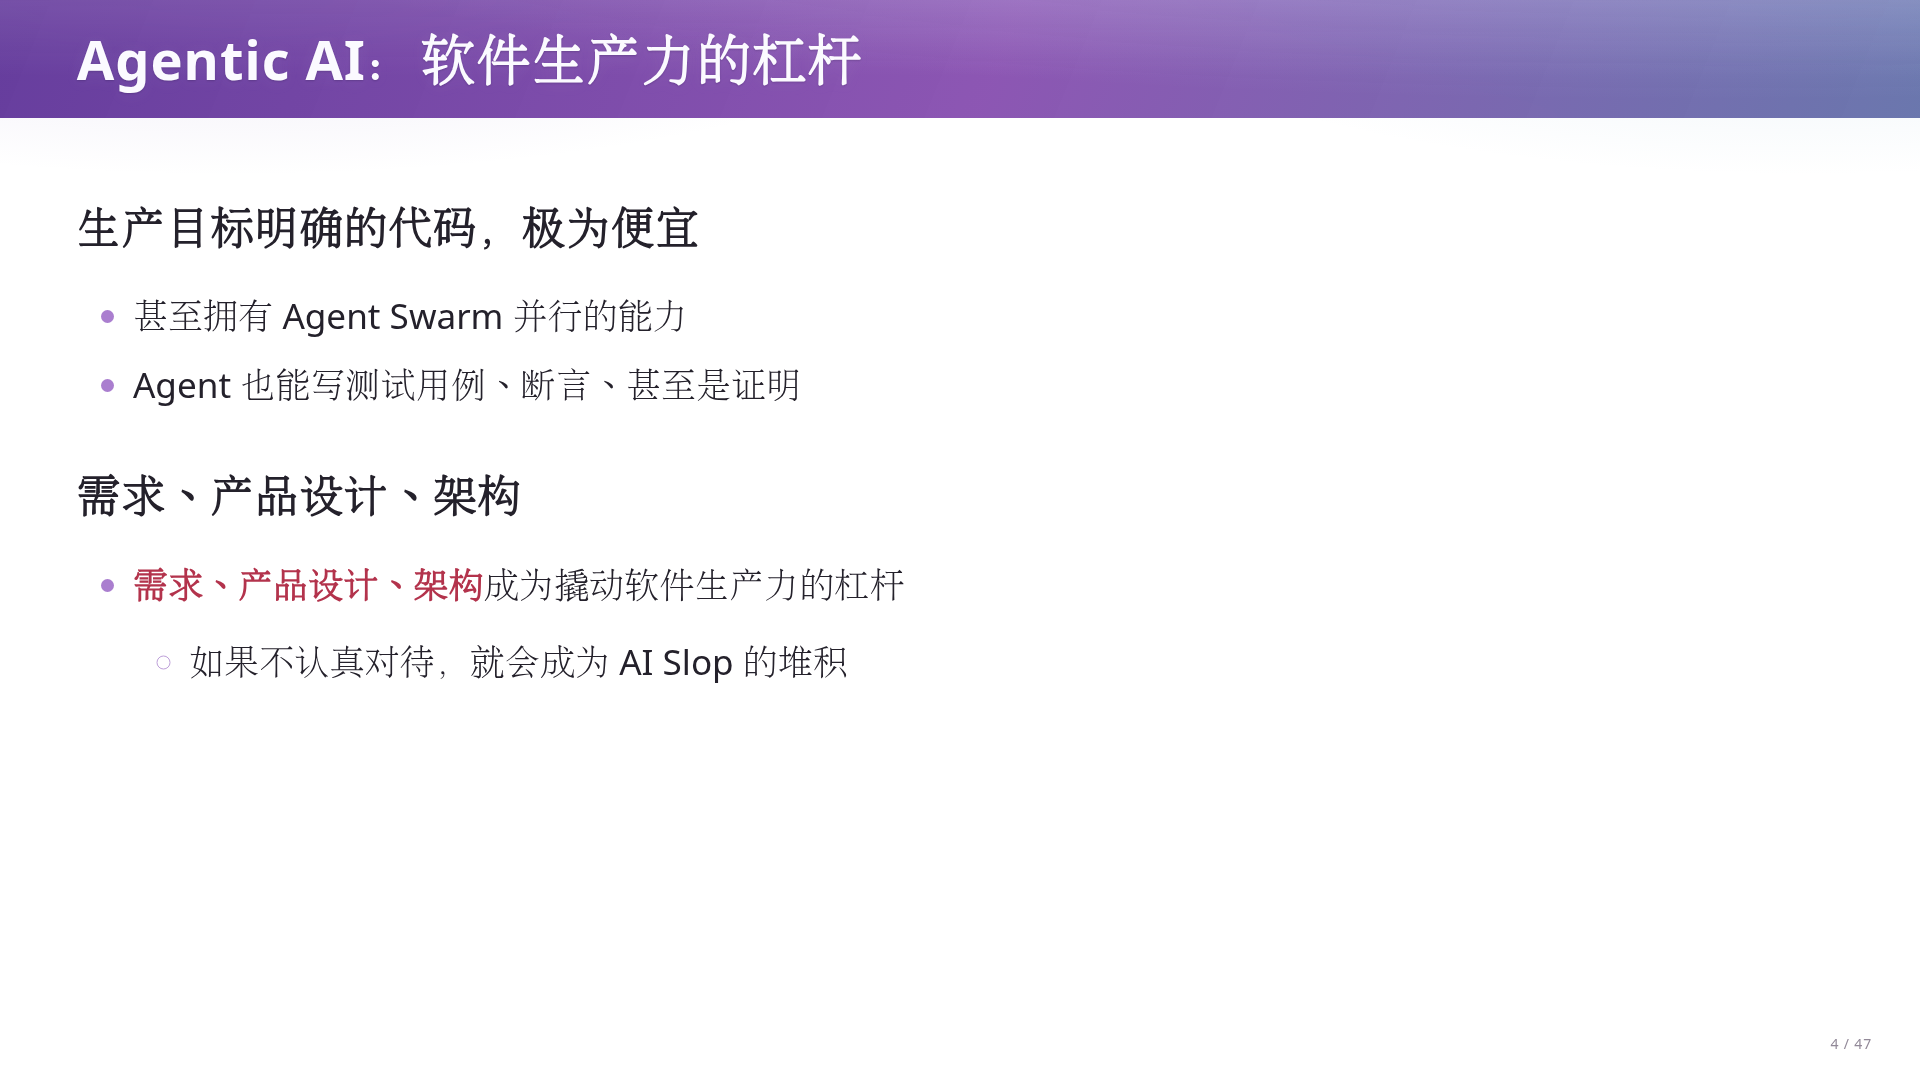
\includegraphics[width=\linewidth]{slides-images/slide-004.png}

\caption{Agentic AI 时代的生产力转移与真正杠杆（官方课件第 4 页）}

\end{figure}

智能体人工智能（Agentic AI，能够自主调用外部工具、读写代码库、执行测试并根据反馈迭代的 AI 系统）正在重塑软件开发的生产力结构：当目标足够明确时，生产代码变得极为便宜，甚至可以驱动智能体群（Agent Swarm，多个 AI 智能体并行协作完成子任务的执行模式）同时生成功能实现、测试用例、程序断言乃至形式化证明。正因如此，需求、产品设计与架构成为了撬动软件生产力的真正杠杆；如果不认真对待这三个环节，极速的生成能力只会让系统沦为劣质生成物（AI Slop，指由 AI 快速批量产出、缺乏清晰设计意图与可解释性的低质量代码或内容）的堆积。

在课堂演示与实验场景中，这种杠杆效应表现得淋漓尽致：同样是从零开始构建一个最小可行产品（MVP，Minimum Viable Product，仅实现最核心功能以快速验证需求的软件版本），只要在提示词（Prompt）里加上“采用客户端—服务器（Client-Server）架构”或“采用命令行界面（CLI）”这短短几个字，智能体就会生成截然不同的项目结构。前者会立即引入数据库文件（如 db.ts）与服务端状态，后者则围绕命令行解析库（如 cli.py）展开；这些早期文件一旦写下，就会进入智能体后续每一轮迭代的上下文，成为系统背负的技术债（Technical Debt，因早期权衡或含混决定而留下的、在未来修改时必须偿还的额外维护成本）。一个正确的抽象能让后续大量代码易于生成和验证，而一个含混的决定也会被 AI 迅速扩散到整个系统；此外，若不显式要求，AI 甚至可能生成完全没有日志输出的系统，给故障诊断留下隐患。

\begin{importantbox}{为什么“代码便宜”反而放大了架构与需求的权重}

在传统开发中，手写代码的高昂成本在无形中充当了缓冲器，迫使团队在动手前反复审视需求与设计。而在 Agentic AI 时代，只要边界清晰、验证得当，多个 Agent 并行生成代码与测试的成本极低。一旦缺乏清晰的需求界定与架构约束，AI 不会主动替人类权衡长期演化，而是把早期的含混假设以极高速度复制、扩散到每一个模块中，迅速制造出难以解释、难以修改的 AI Slop 与技术债。

\end{importantbox}

\begin{knowledgebox}{课堂直觉：从物理椅背到单比特翻转}

理解“软件不软”，可以把教室里受压后能回弹的物理椅背与纯粹由逻辑构成的程序做对比。程序依赖严格的形式语义运行，不仅需求变更会沿着数据依赖图引发大面积返工，底层运行环境的微小扰动也会被逻辑放大：无论是卫星内存中存储数组长度 N 的无符号整数因宇宙射线发生最高位翻转，还是数据中心高密度电路在热噪声下出现静默错误，局部的一点偏差都会直接破坏整体行为的一致性。

\end{knowledgebox}

\begin{warningbox}{切勿因研究局限或 AI 提效而轻视工程基础}

剖析软件工程问题时需警惕两个极端误区：第一，指出“需求与架构难以做定量对照实验”，绝不意味着 UML、可追踪性（Traceability）等软件工程方法毫无价值，它们依然承载着对齐多方人类理解的重要工程智慧；第二，不能因为 AI 能生成代码就认为程序员无需理解底层实现——没有亲手编写代码、阅读日志和体会开发痛苦的一手经验，就无法判断一项需求的实现成本与可行性，也无法做出合格的产品与架构决策。

\end{warningbox}

\par\needspace{5\baselineskip}\textbf{术语消化：第一章核心软件工程概念与生产力机制对照}

\begin{center}\small\begin{tabularx}{\linewidth}{YYY}

\toprule

术语 & 解决的问题 & 机制与课程关系\\\midrule

意图—规约—实现鸿沟（Intent–Spec–Impl Gap） & 刻画客户主观想法到精确说明再到可执行代码之间的失真 & 将自然语言转化为形式语义的过程中存在多级翻译，任何一级的偏差都会通过数据依赖图向下游放大\\[3pt]

数据依赖图（Data-Dependency Graph） & 揭示软件制品之间牵一发而动全身的耦合网络 & 需求、设计、代码与测试之间存在有向依赖，上游假设一旦变更或出错，所有依赖它的下游结论与实现均面临失效\\[3pt]

可追踪性（Traceability） & 缓解多人协作中的理解偏差与变更影响定位困难 & 通过结构化编号或建模语言（如 UML），将代码片段、测试用例与上游需求点及设计决定显式关联\\[3pt]

棘手问题（Wicked Problems） & 解释为何复杂系统的需求与架构难以找到单一最优解 & 源自城市规划，指问题定义本身依赖多方参与者的利益与价值判断，连“什么算成功”都难以达成统一共识\\[3pt]

技术债与劣质生成物（Technical Debt \& AI Slop） & 警示无架构约束的高速代码生成带来的长期维护灾难 & 早期含混的架构或数据决定会持续留在智能体上下文中，导致功能不断堆积却无法解释其正确性与协作关系\\[3pt]

\bottomrule\end{tabularx}\end{center}

\needspace{7\baselineskip}\subsection{本章小结}

本章从意图、规约与实现的鸿沟出发，结合数据依赖图与形式语义，阐明了软件作为纯粹逻辑制品“一点都不软”的本质。

尽管需求、产品与架构因涉及多方价值判断（Wicked Problems）和长周期演化而极难开展定量对照实验，但在 Agentic AI 让目标明确的代码、测试与证明变得极为便宜的今天，这三者反而成为撬动软件生产力的真正杠杆。只有把控好\textbf{需求界定与架构边界}，才能避免系统沦为难以维护的 AI Slop 与技术债泥潭。

\needspace{8\baselineskip}\section{第二章 教务系统的需求泥潭与“没有银弹”}

上一章我们看到，当能够调用工具、修改代码与执行测试的 AI Agent 让目标明确的代码生产变得极其廉价时，软件工程的核心杠杆便直接落在了需求、产品设计与软件架构上。然而，一旦把目光投向真实的业务世界，哪怕是我们每天都在使用的大学教务系统，就会发现它并非几张数据表和几个网页那样简单。为什么这类现实业务软件总会陷入史诗级的需求爆炸与改一处崩一片的“焦油坑”？既然 AI 可以迅速生成可交互的最小可行产品（MVP），为什么它依然无法充当一招制胜的“银弹”？本章将深入剖析复杂业务系统的需求泥潭。

\subsection{需求工程在课堂上的转变}

在正式解剖复杂业务系统之前，我们先来看一个长期困扰高校软件工程教学的问题：为什么“需求工程”在学校课堂上曾经极难讲授？这需要从本科生接触的编程训练特征与真实商业软件交付之间的落差谈起。

\begin{figure}[H]\centering

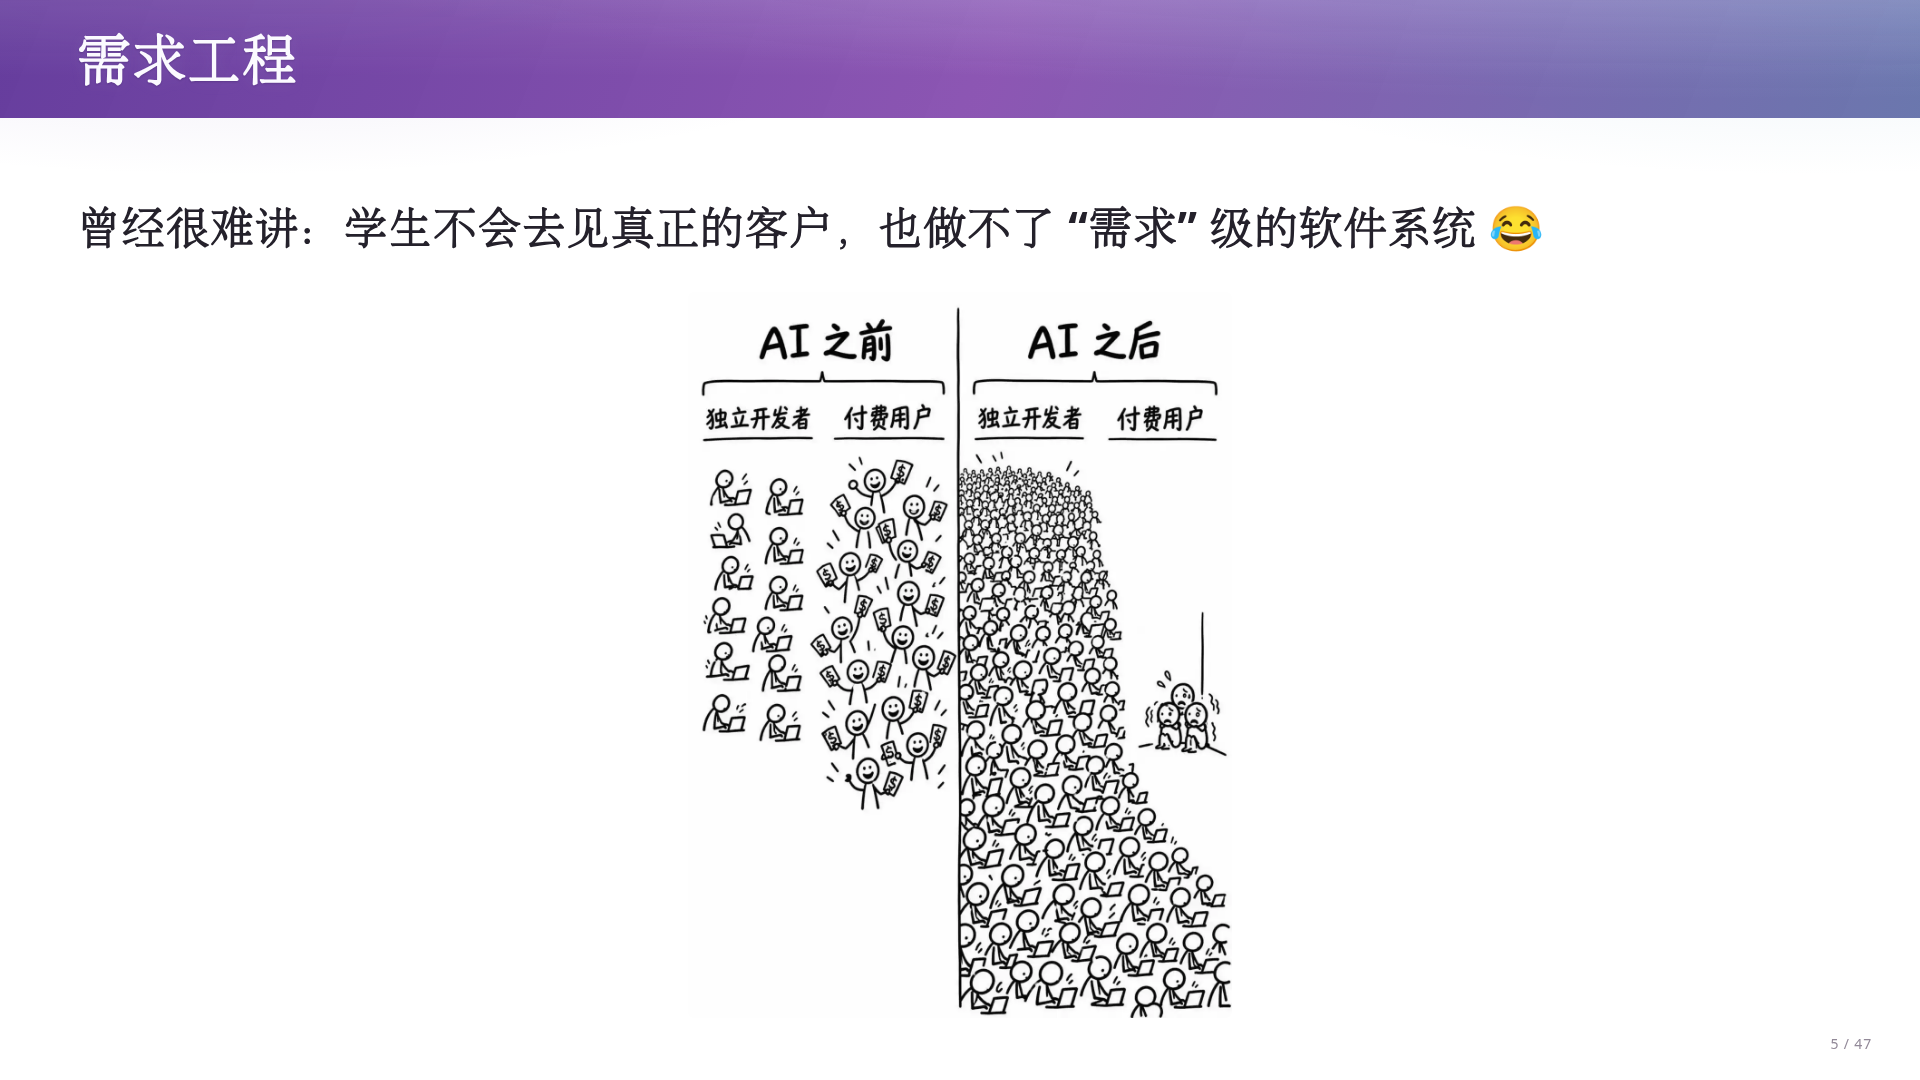
\includegraphics[width=\linewidth]{slides-images/slide-005.png}

\caption{需求工程在课堂上的转变（官方课件第 5 页）}

\end{figure}

\textbf{需求工程（Requirements Engineering）}关注如何从客户和现实业务中识别、分析、规约并管理软件系统的要求。

在传统课堂上，学生几乎没有机会接触真正的软件客户，平时完成的在线评测题目或课程小作业输入输出高度明确，规模也远未达到需要严肃处理多方需求冲突的程度。哪怕在《计算机系统基础》等课程中见过较长的实验指导书，那也是由教师预先整理好的\textbf{明确规约}，而非充满歧义的原始客户意图。

正如课堂提示所言，没有一线编码与交付的切身体验，学生不仅难以体会如何做产品经理，也不敢真的签下一份二十万元的合同去承包学校的教务系统，因为一旦逾期或达不到功能与非功能要求就无法收场。但在 AI 时代，由于构建可用原型的门槛大幅降低，每个学生都有机会从身边真实的系统出发，亲身体验一次提取需求与定义产品的过程。

\subsection{教务系统的需求爆炸与 AI 逆向提炼}

既然每个人身边都有现成的业务系统，我们不妨直接观察大学教务系统。为什么一个看似只负责选课和查成绩的网站，会演变成史诗级的需求爆炸现场？如果尝试“用魔法打败魔法”，让 AI Agent 直接调研并重做一个教务系统，会发生什么？

\begin{figure}[H]\centering


\includegraphics[width=\linewidth]{slides-images/slide-006.png}

\caption{教务系统的需求爆炸与 AI 逆向提炼（官方课件第 6 页）}

\end{figure}

观察真实的教务平台，其功能早已超出基础课表查询：不仅不断叠加自然语言问答搜索、编辑联系方式、历史授课信息、按发布时间管控的期末考试签到表打印、教材选用与大纲维护，还在疫情期间新增了慕课教学班及专门的慕课助教管理，甚至夹杂着仅在可维护时段开放的操作限制与反应迟缓的页面。面对这种需求堆积，课堂演示了让 Agent 探索教师端功能，自动提炼出一份《本科教学服务平台需求说明书》，并交由子代理直接生成可运行原型的过程。

这份由 AI 整理的需求说明书包含了业务目标、详细用例规约、功能需求目录以及对齐客户认知的术语表。讲义提醒我们，其中一项关键规范是可追踪性（Traceability），即通过有明确含义的编号，将每一个具体功能需求点与前面的角色、参与者及业务目标关联起来，从而为团队分工、进度跟踪和后续测试验证建立清晰的线索。

\subsection{从入学到毕业的全流程总需求分解}

刚才我们仅从教师端一角就看到了繁杂的功能点。如果把视角拉大到整个教务系统的生命周期，从一名新生入学到最终毕业离校，系统背后究竟串联起了哪些业务模块与底层支撑机制？这幅总需求分解图展示了主干业务流程与横切支撑能力之间的交织关系。

\begin{figure}[H]\centering

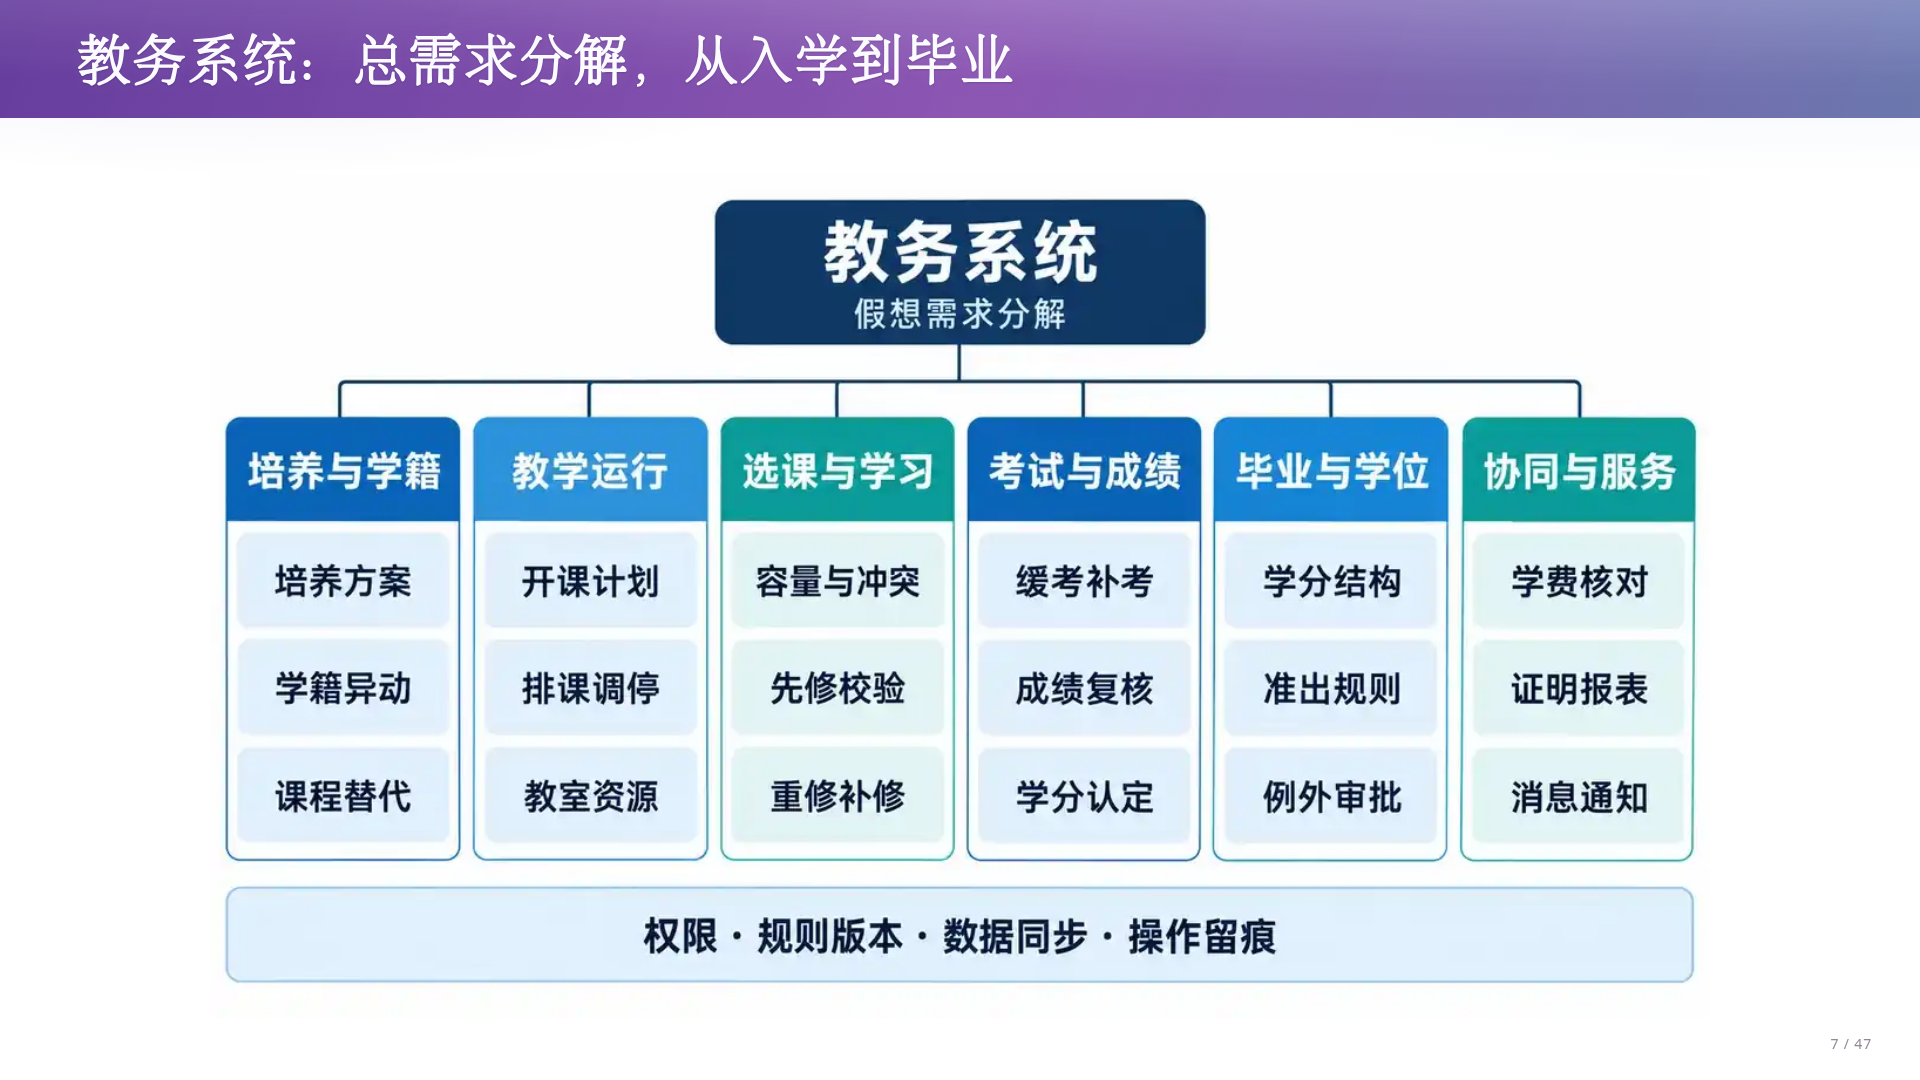
\includegraphics[width=\linewidth]{slides-images/slide-007.png}

\caption{从入学到毕业的全流程总需求分解（官方课件第 7 页）}

\end{figure}

从入学到毕业，学生主线贯穿了学籍登记、培养方案选择、选课、考试、成绩认定和毕业审核等核心环节。围绕这条主线，不同角色在同一系统上开展各自的业务：教师负责开课、管理名单与登记成绩；教务员负责排课、处理学籍异动与各类申请；教务处负责执行政策与汇总统计；财务与辅导员也各自依赖系统完成工作。在业务页面之下，系统还必须涵盖多角色身份切换、权限控制、规则管理、批次版本、数据同步与操作留痕等基础结构。

表面上看，教务系统只是浏览器里的几张表格和若干按钮，但背后却连接着诉求各异的庞大群体。课堂提示强调，做需求与产品设计必须具备同理心（Empathy）：开发者不能因为自己是熟悉命令行的极客，就假设所有用户都擅长操作复杂软件，还必须考虑例如五十三岁、临近退休、大学时代从未接触过电脑的教务员的日常界面操作习惯。

\subsection{多方利益冲突、隐含例外与棘手问题}

既然系统涉及学生、教师、教务员、教务处、财务和辅导员等众多角色，为什么不能完全照搬经典软件工程教科书的做法，把所有需求方逐一访谈一遍，汇总成一份完美无缺的需求清单后再开始写代码？这里暴露出需求工程中最棘手的两重困境。

\begin{figure}[H]\centering


\includegraphics[width=\linewidth]{slides-images/slide-008.png}

\caption{多方利益冲突、隐含例外与棘手问题（官方课件第 8 页）}

\end{figure}

第一重困境是客户往往说不清楚完整、明确的需求。每位参与者通常只熟悉自己每天处理的常规业务，很难在访谈时一次性穷举所有奇葩规则（如必修课二选一、准出规则、先修规则）和永远存在的现实例外（如转专业、交换生、缓考、补考、课程替代）。第二重困境是即便每个人都把诉求说清楚了，各方也未必能达成一致：面对同一门满员的必修课，学生希望选上课，教师希望控制班额保证教学质量，教务员则希望学生按时毕业。

这种多方利益冲突并非靠写代码就能自动消解，必须由业务方作出裁决。这正呼应了城市规划学者 Rittel 与 Webber 在 1973 年提出的棘手问题（Wicked Problems）：问题本身如何定义，直接取决于不同参与者的利益诉求与价值判断。一旦前期把某种单一假设固定成代码，后续现实世界的规则变化就会将系统拖入泥潭。

\subsection{培养方案的组合爆炸与“暗箱操作”}

为了切身感受简单业务规则如何在现实中交织成复杂网络，我们来看一个专门为教学构造的虚构案例（注意：此处的 160 学分等规定仅为课堂教学构造的假想示例，并非南京大学真实的现行教务政策）。请观察当多条局部规则同时作用于同一名学生时会发生什么。

\begin{figure}[H]\centering


\includegraphics[width=\linewidth]{slides-images/slide-009.png}

\caption{培养方案的组合爆炸与“暗箱操作”（官方课件第 9 页）}

\end{figure}

假设 2024 级李同学在 2026 年转入计算机专业，适用目标专业 2024 版方案：毕业至少需 160 学分，其中通识 40、专业必修 72、专业选修 28、实践 20，四类须分别达标；数学必修组二选一，可用 5 学分高数 A，或 4 学分高数 B 加 1 学分桥接课满足；算法课须先修数据结构，缓考生可暂选但开课前仍未通过则撤销；两门交换课获批合抵 4 学分算法课，但同一份学分不得重复计入专业选修；重修只计一次学分，成绩单保留历次记录，绩点按该假想方案规定的较高成绩计算。

单看每一条规则都不难写出判断逻辑，真正的灾难在于规则相遇与演化：转专业学生恰巧参加过交换且课程尚未认定，先修课正在等缓考成绩，选课窗口却即将关闭；或是像课堂提到的离散数学一拆为二，导致旧版准出条件与跨院系课程替代规则断裂。由于总有线下审批通过却来不及写入系统代码的特殊情况，系统最终需要提供一个记录理由、批准人和适用方案的“视为满足”兜底入口。

\subsection{数据假设扩散、直接改库与“焦油坑”}

如果软件系统在设计时没有为前面提到的线下特批和规则例外留出合法的表达空间，而学生眼看明天就要毕业审核，工程师在巨大压力下只能怎么做？这种权宜之计叠加隐式的数据假设，会将软件系统推向怎样的境地？

\begin{figure}[H]\centering

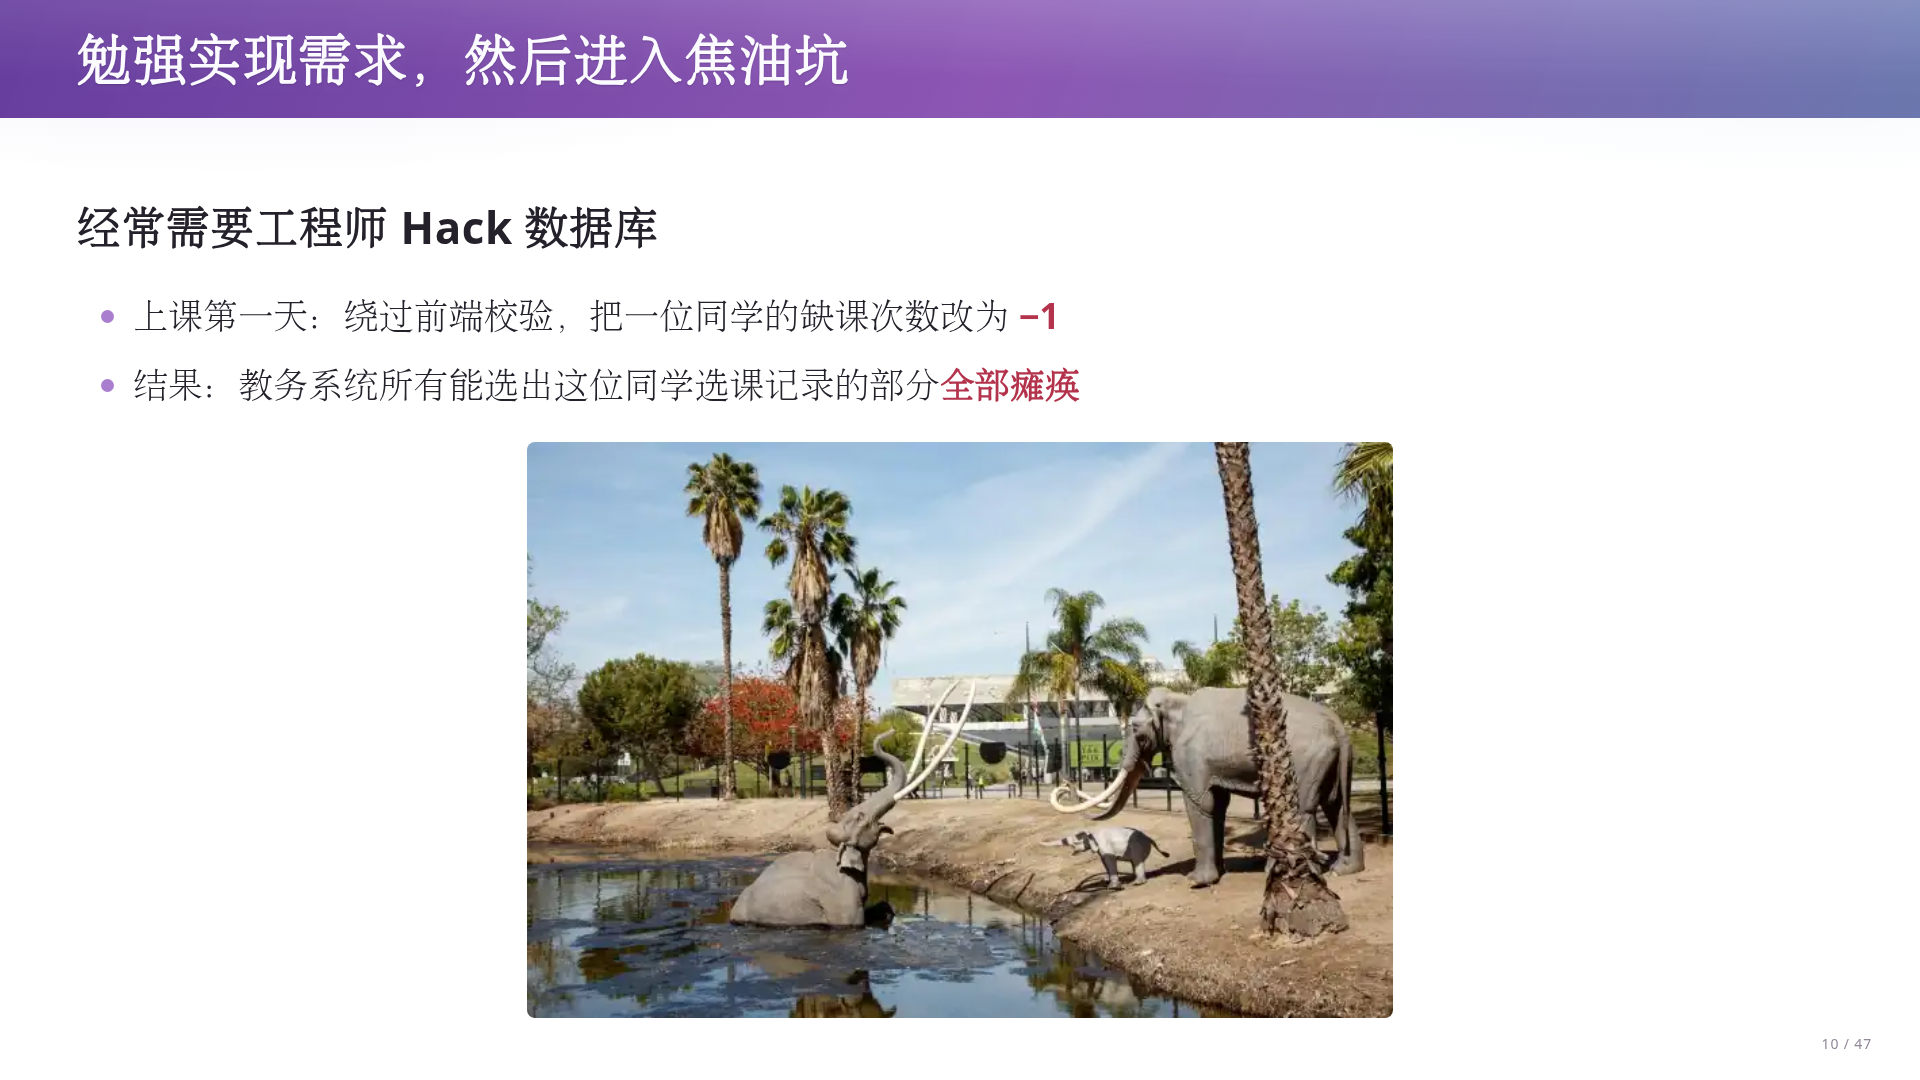
\includegraphics[width=\linewidth]{slides-images/slide-010.png}

\caption{数据假设扩散、直接改库与“焦油坑”（官方课件第 10 页）}

\end{figure}

当系统无法在业务层表达特例时，工程师往往被迫直接登录数据库修改字段（Hack 数据库），先把眼前的问题救过去。与此同时，系统内部各处代码往往暗含着未被显式声明的数据假设。课堂分享了一个 2018 年上课第一天的亲身经历：当时绕过前端网页校验，将一位同学的缺课次数从 0 改成了 -1，结果老版教务系统中所有能够查询出这位同学选课记录的页面全部瘫痪，直接返回 500 错误。

需要明确的是，我们当时只是观察到所有关联该同学选课记录的页面全部崩溃，并未据此查明或定位到数据库与后台代码中的某一处具体根因。无论这些页面是各自重复了非负假设，还是共用了一个校验或查询入口，这一现象都提示我们需要追查跨模块的数据依赖：某个看似局部的字段取值变化，可能沿着共享依赖牵动大批功能。当功能勉强凑齐、例外全靠人工补丁维持、改一处数据就顺着依赖链条影响全局时，软件就陷入了 Brooks 所说的焦油坑（Tar Pit）。

\subsection{Agentic AI 时代 MVP 的双刃剑效应}

既然传统方式容易陷入泥潭，而在 Agentic AI 时代生成代码又如此迅速，我们自然会想到敏捷开发推崇的最小可行产品（MVP）。让 AI 快速搓出一个可用的 MVP 交给客户试用，究竟能帮我们解决什么问题，又会掩盖哪些深层危机？

\begin{figure}[H]\centering


\includegraphics[width=\linewidth]{slides-images/slide-011.png}

\caption{Agentic AI 时代 MVP 的双刃剑效应（官方课件第 11 页）}

\end{figure}

最小可行产品（Minimum Viable Product，简称 MVP）主张优先实现最核心的功能，尽早把可操作的软件交给用户。这在 AI 时代变得前所未有地容易，也确实极具价值：用户面对抽象文档时想不起例外，但一看到真实的课表、选课按钮和毕业审核结果，就会立刻指出“这门课我在交换时修过了，为什么系统还让我重修？”——试用过程本身就在帮我们发掘尚未说出口的隐性需求，这也契合 Brooks 在 1987 年《没有银弹》中提倡的通过快速原型与迭代澄清需求的思路。

然而，MVP 的顺畅运行是一把双刃剑。第一次演示走通正常路径后，开发者极易产生“我已经完美驾驭了 AI”的错觉，却忽略了那些转专业、课程替代、规则追溯和人工豁免的阴暗角落（Dark Corners）此时根本还没有露出獠牙。更重要的是，生成 MVP 时的最初几句提示词和随手选定的单表数据结构，已经作为上下文写进了项目历史，开始悄然累积技术债（Technical Debt）。

\subsection{需求变更穿透数据依赖图与历史包袱}

为什么说 MVP 掩盖了真正的困难？让我们把时间轴往后推：当系统已经上线运行了一段时间，积累了真实的学生数据与审批记录后，业务方突然提出了一项看似合理的需求变更。这时系统会面临怎样的冲击？

\begin{figure}[H]\centering

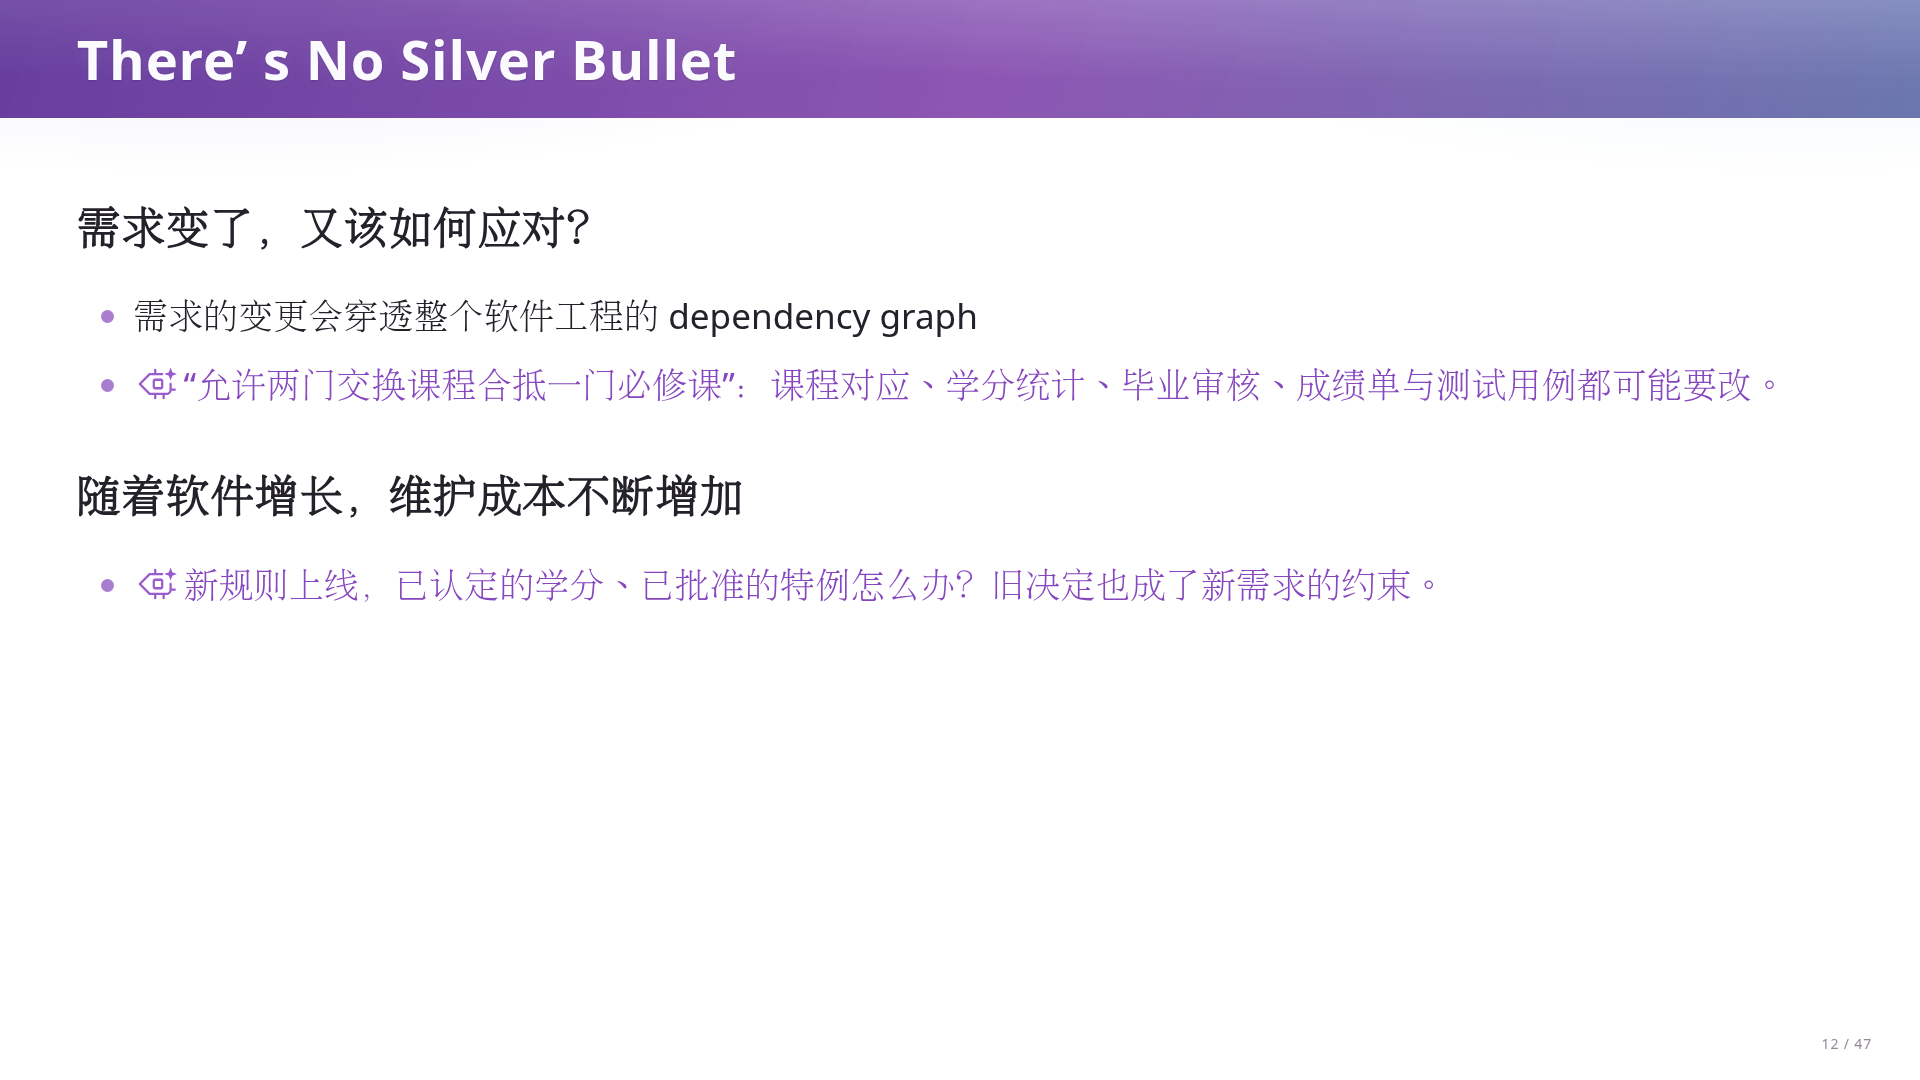
\includegraphics[width=\linewidth]{slides-images/slide-012.png}

\caption{需求变更穿透数据依赖图与历史包袱（官方课件第 12 页）}

\end{figure}

假设业务规则从原本的“一门交换课程替代一门本校课程”，变更为“允许两门交换课程合抵一门必修课”。在软件工程中，需求变更绝不只是改一个前端下拉框那样简单，它会沿着上一讲讨论过的数据依赖图（Data-Dependency Graph）穿透整个系统：课程对应关系表、学分统计逻辑、毕业审核判定、成绩单展示格式乃至配套的测试用例，全都可能被迫修改。更棘手的是，随着软件增长，过去已经发生的决定本身也变成了新需求的约束。

讲义提醒我们思考：新规则上线后，历史上已经认定过的学分要不要重新计算？过去已经批准过的特例是否继续有效？商业软件和长期运行的校务系统不像课程大作业那样可以随时清零重来，它必须背负着历史包袱与物理世界持续交互。如果最初的架构没有管理好这些数据依赖与历史依据，维护成本就会随时间呈指数级恶化。

\subsection{“没有银弹”：软件工程不存在一招制胜的万能药}

回顾从教务系统的需求泥潭到 MVP 的演进困境，我们不禁要问：无论是早年的结构化方法、面向对象、UML，还是今天能够并发编写代码的 Agentic AI，是否存在一种终极武器，能够一劳永逸地消灭软件开发中的根本困难？

\begin{figure}[H]\centering

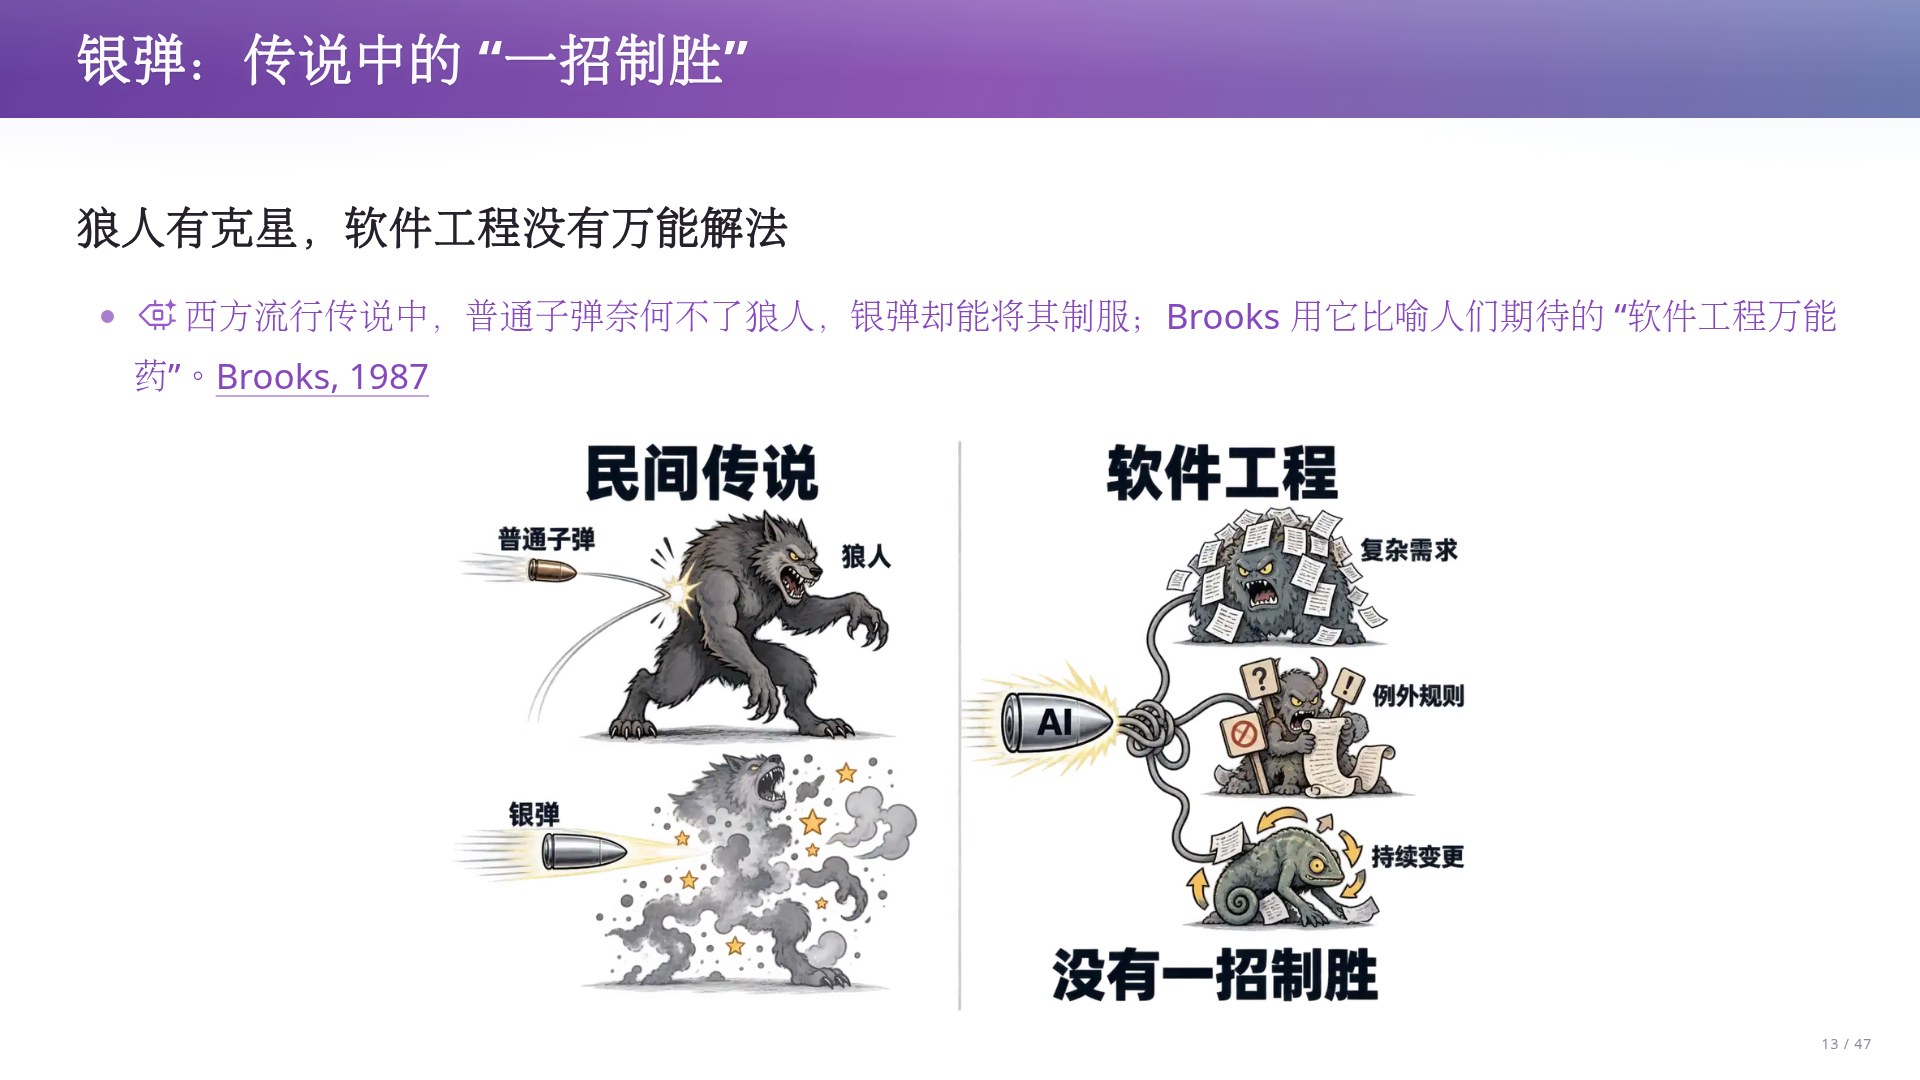
\includegraphics[width=\linewidth]{slides-images/slide-013.png}

\caption{“没有银弹”：软件工程不存在一招制胜的万能药（官方课件第 13 页）}

\end{figure}

图灵奖得主 Fred Brooks 在 1987 年发表的论文《没有银弹》（No Silver Bullet）中讨论了这一问题。在西方民间传说中，普通子弹奈何不了凶猛的狼人，只有银制的子弹（Silver Bullet）能将其制服；Brooks 借用这一典故，探讨当时未来十年内是否存在某项单一技术或管理发展，能够让软件生产力、可靠性与简明性实现数量级跃升。他在文中区分了软件的本质复杂性与偶然复杂性，说明为何单一工具难以一举消除需求与概念设计中的复杂性。

今天重读这一论断依然振聋发聩：AI Agent 确实极大地消除了编写模板代码、对齐语法细节等偶然复杂性，让快速构建原型变得轻而易举；但现实业务中的多方利益冲突、规则交织、历史包袱以及持续不断的需求变化，属于软件必须面对的本质复杂性，依然需要人来梳理和决策。既然没有银弹，我们究竟该如何安放这些复杂性？这就引出了下一章的核心主题——软件架构。

\begin{importantbox}{可追踪性（Traceability）与同理心（Empathy）}

真实软件工程面对的不是冷冰冰的评测机，而是背景各异的客户与团队。一方面，需求说明书需要通过规范的编号将每个功能点与角色、业务目标关联起来，建立可追踪性（Traceability），以便拆分任务、追踪进度并在需求变更时定位受影响的模块；另一方面，产品设计必须具备同理心（Empathy），兼顾年轻师生与不熟悉电脑操作的临近退休教务员的使用习惯，在软件中对齐真实世界的工作方式。

\end{importantbox}

\begin{knowledgebox}{为什么简单规则合在一起会变成泥潭？}

在教务系统中，单独实现“分类学分达标”“先修课检查”“缓考暂选”“交换学分冲抵”或“重修取高分”中的任何一条都不困难。真正令系统陷入泥潭的，是这些规则在同一名转专业或交换生身上同时触发时的组合爆炸，以及课程一拆为二等跨期演化。当线下特批突破了现有代码规则，系统若缺乏显式表达“由谁、因何理由、在哪版方案下视为满足”的机制，就只能沦为直接改数据库的暗箱操作。

\end{knowledgebox}

\begin{warningbox}{教学案例与生产现象的事实边界}

理解本章案例时需明确两点事实边界：第一，2024 级李同学转专业适用“毕业至少 160 学分（通识 40、专业必修 72、专业选修 28、实践 20）”及配套冲抵规则，是为教学构造的虚构案例，并非南京大学真实的现行教务政策；第二，2018 年将学生缺课次数改为 -1 导致关联选课页面全部返回 500 瘫痪，当时仅观察到外部报错现象而未查明后台代码的具体根因（多个页面失败也可能源于共享的报错入口或公共查询组件），这一经历主要启发我们关注跨模块的数据依赖。

\end{warningbox}

\par\needspace{5\baselineskip}\textbf{术语消化：第二章核心术语与概念消化表}

\begin{center}\small\begin{tabularx}{\linewidth}{YYY}

\toprule

术语 & 解决的问题 & 机制与课程关系\\\midrule

可追踪性（Traceability） & 需求、设计、代码与测试之间脱节，导致变更时无法评估影响范围、团队难以分工跟进。 & 用有明确含义的结构化编号将功能需求点与角色、业务目标、代码及测试用例关联，支撑项目管理与变更回溯。\\[3pt]

棘手问题（Wicked Problems） & 解释为什么多方参与的社会与业务系统无法靠单纯的数学优化或单次访谈得出唯一标准解。 & 源自城市规划（Rittel \& Webber, 1973），问题本身的定义取决于学生、教师、教务员等各方的利益诉求与价值判断，需由业务机制裁决。\\[3pt]

最小可行产品（MVP） & 抽象文档沟通难以激发客户说出隐含需求，且过早投入全部细节会导致返工浪费。 & 优先实现核心功能并交付可运行原型，在用户试用中暴露未说出口的例外需求，但也容易掩盖边缘规则与早期架构技术债。\\[3pt]

焦油坑（Tar Pit）与没有银弹（No Silver Bullet） & 破除“仅靠快速代码生成工具就能一劳永逸解决所有软件工程危机”的盲目乐观。 & 未管理的数据依赖与直接改库补丁会让系统陷入越挣扎越下沉的焦油坑；AI 虽降低了实现成本，但无法自动消解需求冲突与历史包袱等本质复杂性。\\[3pt]

\bottomrule\end{tabularx}\end{center}

\needspace{7\baselineskip}\subsection{本章小结}

本章以大学教务系统为切入点，剖析了现实业务软件陷入需求泥潭的根源：多角色利益冲突构成的棘手问题、培养方案与跨期变更交织出的\textbf{规则组合爆炸}，以及因缺乏合规兜底入口而被迫直接修改数据库、任由隐式数据假设沿依赖链扩散的焦油坑困境。

尽管 Agentic AI 让构建 MVP 和发掘隐性需求变得前所未有地容易，但需求变更穿透数据依赖图以及历史决定带来的约束表明，软件工程依然“没有银弹”。要真正驾驭复杂性并承接持续变化，必须依靠\textbf{恰当的软件架构}。

\needspace{8\baselineskip}\section{第三章 几行代码也有架构：从信息隐藏到十行汉诺塔}

前一章展示了最小可行产品（MVP）虽然能快速验证核心流程，却无法抵御需求变更穿透数据依赖图带来的维护泥潭。既然软件工程没有一招制胜的银弹，我们应当在项目起步阶段做些什么，才能让系统在持续变化中保持韧性？本章从软件架构的本质出发，打破“只有数据库和微服务才叫架构”的刻板印象。我们将回到 Parnas 的信息隐藏准则，剖析从命令行参数解析到十行非递归汉诺塔的四种表达，揭示选择问题表示方式如何决定复杂性的归处与系统的品味。

\subsection{软件架构的本质与信息隐藏}

面对不断膨胀的需求和不可避免的规则变更，开发者为什么不能只靠快速堆砌代码来维持系统运转？当 AI 让生成目标明确的代码变得极为便宜时，真正决定一个软件能走多远的底层因素是什么？这需要厘清软件架构的核心职责，以及它在模块边界内安放变化的基本原则。

\begin{figure}[H]\centering


\includegraphics[width=\linewidth]{slides-images/slide-014.png}

\caption{软件架构的本质与信息隐藏（官方课件第 14 页）}

\end{figure}

软件架构决定了我们如何分解问题、安排职责以及组织模块之间的依赖关系。它的首要价值在于帮助开发者\textbf{驾驭问题的复杂性}：通过简化问题表达、将复杂逻辑安放在合适的位置，并尽可能减少不必要的跨模块依赖，从而有效应对未来的需求变化、降低长期的维护成本。这种控制复杂性的设计并非大型系统的专利，哪怕再小的代码片段也存在架构决策。

早在 1972 年，David Parnas 就在关于系统模块分解的经典论文中提出了\textbf{信息隐藏}（Information Hiding，即将容易变化的设计决策封装在模块内部、仅对外暴露稳定接口的模块化设计准则）：好的模块划分应当围绕那些困难或容易变化的设计决策展开，把它们藏在边界内部，使一次需求变化尽量只影响一个局部位置。

讲义提醒我们，一个系统的品味以及它在业务演化中能走多远，很大程度上取决于早期做出的架构选择。如果在起步阶段就把所有逻辑混杂在同一个全局状态里，任何微小的外部调整都会演变成牵一发而动全身的重构。理解了信息隐藏的准则后，接下来我们将进一步审视好的架构应当呈现出怎样的结构特征。

\subsection{让复杂性有归处，让变化有边界}

当我们将 Parnas 的信息隐藏准则落实到具体的软件设计中时，应该用什么标准来判断一个架构的好坏？为什么许多表面上划分了模块或目录的系统，在遇到需求变更时依然会全面崩溃？我们可以从两个核心维度建立审视代码组织质量的标尺。

\begin{figure}[H]\centering


\includegraphics[width=\linewidth]{slides-images/slide-015.png}

\caption{让复杂性有归处，让变化有边界（官方课件第 15 页）}

\end{figure}

衡量一个软件架构是否优秀，关键看它能否做到“复杂性有归处，变化有边界”。在真实的软件工程中，业务逻辑的固有复杂性并不会凭空消失，架构的任务是为这些复杂性找到恰当的承载位置，避免它们散落到系统的各个角落。与此同时，需求的变化也必须被清晰的边界拦截在局部范围内，防止修改的波纹沿着未受控的依赖关系向整个系统扩散。

课堂提示指出，无论是单机小程序还是庞大的企业级应用，设计架构的本质都是在做解耦：想清楚哪些概念必须分开、哪些决定将来可能会变。为了证明这种架构思维不需要等到引入数据库、分布式集群或流式数据处理时才开始发挥作用，下面我们直接深入到最基础的几行 C 语言代码中一探究竟。

\subsection{小程序中的四阶段边界与语言语义约束}

在日常编写算法题或小型命令行工具时，我们是否已经在不经意间做出了架构决策？为什么课堂上严厉批判脱离设计意图的“语言律师”式教学？我们可以思考把主函数拆分为四个阶段究竟隔离了什么，以及编程语言的语法机制如何服务于软件架构。

\begin{figure}[H]\centering

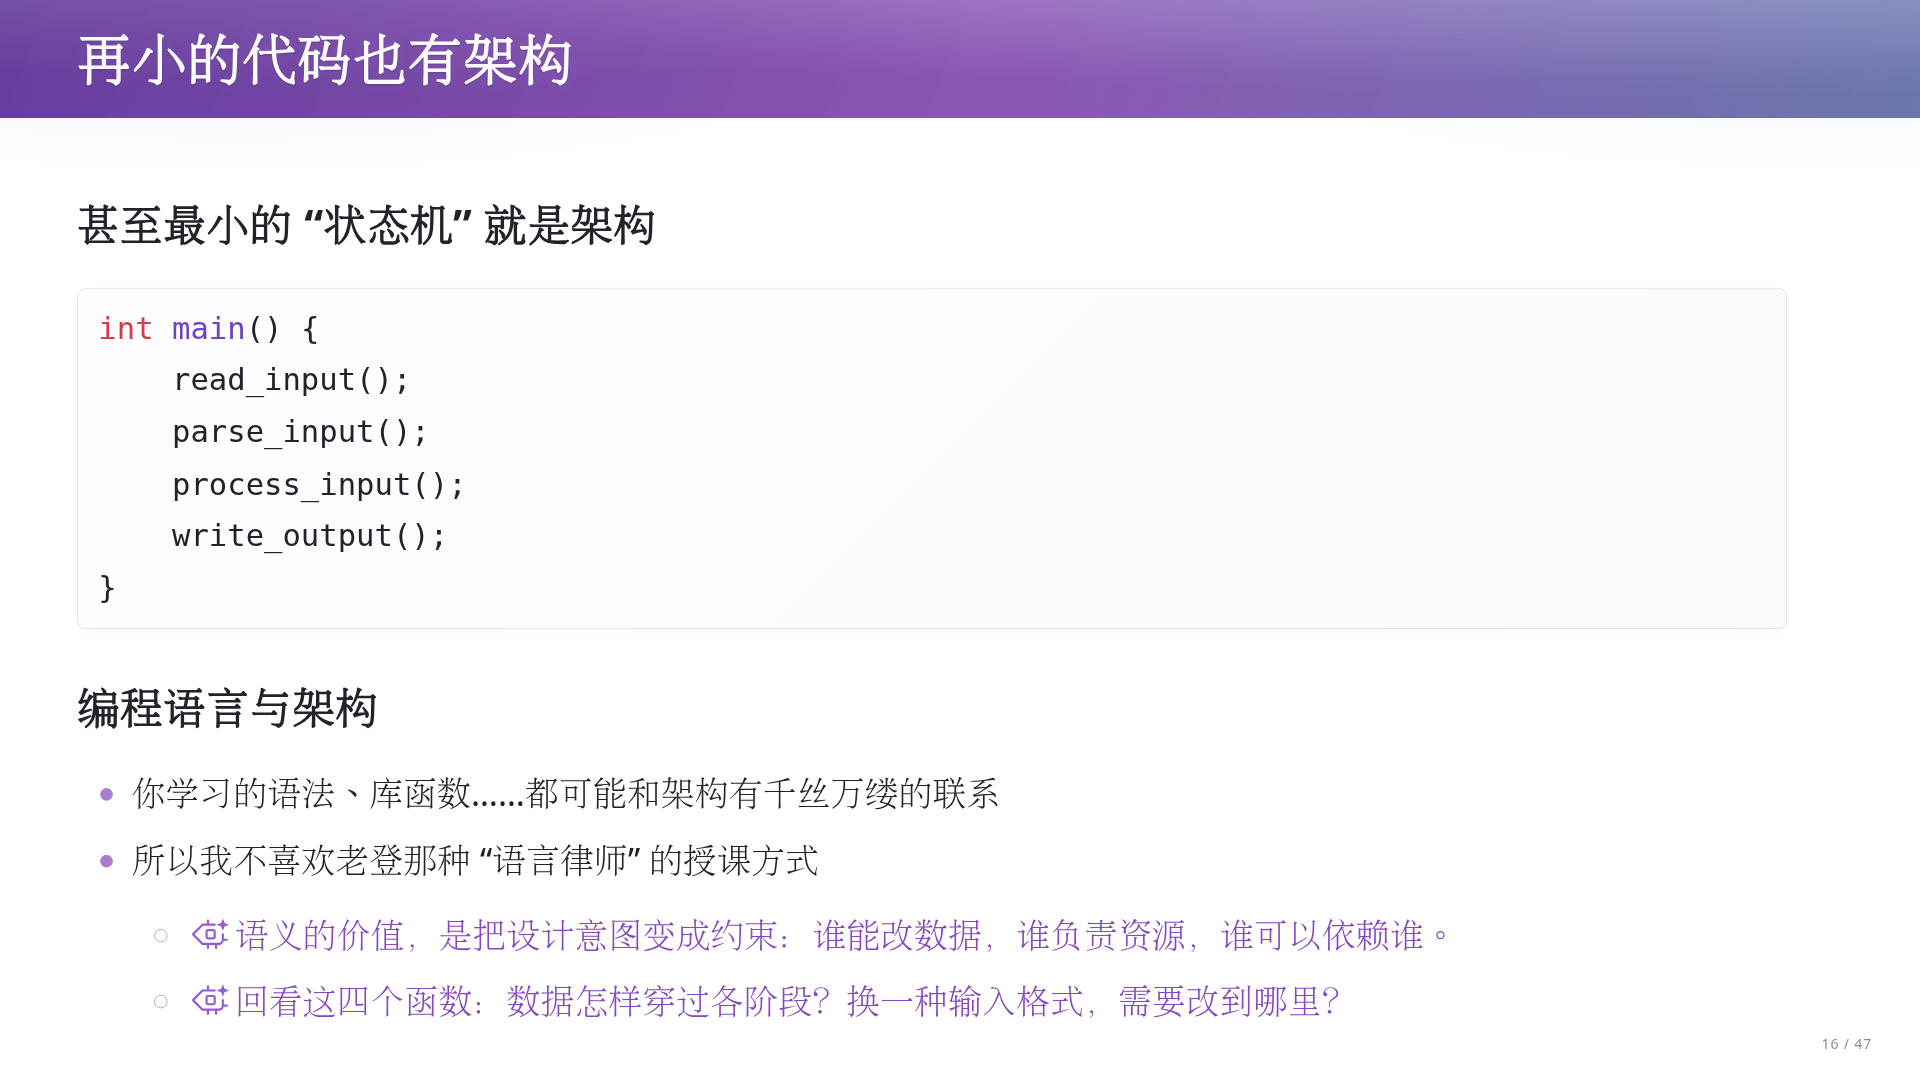
\includegraphics[width=\linewidth]{slides-images/slide-016.png}

\caption{小程序中的四阶段边界与语言语义约束（官方课件第 16 页）}

\end{figure}

哪怕是一个最小的程序，把主函数组织成 read\_input、parse\_input、process\_input 和 write\_output 四个顺序调用的阶段，本质上就是在构建一个最小的状态机架构。一旦这几个阶段成为明确的边界，我们就可以独立思考：如果更换一种输入格式，修改范围能否被限制在读取和解析阶段？核心处理算法是否必须知道结果最终是打印到终端还是写入文件？发生错误时又该由哪个环节负责？不过讲义提醒，仅仅把代码切成四个函数名，并不能自动保证边界真正存在。如果这四个函数依然在随意读写同一批全局变量，或者每一步都直接依赖其他步骤的内部数据结构细节，变化依然会四处传播。因此，学习编程语言绝不能沦为死记硬背语法边角料的“语言律师”，而要理解函数、类型、作用域与调用栈等语义构件如何把设计意图转化为硬性约束：数据怎样穿过各阶段、谁拥有并能修改状态、谁负责管理资源、谁被允许依赖谁。

在课堂口述中，老师补充了一个极具代表性的 C 语言实例：处理命令行参数 argc 和 argv。面对包含短选项、长选项乃至子命令的复杂字符串数组，如果直接用一连串字符串比较硬写，代码很快就会失控；而引入 POSIX 标准的 \texttt{getopt}（处理短选项）或 GNU 扩展的 \texttt{getopt\_long}（处理长选项），再配合顶层的子命令分发，就能把繁琐的字符串切分转化为清晰的解析状态机（通过 \texttt{while} 循环配合 \texttt{switch} 分支处理解析状态），将命令行格式的变化隔离在解析器边界之内。从几十行的参数解析再往下缩减，十行代码还能体现架构品味吗？

\subsection{十行非递归汉诺塔与问题表示的选择}

如果把代码规模压缩到极致，只看一个十行左右的基础算法问题，不同开发者和大模型之间还会产生架构层面的分野吗？为什么经典的汉诺塔问题一旦加上“不允许使用递归”的限制，许多熟练掌握语法的程序员就会突然写不出来？下面我们从认知科学与问题表示的视角重新审视这道经典题目。

\begin{figure}[H]\centering


\includegraphics[width=\linewidth]{slides-images/slide-017.png}

\caption{十行非递归汉诺塔与问题表示的选择（官方课件第 17 页）}

\end{figure}

汉诺塔问题要求将一叠大小不一的盘子从起始柱 A 借助辅助柱 B 移动到目标柱 C，约束条件是每次只能移动最上面的一个盘子，且任何时候大盘子都不能压在小盘子上面。采用递归解法时，思路非常直观：先将上面的 n - 1 个盘子搬到辅助柱，再将最大的第 n 号盘子搬到目标柱，最后把那 n - 1 个盘子从辅助柱搬到目标柱。然而当要求改为“非递归实现”时，许多人的思维就卡住了。架构关乎开发者对需求和问题本质掌控到了什么程度。认知科学研究者 Zhang 与 Norman 在 1994 年关于汉诺塔同构变体的实验中就已经观察到：同一个逻辑问题，仅仅换一种外部或内部的表示方式（Representation，即对问题状态、操作规则与约束条件的结构化编码形式），人类理解和求解它的认知难度就会发生显著改变。

课堂上老师提到，他曾用非递归汉诺塔测试保研研究生的编程能力，结果不少人摇头表示写不出。大家写不出来的根源，往往在于只盯着眼前该写哪个条件分支，却没有跳出代码去寻找更合适的表示模型。接下来，我们将依次对比 GPT-6、DeepSeek 以及教师本人给出的三种十行代码解法，看看不同的表示方式如何安放复杂性。

\subsection{第一种看法：GPT-6 的二进制数学规律}

当不加额外提示、直接要求大模型编写非递归汉诺塔时，擅长数学推理的 GPT-6 会选择怎样的架构路径？它如何绕开递归调用栈，直接算出每一步应该移动哪个盘子以及移向哪根柱子？阅读这段十行循环代码时，请注意其步号编码的前提条件、位运算规律以及背后的工程代价。

\begin{figure}[H]\centering

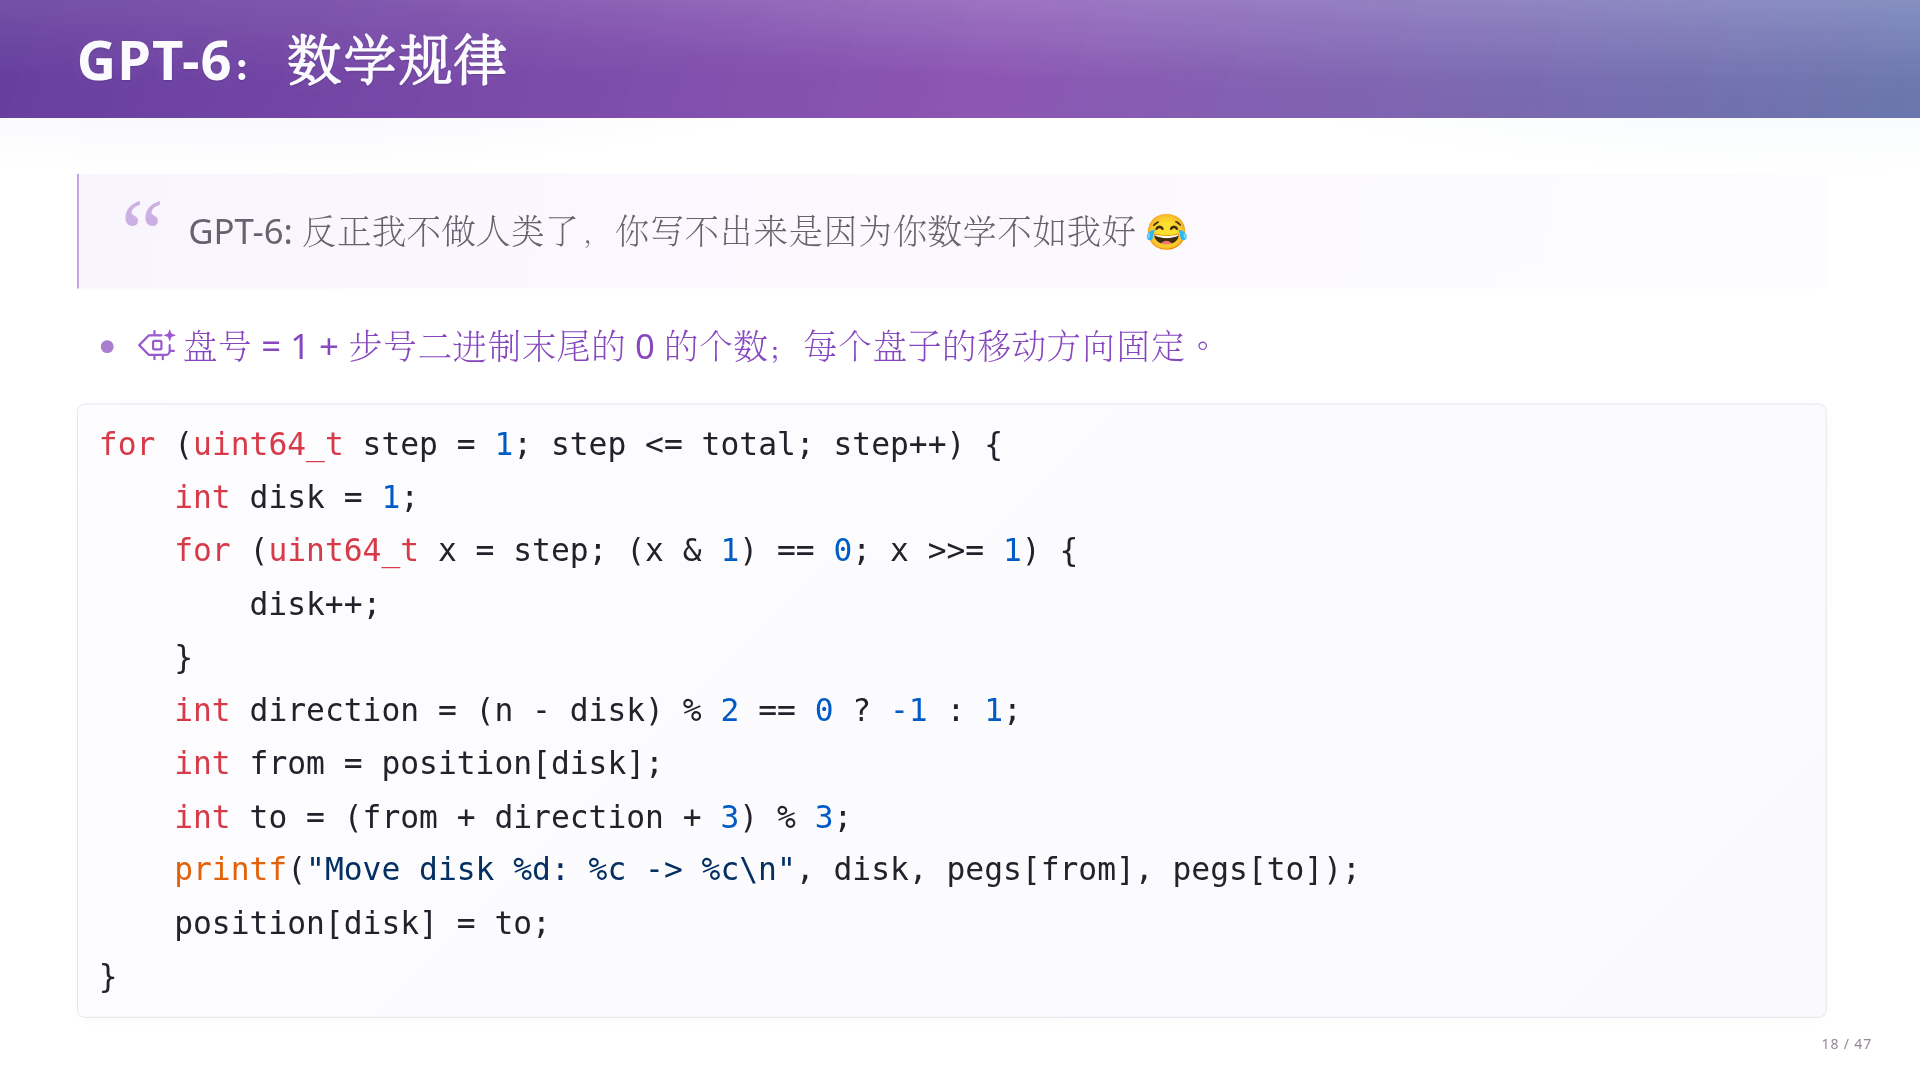
\includegraphics[width=\linewidth]{slides-images/slide-018.png}

\caption{第一种看法：GPT-6 的二进制数学规律（官方课件第 18 页）}

\end{figure}

第一种看法是抛开递归过程，直接寻找最优移动序列背后的数学规律。我们将盘子从小到大编号为 1 到 n，将最少步数解中的移动步骤从 1 开始编号。在二进制表示下，第 step 步应当移动的盘号 disk，恰好等于 step 二进制末尾连续 0 的个数加 1（代码中通过循环检查最低位 (x \& 1) == 0 并右移统计）。例如当 n = 3 时，步号 1 到 7 对应的盘号依次为 1, 2, 1, 3, 1, 2, 1。同时，每个盘子在 A、B、C 三根柱子构成的环（编码为 0、1、2，保存在字符数组 pegs 中）上移动时，其循环方向也是固定的，完全由总盘数 n 与当前盘号 disk 差值的奇偶性决定（偶数为 -1，奇数为 +1）。为了保证位移运算安全，必须严格限定 1 <= n < 64，使用 uint64\_t total = (UINT64\_C(1) << n) - 1 保存总步数，并为记录各盘当前柱号的 position 数组预留足够空间（初始全为 0）。

这段代码之所以极度紧凑，是因为开发者或模型对问题数学结构的深入理解，提前承担了原本需要由程序控制流处理的复杂性。但讲义明确指出了这种架构的代价：首先，我们必须额外解释和验证这套二进制与奇偶方向规律的正确性；其次，一旦游戏规则发生改变（例如限制某些柱子之间不能直接移动），原有的数学结构就不再适用；最后，缩短代码长度并没有消除算法固有的时间复杂度，总移动步数依然是 2\textasciicircum{}n - 1 步。

\subsection{第二种看法：DeepSeek 的显式任务栈}

如果不依赖特殊的二进制数论巧合，而是顺着人类最熟悉的任务分解思路，应该如何把递归汉诺塔改写为非递归形式？在阅读 DeepSeek 给出的这段任务栈代码时，请重点观察结构体 Task 保存了哪些状态，以及将三个子任务压入栈中时的先后顺序为什么要反过来写。

\begin{figure}[H]\centering

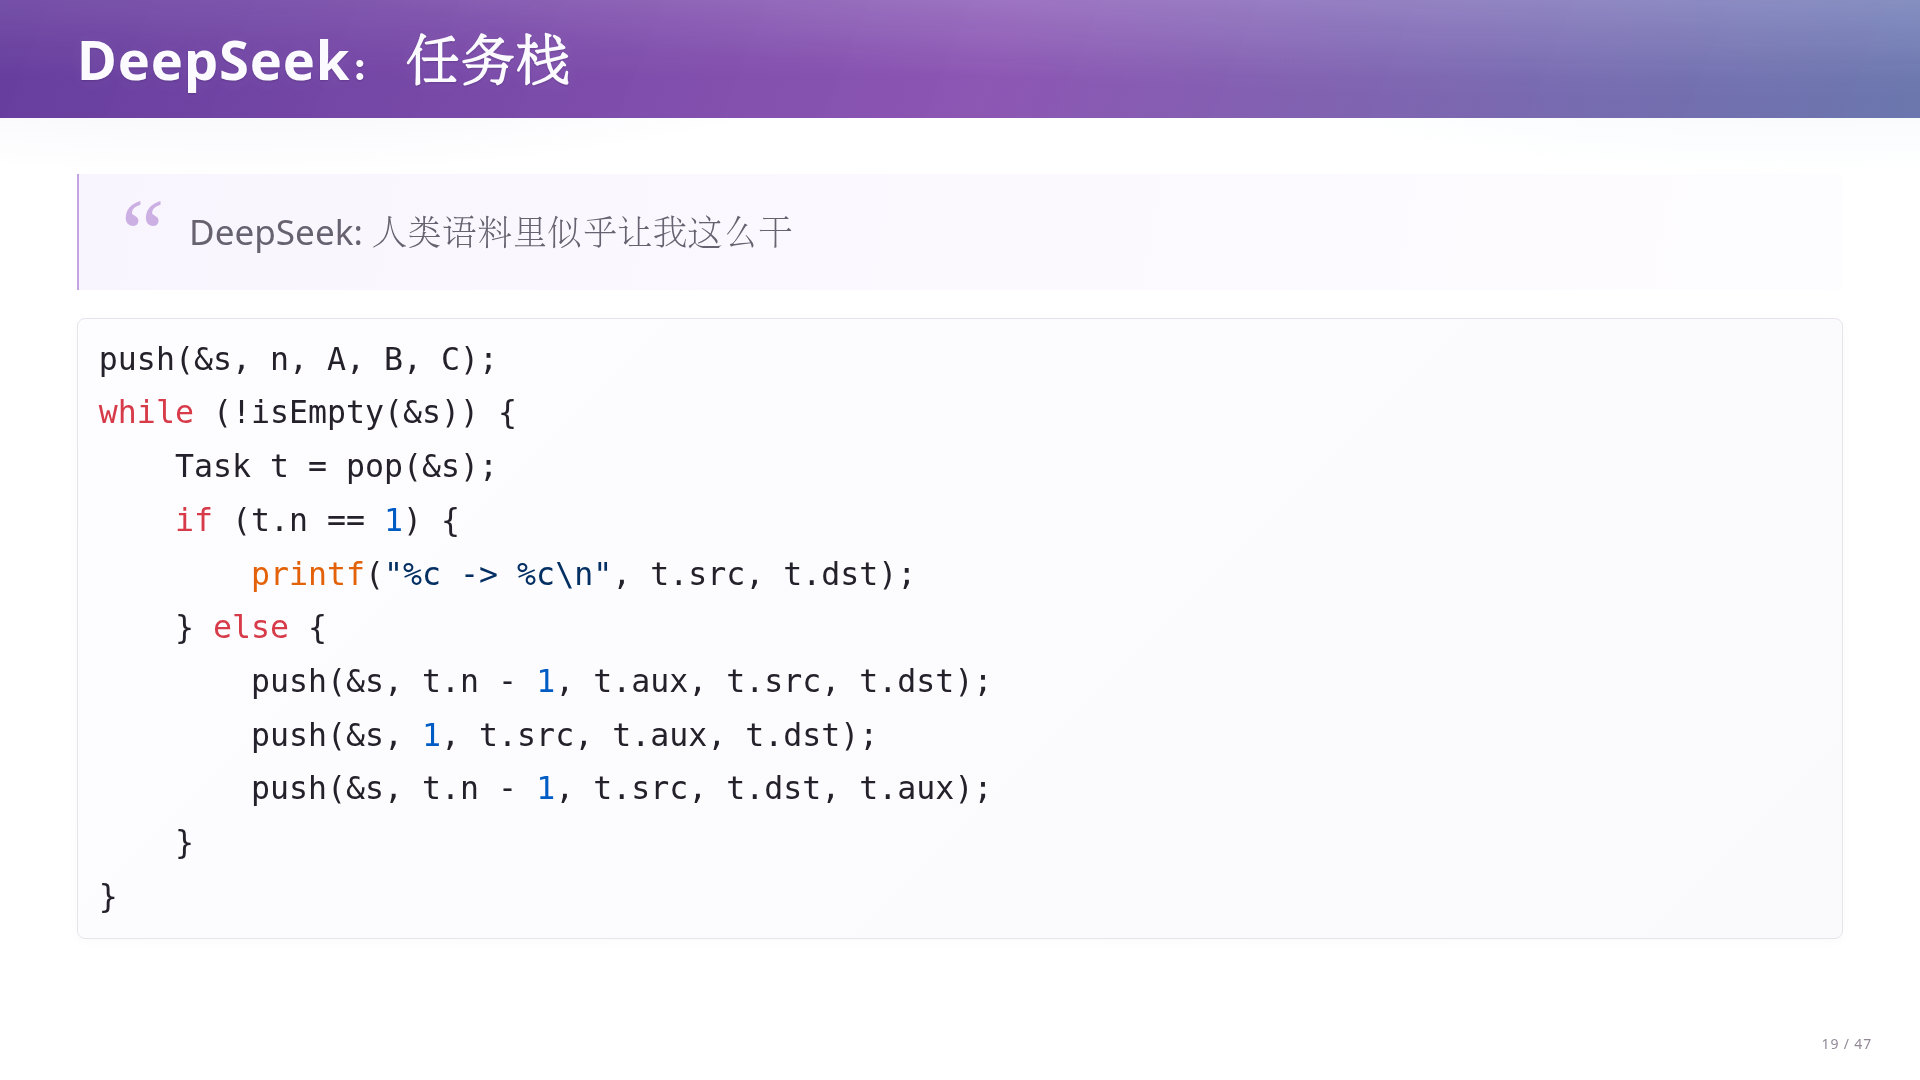
\includegraphics[width=\linewidth]{slides-images/slide-019.png}

\caption{第二种看法：DeepSeek 的显式任务栈（官方课件第 19 页）}

\end{figure}

第二种看法是把“尚未执行完的工作”显式地存放在一个任务栈中。在限定输入 \texttt{n >= 1} 的前提下，我们定义任务结构 \texttt{Task}，用来记录当前待搬运的盘子数量 \texttt{n}、起始柱 \texttt{src}、辅助柱 \texttt{aux} 和目标柱 \texttt{dst}。程序首先将初始总任务 \texttt{push(\&s, n, A, B, C)} 压入栈中，随后进入主循环：每次从栈顶弹出一个任务 \texttt{t}，如果 \texttt{t.n == 1}，就直接打印从 \texttt{t.src} 到 \texttt{t.dst} 的单步移动；如果盘数大于 1，则将该任务分解为三个子任务重新压回栈中。由于栈具有“后进先出（LIFO）”的特性，压栈顺序必须与实际业务执行的先后顺序完全相反：先压入最后执行的“将 n - 1 个盘子从 aux 移到 dst”，再压入中间执行的“将 1 个大盘子从 src 移到 dst”，最后压入最先执行的“将 n - 1 个盘子从 src 移到 aux”。

课堂上老师评价这是一种非常干净、符合人类工程直觉的架构表达。在这段代码里，原本由递归表达的任务分解结构原封不动地保留了下来，只是把隐含在系统后台的待办工作变成了由程序员显式维护的数据结构。它完全不依赖前一种解法里晦涩的步号奇偶规律，只要能把递归分解的业务意图说清楚，就能自然地写出正确的实现。

\subsection{第三种看法：基于小步操作语义的抽象机器}

如果把视角再往外推进一步：不仅要解决汉诺塔这一道题，还要寻找一种能够将任意递归函数甚至互相调用的函数机械地转化为非递归程序的通用架构，应该怎么做？阅读教师（绿导师）编写的这段代码时，请思考栈帧 Frame 中的程序计数器 pc 是如何驱动状态机一步步运转的。

\begin{figure}[H]\centering

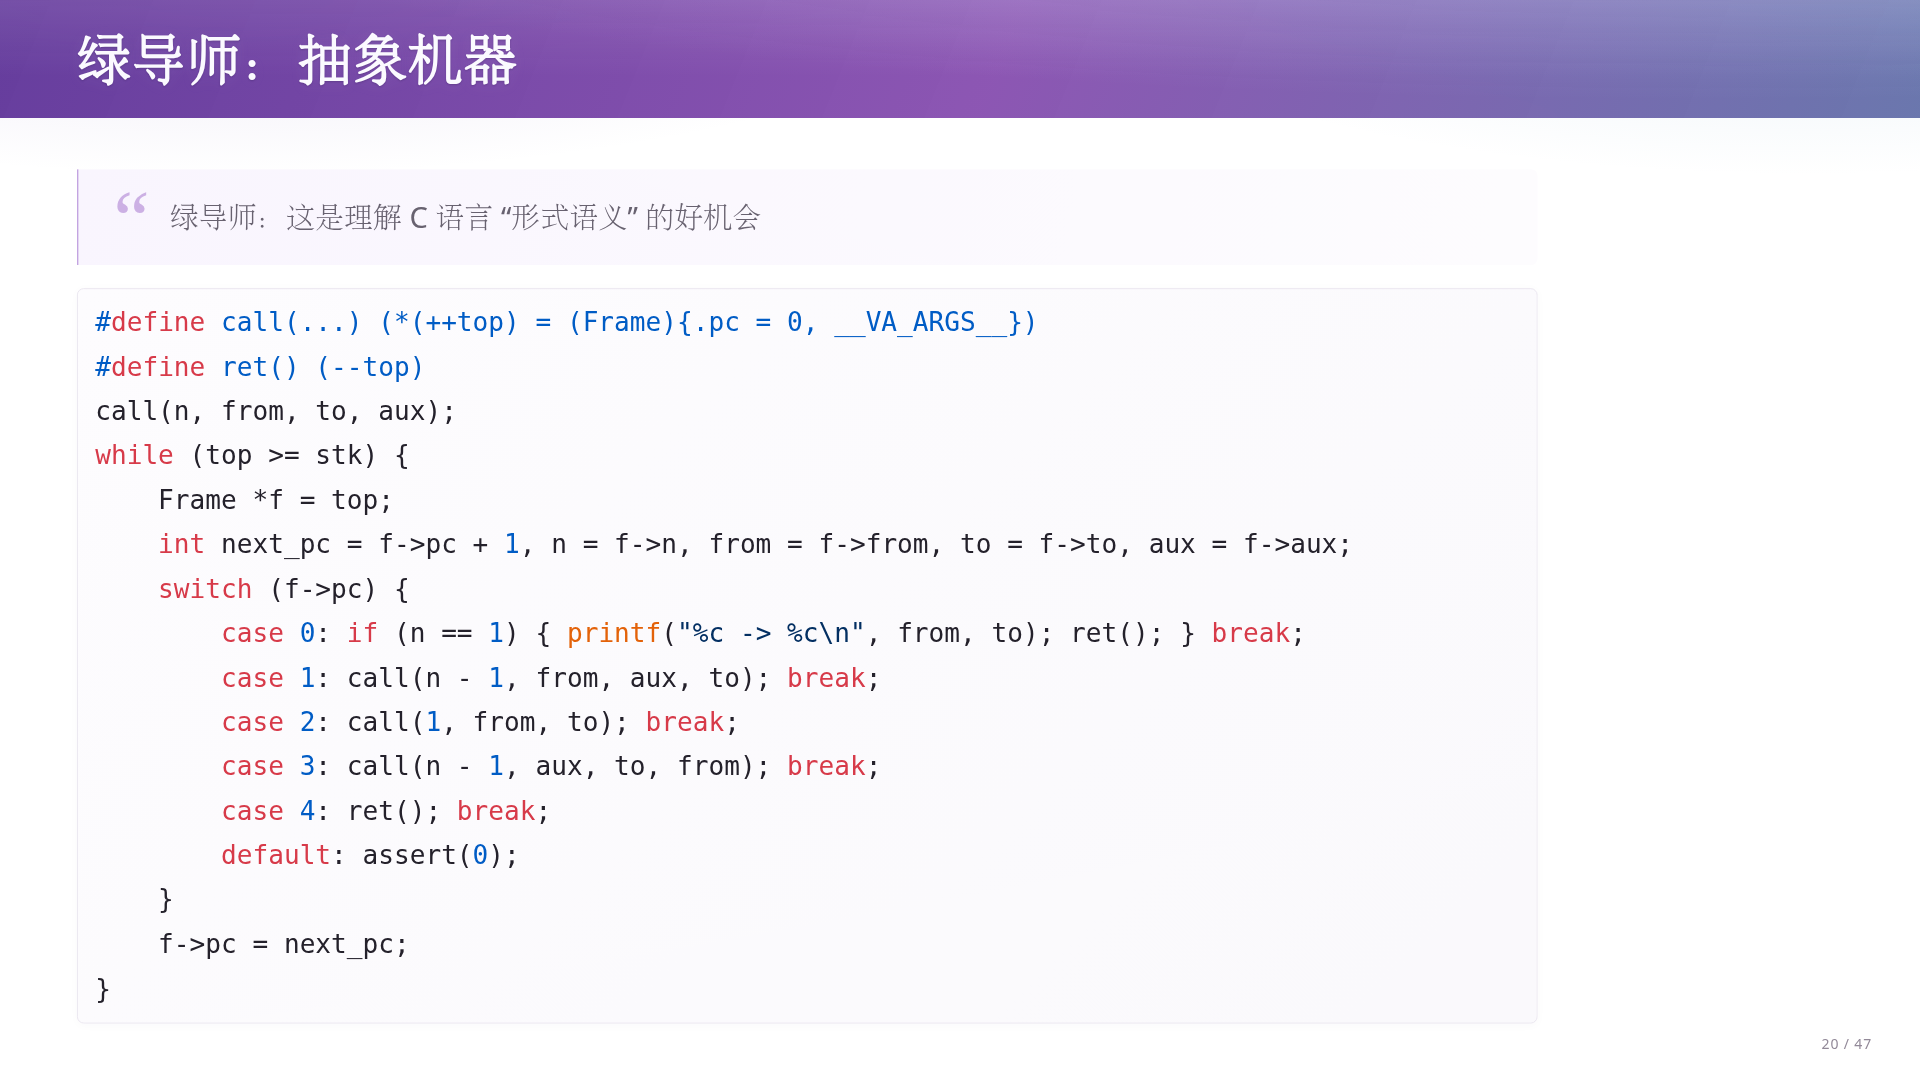
\includegraphics[width=\linewidth]{slides-images/slide-020.png}

\caption{第三种看法：基于小步操作语义的抽象机器（官方课件第 20 页）}

\end{figure}

第三种看法是直接模拟函数调用的底层执行过程，在十行代码里构造一台微型的抽象机器（Abstract Machine，用明确的数据结构显式维护调用栈帧与程序计数器、按单步状态转移规则推进程序执行的计算模型）。每一层函数调用都用一个栈帧 Frame 表示，内部保存当前层的参数 n、三根柱子的角色（from、to、aux），以及记录“当前这层函数执行到了哪一步”的程序计数器 pc。课件原图用指针 \texttt{top} 配合 \texttt{top >= stk} 和 \texttt{--top} 做了十行示意（省略了 \texttt{n >= 1} 与栈容量检查；需注意在标准 C 中，当最后一帧弹出后 \texttt{top} 指向数组首元素之前属于未定义行为，工程实现应改用整数栈深 \texttt{sp}，以 \texttt{sp > 0} 判非空、\texttt{stk[sp - 1]} 取栈顶帧）。在这台机器中，\texttt{call} 负责在栈顶压入一个 \texttt{pc} 初始化为 0 的新栈帧，\texttt{ret} 负责弹出栈顶帧。主循环在栈非空时持续运行，每次取出当前栈顶帧 \texttt{f}，先记录 \texttt{next\_pc = f->pc + 1}，再按 \texttt{f->pc} 进入 \texttt{switch} 分支：当 \texttt{pc} 为 0 时检查基线条件 \texttt{n == 1}（要求初始输入 \texttt{n >= 1}），满足则打印移动并执行 \texttt{ret()}；当 \texttt{pc} 为 1、2、3 时依次压入三次子调用；当 \texttt{pc} 为 4 时执行 \texttt{ret()} 结束本层函数；同时将 \texttt{f->pc} 推进为 \texttt{next\_pc}，使子调用返回后能接着向后执行。

老师在课堂口述中强调，这种写法源自编程语言的形式语义，特别是小步操作语义（Operational Semantics，将程序的执行严格定义为程序状态在单步规则下的离散转移过程）。在这台抽象机器眼里，函数调用与返回不再是黑盒语法，而是显式的栈帧状态转移。掌握了这套架构，哪怕遇到函数 F 调 G、G 又调 F 的复杂互递归，也能按部就班地翻译成状态机并进一步化简。

\subsection{反面教材：缺乏抽象与命名冲突的混乱实现}

如果开发者既没有发现数学规律，也没有建立任务栈或抽象机器的模型，而是直接在代码里硬凑非递归逻辑，写出来的程序会变成什么样？观察本页课件原图展示的网络博客搜索结果，看看缺乏架构抽象的代码会暴露出哪些典型的工程缺陷。

\begin{figure}[H]\centering

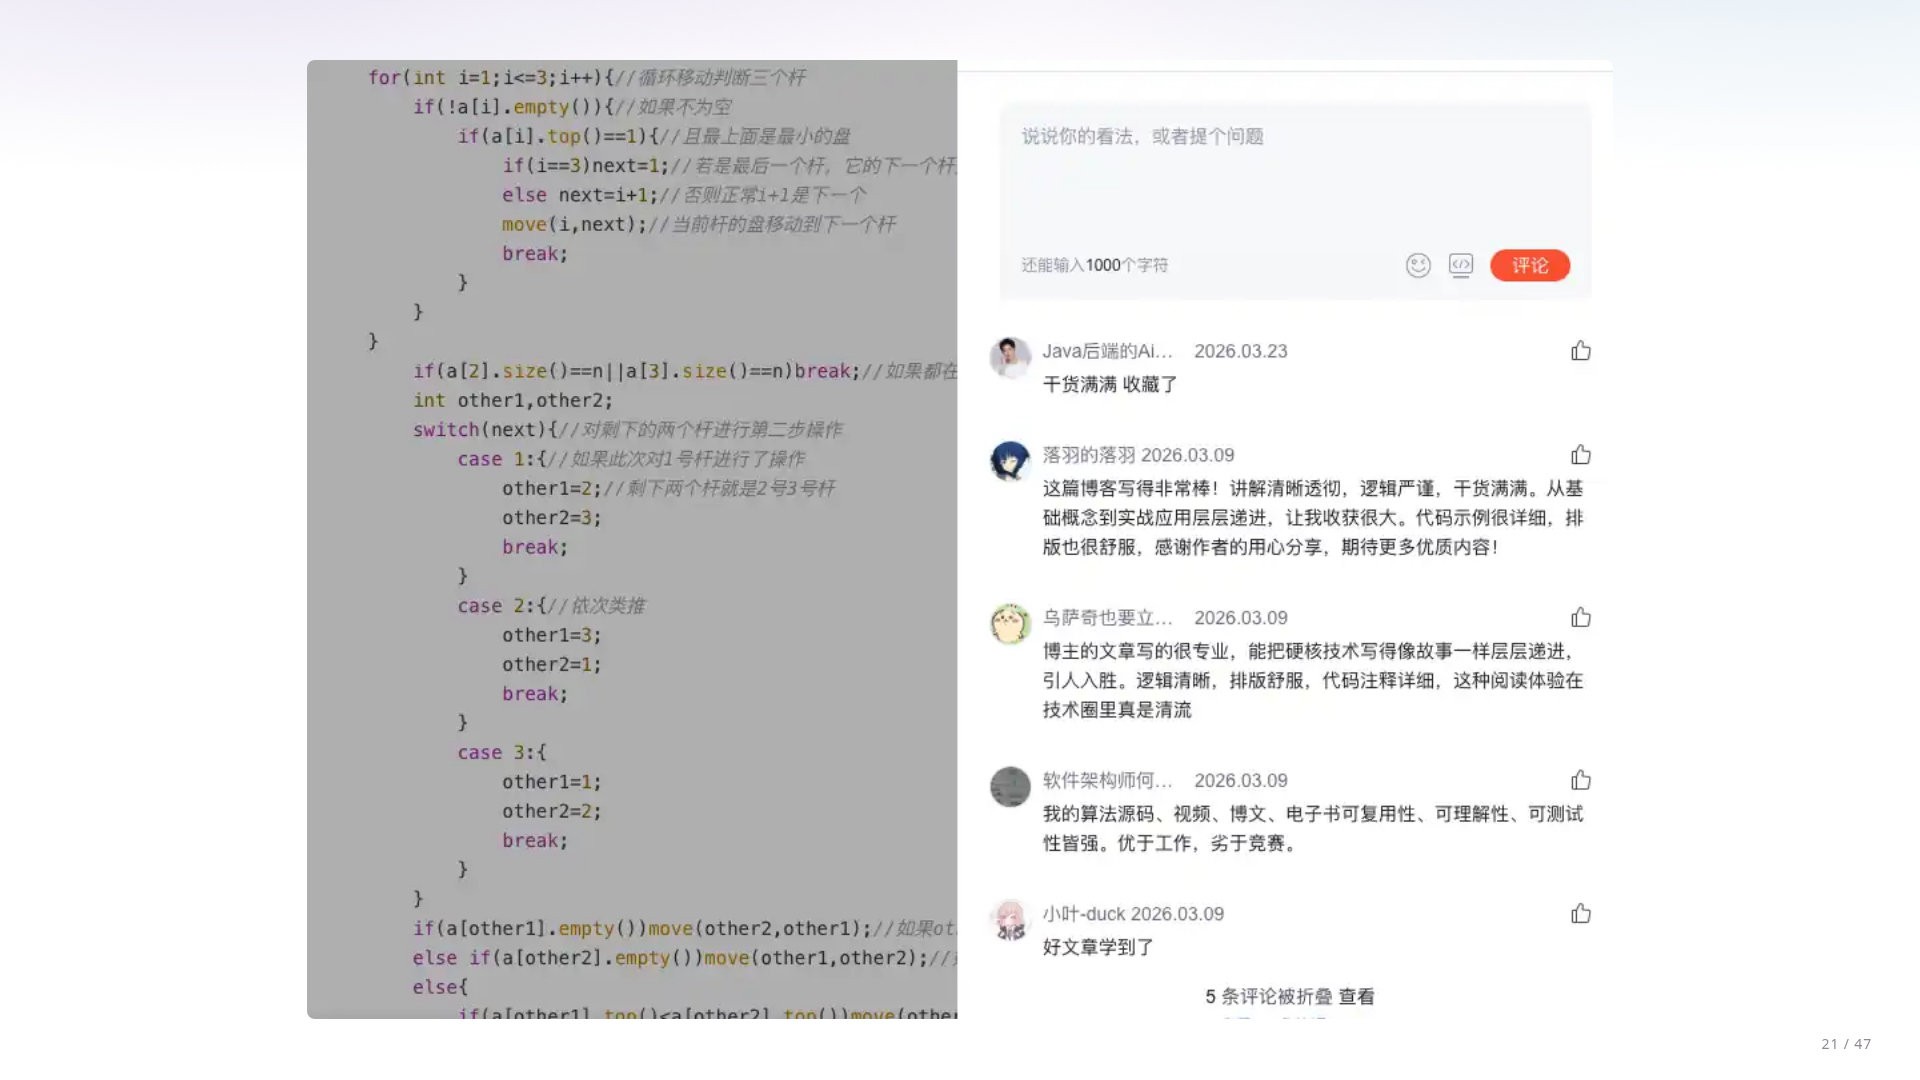
\includegraphics[width=\linewidth]{slides-images/slide-021.png}

\caption{反面教材：缺乏抽象与命名冲突的混乱实现（官方课件第 21 页）}

\end{figure}

课件原图展示了在搜索引擎中查找“非递归汉诺塔”时排名靠前的一篇技术博客代码片段。与前面三种清晰紧凑的架构表达形成鲜明对比，这段代码没有提炼出统一的任务或状态机抽象，而是试图用大量琐碎的变量、冗长的循环和层层嵌套的条件分支去修补盘子移动的细节。更糟糕的是，作者在代码中自定义了一个名为 move 的辅助函数，而在引入 C++ 标准库命名空间后，这个标识符极易与标准库中的 std::move 发生命名冲突。尽管代码冗长且设计粗糙，页面右侧的评论区却充斥着整齐划一的夸赞，营造出一种虚假的高质量假象。

课堂提示幽默地指出，如果在学习编程时被这种缺乏抽象的劣质代码（甚至比 AI 随意生成的 Slop 还要糟糕）污染了品味，还不如直接向优秀的大模型学习。这个反面案例生动地说明：当一个人只盯着眼前的局部语法分支而没有整体架构时，哪怕面对十行代码就能解决的问题，也会迅速制造出一团难以维护的乱麻。

\subsection{四种表达的对照：选择表示就是选择安放复杂性}

回顾同一个非递归汉诺塔问题的四种代码呈现，为什么短短十来行代码就能映射出如此悬殊的工程境界？在软件设计中，“选择一种表示方式”究竟意味着我们在对系统的复杂性和未来的变化做什么样的承诺？通过将这四种表达并列对照，我们可以总结十行代码背后的架构选择。

\begin{figure}[H]\centering

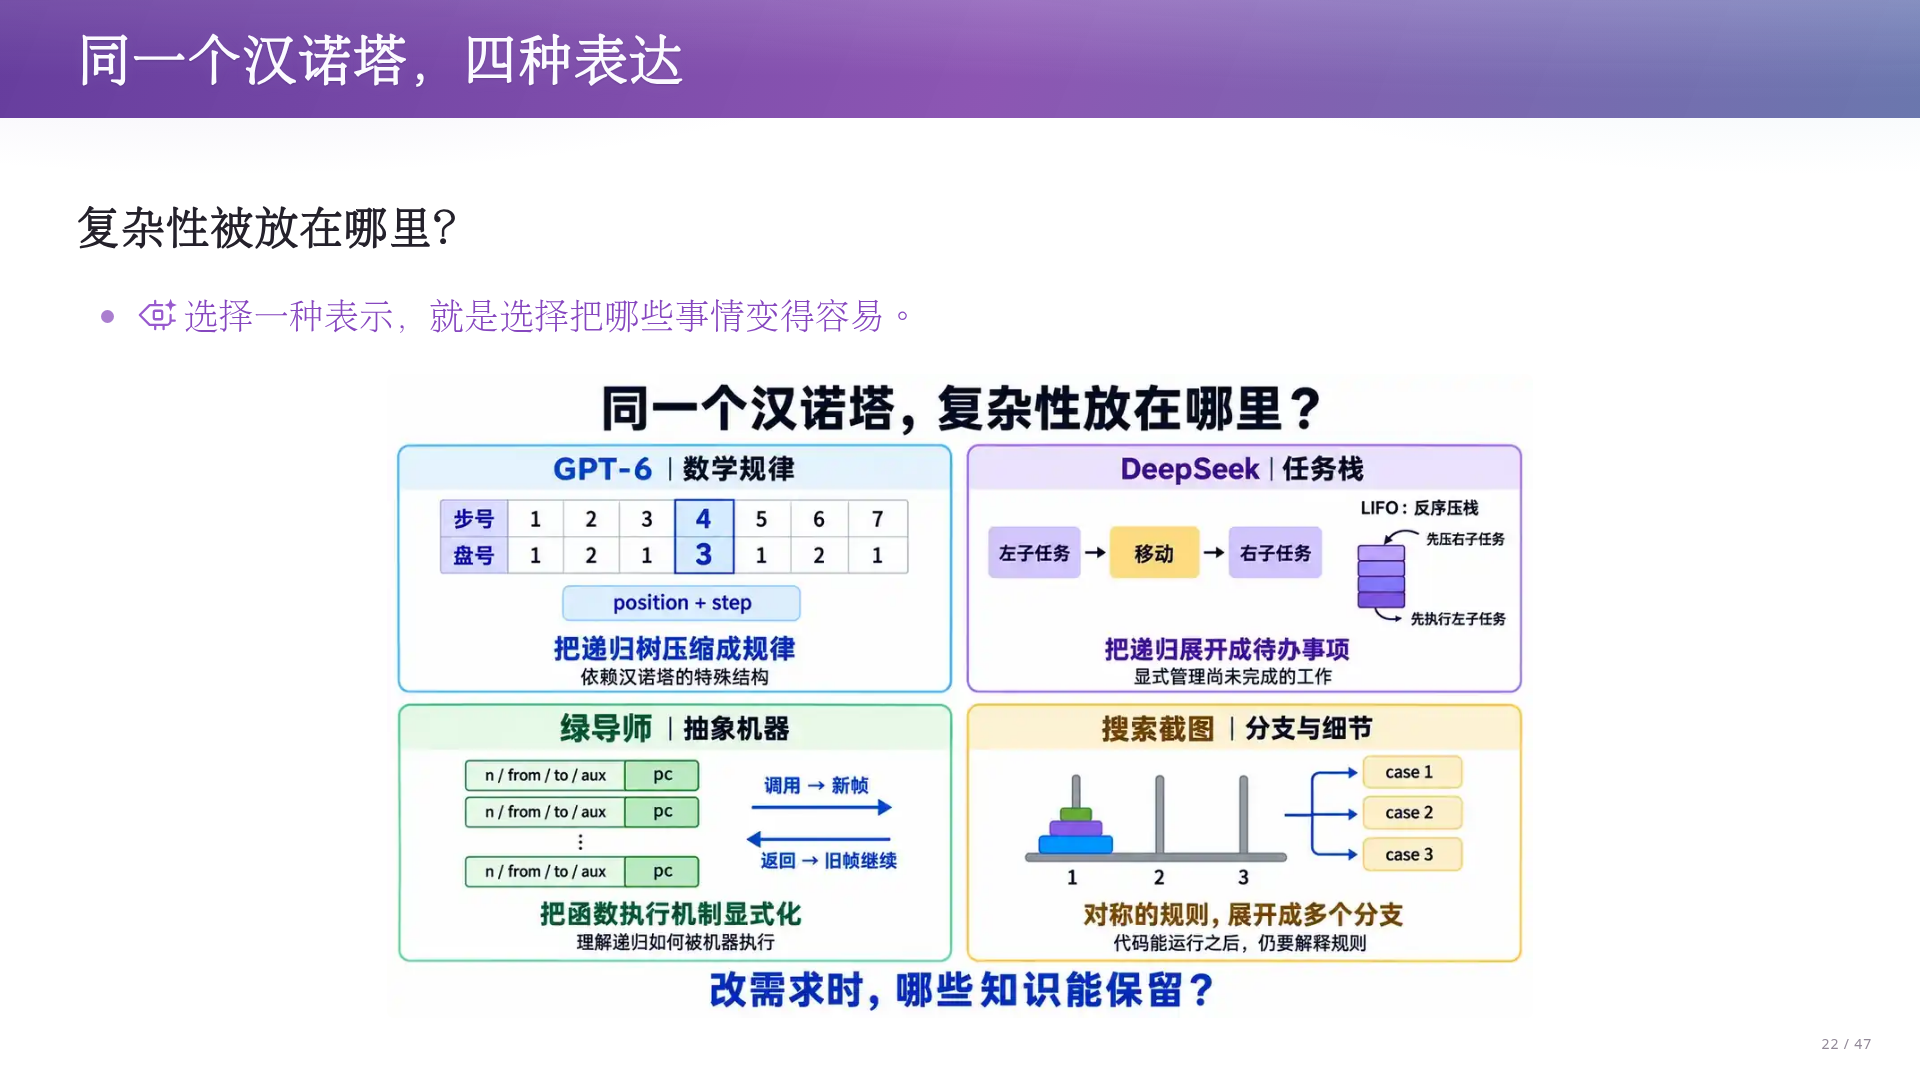
\includegraphics[width=\linewidth]{slides-images/slide-022.png}

\caption{四种表达的对照：选择表示就是选择安放复杂性（官方课件第 22 页）}

\end{figure}

将非递归汉诺塔的四种代码表达放在一起复盘：第一种表达把复杂性放在了“数学规律”里，依靠数论性质消除了递归状态，但代码与特定规则强绑定；第二种表达把复杂性放在了“任务分解（任务栈）”里，忠实反映了递归问题的领域结构，直观且易于理解；第三种表达把复杂性放在了“执行机器（抽象机器）”里，通过模拟调用栈帧与程序计数器，提供了一套可推广到任意递归过程的形式语义框架；而第四种劣质表达则没有做任何有效抽象，任由复杂性散落在混乱的“分支细节”与命名冲突中。选择一种问题表示，本质上就是选择把复杂性安放在哪里，以及选择把哪些事情变得容易处理。

从十行汉诺塔的对比中我们可以看到，“跳出问题看问题”是架构设计的核心能力：GPT 跳到数学层面看问题，DeepSeek 站在数据结构层面看问题，而系统架构师还可以站在编程语言执行语义的层面看问题。建立起这种跳出局部代码寻找合适表示的直觉后，下一章我们将把代码规模扩大到两千行，看看面对脆弱的 Excel 二维码生成需求时，如何通过构造“中间语言编译器”来化解危机。

\begin{importantbox}{Parnas 信息隐藏准则与模块边界的真伪}

把代码按顺序切分成 read\_input、parse\_input、process\_input、write\_output 四个函数，并不等于自动拥有了良好的软件架构。真正的架构边界取决于数据如何流动、谁拥有状态以及谁可以依赖谁。只有遵循 Parnas（1972）提出的信息隐藏准则，将容易变化的设计决策（如命令行参数格式或底层存储结构）严格封装在模块内部，禁止跨阶段随意修改共享全局变量，才能让一次需求变更真正被拦截在单一模块边界之内。

\end{importantbox}

\begin{knowledgebox}{跳出代码看问题：从语法细节到操作语义}

课堂强烈反对死抠语法边角料的“语言律师”式学习，主张从第一性原理（First Principles）理解编程语言构件的架构价值。例如在非递归汉诺塔中，第三种解法之所以能用十行代码优雅地消除递归，是因为直接运用了 C 语言的小步操作语义（Operational Semantics）：将整个程序的运行看作状态机，用 Frame 结构体显式接管原本隐含在底层硬件与编译器中的栈帧数据与程序计数器 pc。理解了这一层抽象，任何递归乃至互递归函数都能按统一规律转化为状态机。

\end{knowledgebox}

\begin{warningbox}{汉诺塔数学规律解法的边界条件与工程局限}

在编写或使用第一种基于二进制位运算的汉诺塔解法时，必须严格遵守两个技术约束：第一，为防止 64 位无符号整数左移发生溢出或触发 C 语言未定义行为，盘子数量必须满足 1 <= n < 64，并使用 uint64\_t total = (UINT64\_C(1) << n) - 1 计算总步数；第二，数学规律仅仅压缩了源代码行数并省去了栈空间，绝对没有消除指数级的计算复杂度，总移动步数依然是 2\textasciicircum{}n - 1 步，且一旦移动规则微调，整套数学公式便可能彻底失效。

\end{warningbox}

\par\needspace{5\baselineskip}\textbf{术语消化：十行代码与小程序中的核心架构概念对照}

\begin{center}\small\begin{tabularx}{\linewidth}{YYY}

\toprule

术语 & 解决的问题 & 机制与课程关系\\\midrule

信息隐藏 (Information Hiding) & 防止局部设计决策的变更沿着依赖关系传染给整个系统 & 将易变的实现细节（如输入格式解析、状态存储）封装在模块内部，仅通过明确契约交换数据，是划分架构边界的根本准则\\[3pt]

问题表示 (Problem Representation) & 同一逻辑问题在直接硬写时分支混乱、认知负担过高 & 通过改变编码问题的方式（如转为二进制规律、显式任务栈或抽象机器），重新分配复杂性的归处，降低实现与维护难度\\[3pt]

显式任务栈 (Explicit Task Stack) & 在不使用语言原生递归调用的前提下保存尚未完成的子任务 & 将待处理的盘数与柱子角色封装为 Task 结构体，按执行顺序的反方向压入 LIFO 栈中循环消费，直接对应递归的任务分解树\\[3pt]

抽象机器与小步语义 (Abstract Machine \& Operational Semantics) & 提供一套不依赖特定题目规律、能将任意递归过程转化为非递归循环的通用机制 & 显式构造包含局部变量与程序计数器 pc 的栈帧 Frame，用 call/ret 宏和 switch(f->pc) 模拟函数调用的单步状态转移\\[3pt]

\bottomrule\end{tabularx}\end{center}

\begin{lstlisting}[basicstyle={\ttfamily\small\linespread{1}\selectfont},captionpos=t,caption={十行非递归汉诺塔的三种核心表示：数学规律、任务栈与抽象机器}]
// 1. 数学规律表示 (限定 1 <= n < 64, uint64_t total = (UINT64_C(1) << n) - 1)
for (uint64_t step = 1; step <= total; step++) {
    int disk = 1;
    for (uint64_t x = step; (x & 1) == 0; x >>= 1) disk++;
    int direction = (n - disk) % 2 == 0 ? -1 : 1;
    int from = position[disk], to = (from + direction + 3) % 3;
    printf("Move disk %d: %c -> %c\n", disk, pegs[from], pegs[to]);
    position[disk] = to;
}

// 2. 显式任务栈表示 (限定 n >= 1，LIFO 逆序压栈分解子任务)
assert(n >= 1);
push(&s, n, A, B, C);
while (!isEmpty(&s)) {
    Task t = pop(&s);
    if (t.n == 1) printf("%c -> %c\n", t.src, t.dst);
    else {
        push(&s, t.n - 1, t.aux, t.src, t.dst);
        push(&s, 1, t.src, t.aux, t.dst);
        push(&s, t.n - 1, t.src, t.dst, t.aux);
    }
}

// 3. 抽象机器表示 (限定 1 <= n < 64；用整数栈深 sp 避免数组首元素之前的越界指针)
Frame stk[64];
int sp = 0;
#define call(...) (assert(sp < 64), stk[sp++] = (Frame){.pc = 0, __VA_ARGS__})
#define ret() (assert(sp > 0), --sp)
assert(n >= 1);
call(n, from, to, aux);
while (sp > 0) {
    Frame *f = &stk[sp - 1];
    int next_pc = f->pc + 1, cur_n = f->n;
    char f_from = f->from, f_to = f->to, f_aux = f->aux;
    f->pc = next_pc;
    switch (next_pc - 1) {
        case 0: if (cur_n == 1) { printf("%c -> %c\n", f_from, f_to); ret(); } break;
        case 1: call(cur_n - 1, f_from, f_aux, f_to); break;
        case 2: call(1, f_from, f_to, f_aux); break;
        case 3: call(cur_n - 1, f_aux, f_to, f_from); break;
        case 4: ret(); break;
        default: assert(0);
    }
}
\end{lstlisting}

输入为盘子总数 n 及三根柱子的标识，输出为将所有盘子从起始柱搬运到目标柱的合法移动序列。三段代码完成完全相同的外部功能，但展现了三种截然不同的架构表示：第一段利用步号二进制末尾零的个数与奇偶方向直接计算状态（需满足 1 <= n < 64，总步数仍为 2\textasciicircum{}n - 1）；第二段在 \texttt{n >= 1} 的前提下用显式栈逆序保存待执行的分解任务；第三段通过维护栈帧数组 \texttt{stk}、整数栈深 \texttt{sp} 与程序计数器 \texttt{pc} 模拟 C 语言函数调用的小步操作语义，相比课件原图的指针示意进一步补齐了标准 C 边界与容量检查。

\needspace{7\baselineskip}\subsection{本章小结}

本章阐明了软件架构的核心职责：\textbf{安放复杂性并隔离变化}。架构设计并非大型分布式系统的专利，从小程序的四阶段划分、getopt 参数解析，到十行非递归汉诺塔的编写，处处都体现着 Parnas 的信息隐藏准则与语言语义约束。

通过对比汉诺塔的数学规律、任务栈、抽象机器与劣质分支代码四种表达，我们看到：\textbf{选择一种问题的表示方式}，就是选择把复杂性放在哪里，以及让哪些未来的变化更容易应对。

\needspace{8\baselineskip}\section{第四章 两千行代码的架构：把 Excel 二维码生成器看作编译器}

上一章通过十行汉诺塔代码证明了：选择不同的表示方式，就是选择将复杂性安放在哪里。当程序规模从十行扩大到两千行，面对在 Excel 工作表中动态生成二维码的需求时，直接让 Agent 硬写单元格公式会迅速陷入括号配对与引用耦合的泥潭。本章将探讨如何运用“跳出问题看问题”的思维，识别出算法描述与目标运行环境之间的鸿沟，通过引入中间语言（IR）和双后端编译器架构，把输入绑定、布局分配、版本兼容、语义验证与性能优化解耦到各自的模块边界中。

\subsection{跳出问题看问题的能力来源}

在非递归汉诺塔的例子中，无论是运用位运算规律、任务栈还是抽象状态机，核心都在于跳出“眼前该写哪个分支”的局限，站在更高的抽象层次重新审视问题。当系统规模上升到两千行时，工程师需要思考：这种跨层次选择恰当表示的架构能力，究竟是从哪里习得的？

\begin{figure}[H]\centering


\includegraphics[width=\linewidth]{slides-images/slide-023.png}

\caption{跳出问题看问题的能力来源（官方课件第 23 页）}

\end{figure}

课件指出，\textbf{跳出问题看问题}的视野建立在多层次的规律之上：代码之外有客户工作的业务规律，客户之外有社会运行的规律，社会之外还有数学与物理世界的规律。

这种架构直觉并非凭空产生，而是源于学校里的系统学习与社会中积累的真实经验。

课堂上讲师也提出了一个开放性思考：我们对好设计的学习本质上是将经验压缩为理解，再\textbf{从第一性原理}（First Principles）出发推导方案；至于这种跨层次抽象能力未来能否通过强化学习完全习得，仍需持续观察，不能把今天的能力边界当成永久边界。

理解代码之外的规律，要求开发者走出纯技术视角。例如课堂提到的教务系统场景，理解一位临近退休的教务老师“希望字大一点、别误点旁边按钮”的操作习惯，需要社会经验与共情；而理解如何把复杂计算塞进电子表格，则需要编译原理的学科训练。接下来我们就看一个具体的两千行级任务：Excel 二维码生成器。

\subsection{直接生成 Excel 公式的脆弱性与变更困境}

来看一个明确的需求：在 Excel 工作表的某个单元格中输入字符串，完全依靠工作表公式实时计算并在单元格网格中显示对应的二维码；当用户修改输入文本时，二维码图案随之自动重算更新。如果直接让 AI Agent 为每个单元格生成公式，会遭遇怎样的工程困境？

\begin{figure}[H]\centering

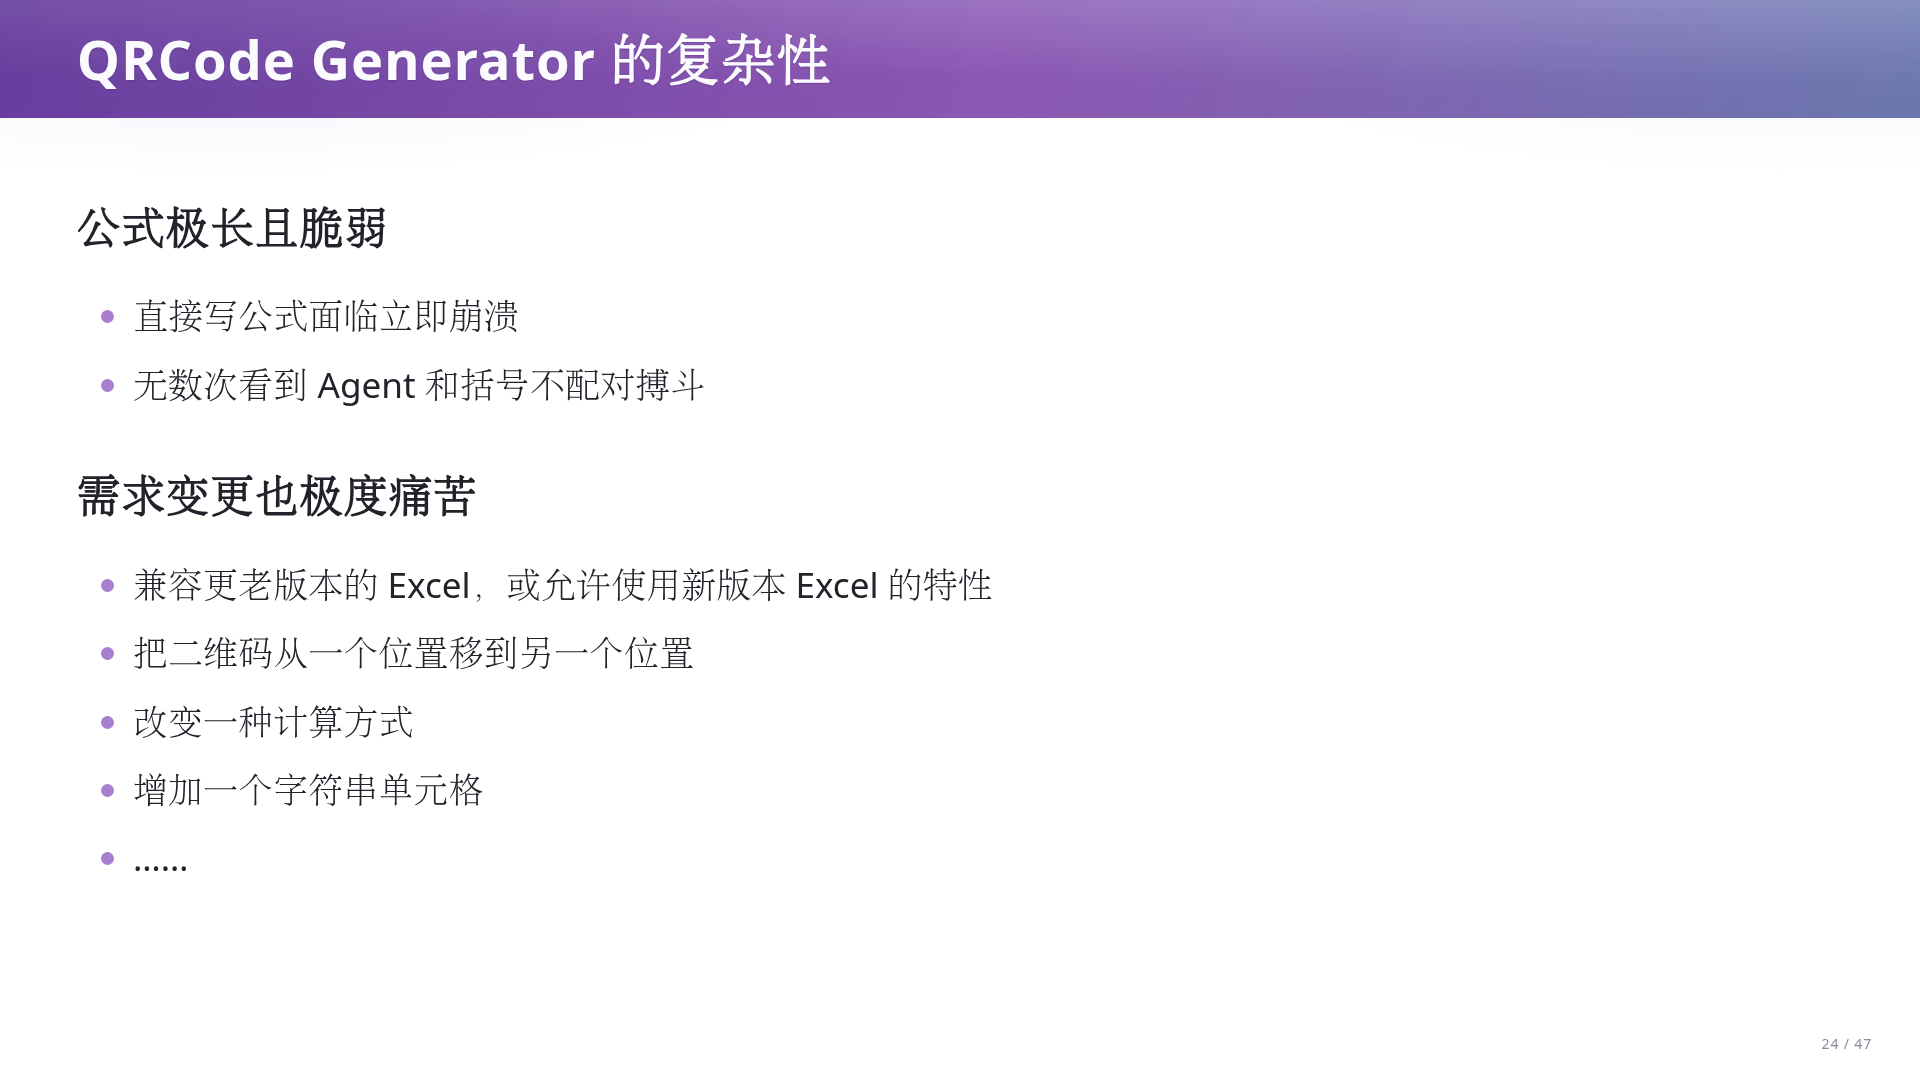
\includegraphics[width=\linewidth]{slides-images/slide-024.png}

\caption{直接生成 Excel 公式的脆弱性与变更困境（官方课件第 24 页）}

\end{figure}

直接编写公式会立刻撞上两座大山。第一是公式极长且脆弱：二维码生成涉及字节编码、多项式长除、伽罗瓦域查表与掩码异或，把这些步骤直接塞进公式，会导致括号、单元格引用与数组运算死死缠绕，Agent 往往要耗费大量时间与成百上千个不配对的括号搏斗。第二是需求变更极度痛苦：一旦要求兼容没有新函数的老版本 Excel、把二维码图案在表内整体平移一格、更换某种计算方式，或者增加一个字符串输入单元格，原本看似局部的改动都会穿透整片硬编码公式，导致推倒重来。

课堂提示指出，Excel 本质上是为财务报表与轻量级数据管理设计的，并非围绕通用图灵完备计算构建的编程环境。比如查找功能从早期的 VLOOKUP 演进到较新的 XLOOKUP，如果 AI 直接按最新语法把公式写死，一旦交付给使用旧版软件的办公电脑就会全部失效。要摆脱这种脆弱性，必须跳出 Excel 公式本身。

\subsection{把二维码生成器重新定义为小型编译器}

既然直接写公式维护成本极高，我们不妨跳出表格看问题：二维码生成算法本身有清晰的国际标准，用 Python 或伪代码实现只需几百行，真正的困难在于如何把通用的算法步骤映射到受限的电子表格环境中。这实际上是一个典型的编译问题。

\begin{figure}[H]\centering


\includegraphics[width=\linewidth]{slides-images/slide-025.png}

\caption{把二维码生成器重新定义为小型编译器（官方课件第 25 页）}

\end{figure}

解决思路是在高级算法与目标表格之间引入一层中间表示，即 IR（Intermediate Representation，中间语言）：一种显式记录计算节点及其数据依赖关系的结构化计算图。在这套老师设想的架构中，开发者使用 Python 的函数和循环来构造计算图，并严格区分“生成时”与“运行时”：生成时按照选定的二维码容量，将 Python 循环展开为有限步的计算节点；运行时则将用户的字符串输入保留为符号节点，且凡是由输入内容决定的条件分支，都必须构造成图中的 Select(cond, a, b) 条件选择节点，留给 Excel 在用户修改单元格后动态重算判断。

讲义特别提醒：严禁在 Python 构造阶段把用户输入的字符串当作已知常量直接求值。如果分支判断在 Python 运行期就被算完了，生成器最终吐出的只是一张写死 0 和 1 的静态二维码快照，完全丧失了“修改单元格文本后自动更新二维码”的动态工作表能力。

\subsection{一份中间语言驱动双后端执行}

当算法逻辑被抽象成由基本算子构成的中间语言（IR）计算图后，计算规则的“表达”与最终在哪个平台上“执行”就分离开来。利用同一份计算图派生出两条不同的后端流水线，可以同时解决调试困难与交付生成的难题。

\begin{figure}[H]\centering

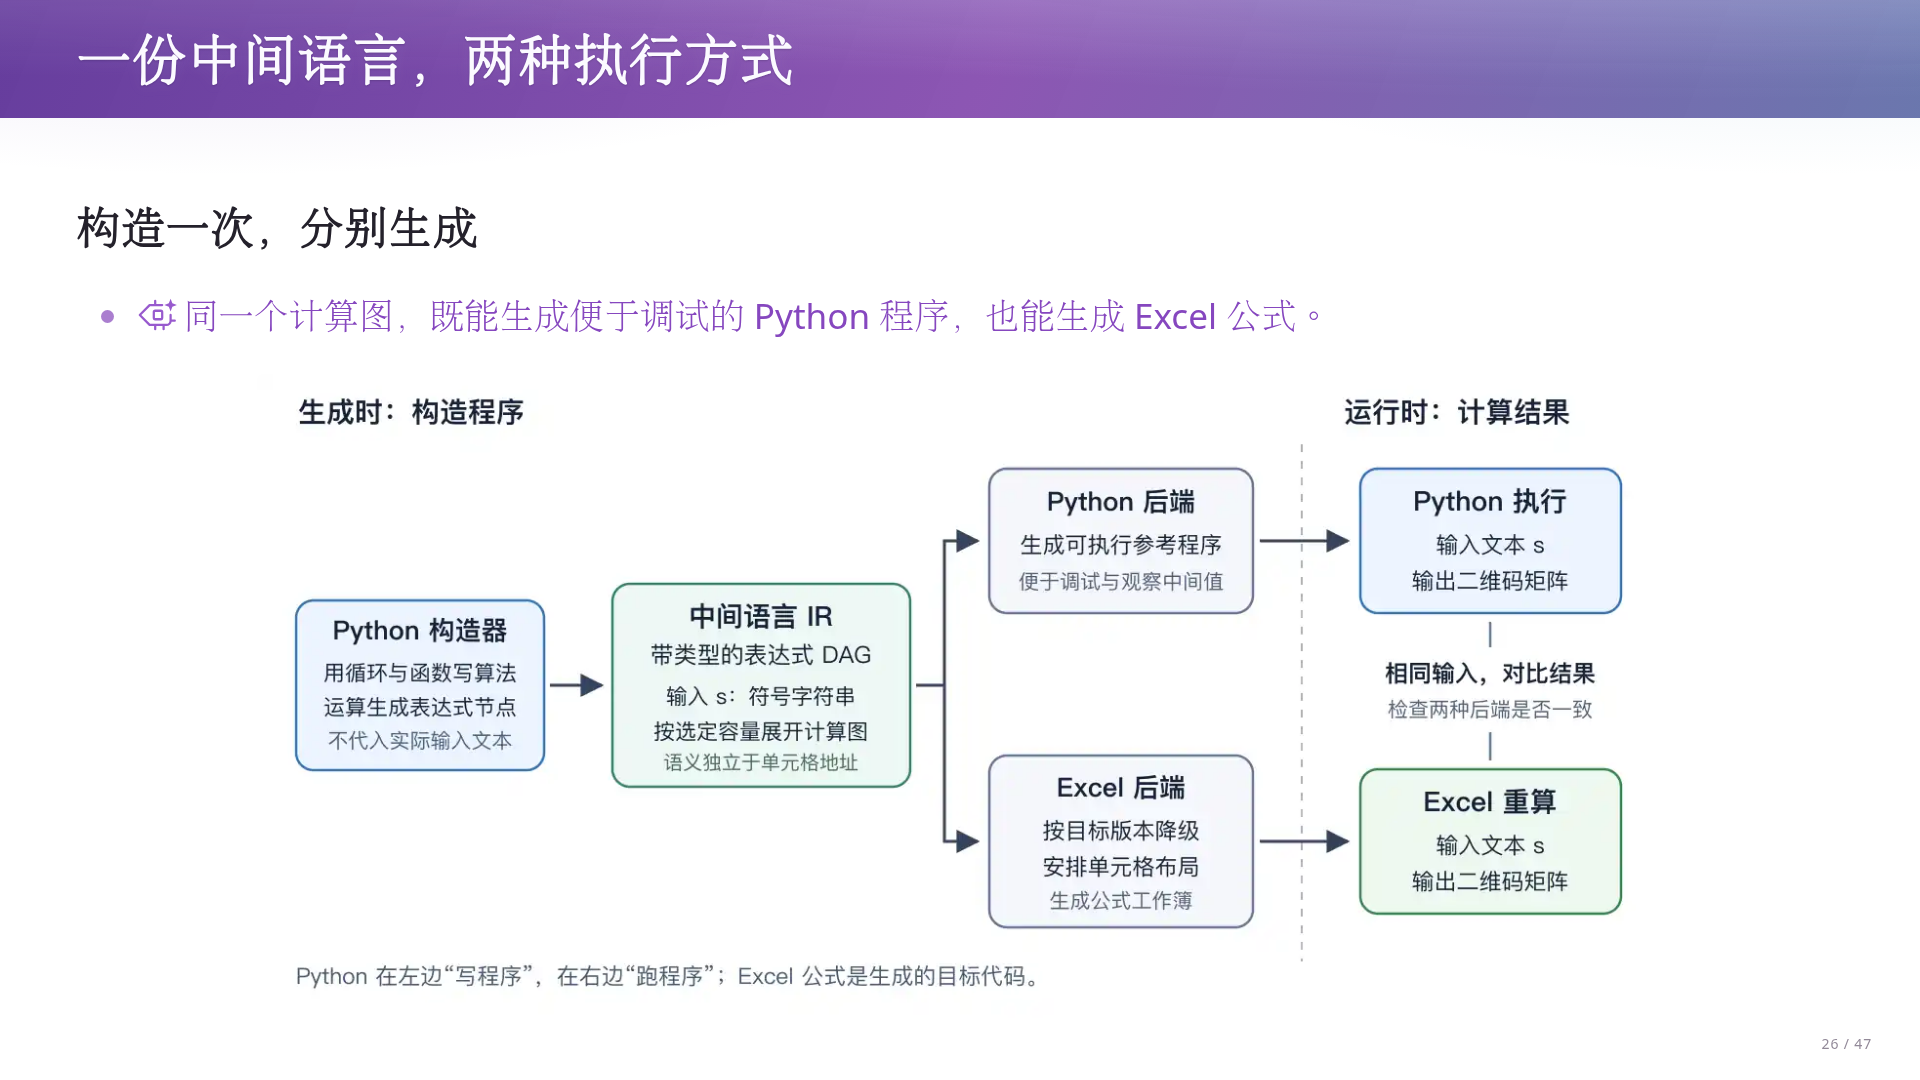
\includegraphics[width=\linewidth]{slides-images/slide-026.png}

\caption{一份中间语言驱动双后端执行（官方课件第 26 页）}

\end{figure}

如课件架构图所示，顶层的 Python 构图程序只运行一次，产出一份统一的中间语言（IR）计算图。随后，两条独立的后端分别消费这张图：左侧后端将其翻译为结构清晰、便于单步调试和快速求值的 Python 程序；右侧后端则按照电子表格的语法规则，将图中的节点与依赖关系翻译为目标 Excel 公式与工作表布局。这就像编译器前端生成统一的抽象语法树或中间码，再由不同后端生成不同架构的机器码。

这种“构造一次，分别生成”的设计，与命令行程序用 getopt 先将参数解析为中间状态再执行后续逻辑异曲同工。在直接写 Excel 公式时，某一步多项式纠错算错了几乎无法肉眼排查；而有了 Python 后端，开发者可以先在熟悉的编程环境里验证整张计算图的逻辑，再放心地交给公式后端去处理括号拼接与地址映射。

\subsection{运用信息隐藏让需求变更各就各位}

前面提到，直接生成公式时，任何微小的需求调整都会引发全局雪崩。引入中间表示和编译器分层之后，我们需要检验这套架构是否真正做到了“变化有边界”：当那四类令人头疼的需求变更再次来袭时，修改动作会被限制在哪些模块内部？

\begin{figure}[H]\centering


\includegraphics[width=\linewidth]{slides-images/slide-027.png}

\caption{运用信息隐藏让需求变更各就各位（官方课件第 27 页）}

\end{figure}

通过围绕可能变化的决策划分模块，核心算法只认识抽象符号 Input("text")，而输入绑定与布局模块才知晓它对应工作表中的 Input!B2。如表所示：第一，兼容不同版本 Excel 时，只需修改“目标能力”模块，由其选择可用函数或等价的降级实现；第二，平移二维码位置时，只需调整“布局”模块统一重新分配单元格地址并解析符号引用；第三，改变计算方式时，只需在“算法构造或优化规则”中替换对应子图并保持接口语义不变；第四，增加字符串单元格时，则在“输入绑定与组合规则”中登记新输入，明确拼接、编码与容量计算方式。

这一设计直接呼应了 David Parnas 在 1972 年提出的模块分解准则：模块划分不应只按执行流程图切分，而应围绕困难的、可能变化的设计决策来进行，并将这些易变决策隐藏在稳定的接口后面。当算法、输入绑定、地址布局和目标函数库各司其职，需求变更就有了明确的归处。

\subsection{中间语言的明确语义与多维交叉验证}

把系统拆成中间语言和两个后端，并不意味着把代码切成几个文件就万事大吉。如果中间语言本身的运算语义含糊不清，Python 后端和 Excel 后端各自按默认习惯去猜测，两边算出来的结果就会南辕北辙。此外，如何严格验证生成的二维码是正确的？

\begin{figure}[H]\centering

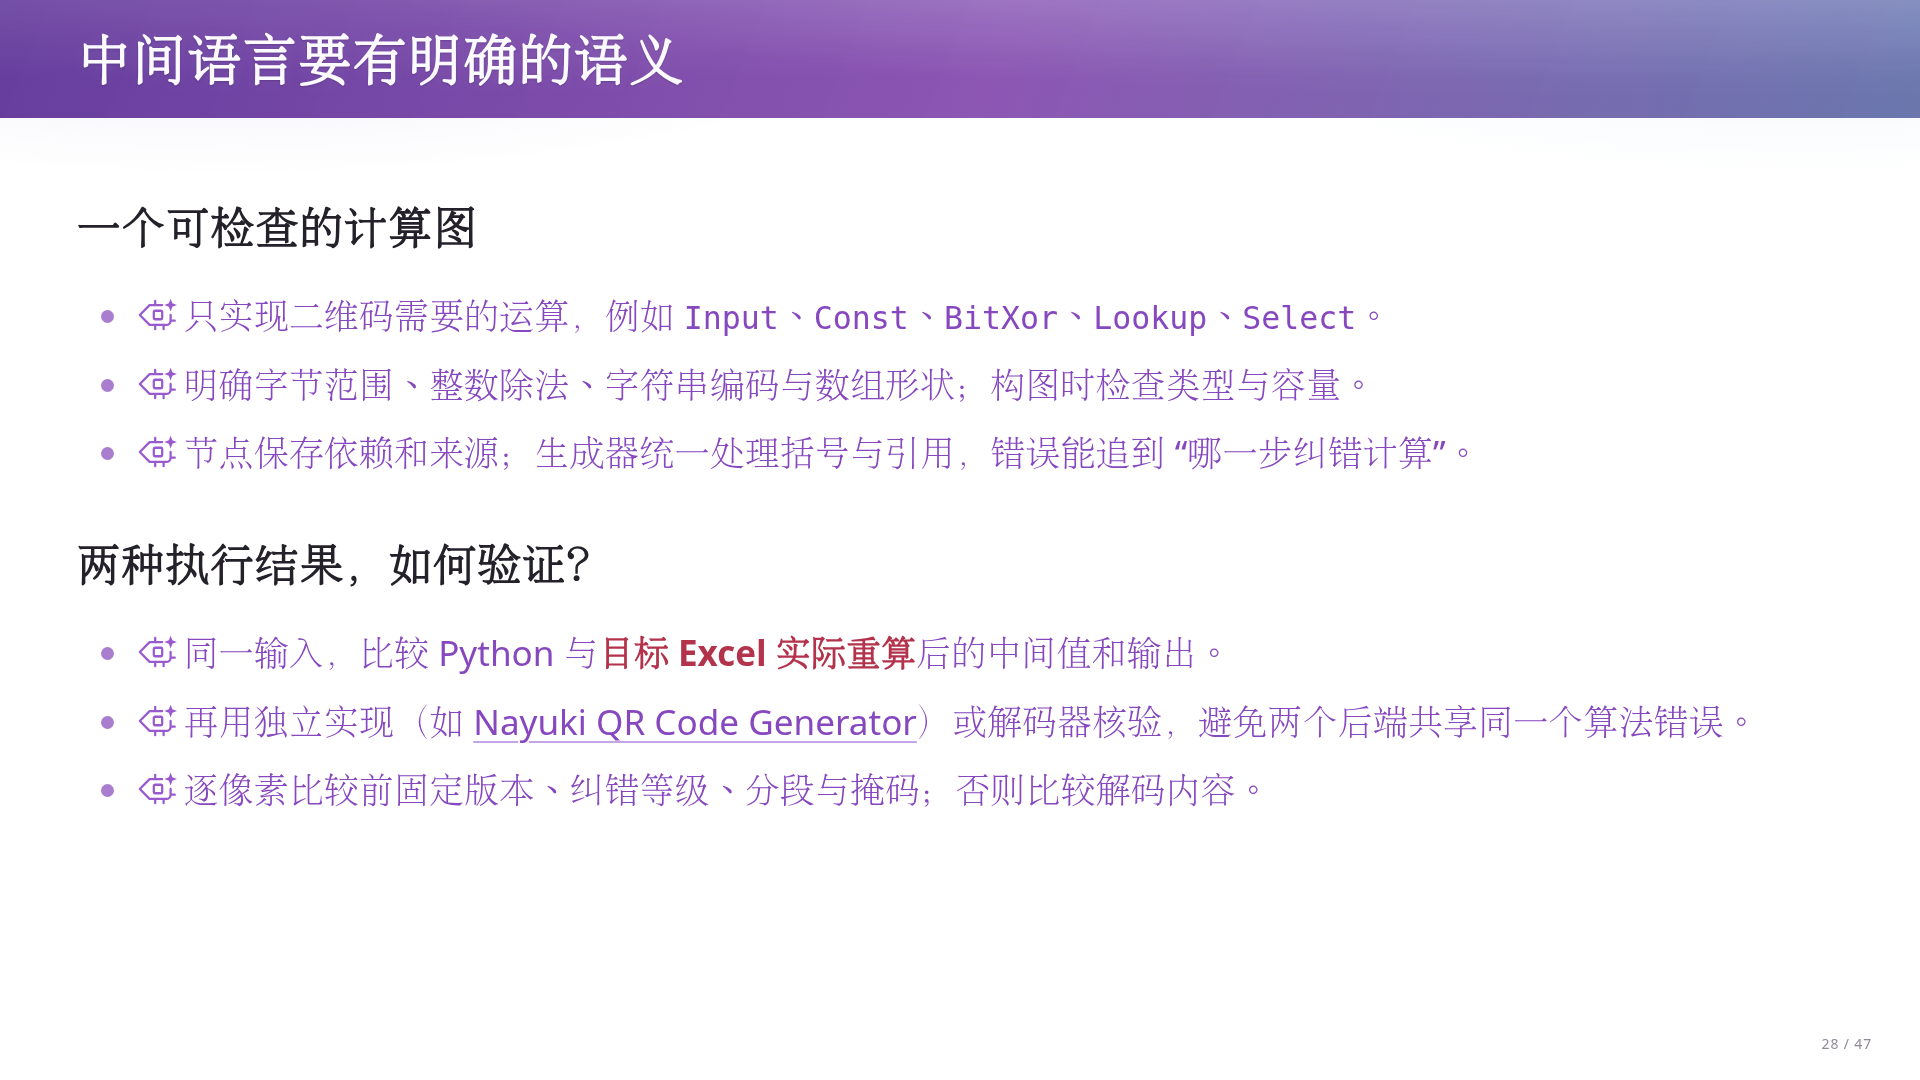
\includegraphics[width=\linewidth]{slides-images/slide-028.png}

\caption{中间语言的明确语义与多维交叉验证（官方课件第 28 页）}

\end{figure}

中间语言必须拥有自己严格的形式语义。计算图只纳入二维码必需的算子，如 Input、Const、BitXor、Lookup、Select；同时必须明确定义字节取值范围、整数除法截断方式、字符串编码与数组形状，并在构图阶段静态检查类型与容量限制。每个节点还保存数据依赖与源码来源，由公式生成器统一处理括号与引用，使报错能精准追溯到具体哪一步纠错计算。在验证方面，首先对同一输入比较 Python 后端与目标 Excel 实际重算后的中间值及输出；其次必须引入独立实现（如 Nayuki QR Code Generator）或独立二维码解码器进行交叉核验。

这里有两条关键的技术核查准则：第一，Python 后端与 Excel 后端结果一致，绝不等于二维码算法完全正确，因为二者共用同一份 IR 计算图，完全可能共享同一个算法逻辑错误；第二，若要与外部参考库逐像素比对矩阵，必须事先固定二维码版本、纠错等级、编码分段策略与掩码编号（0 到 7），因为不同合规参数生成的图案外观不同但都能被正确扫码还原。

\subsection{基于计算图改写与实际重算成本的性能优化}

即使生成的 Excel 公式在逻辑上完全正确，如果把所有计算都无脑展开成巨型公式，工作表不仅体积庞大，每次修改输入后的重算延迟也会极其严重。在编译器架构下，性能优化不再是手改零散公式，而是成为计算图改写与后端代码生成策略的系统工程。

\begin{figure}[H]\centering


\includegraphics[width=\linewidth]{slides-images/slide-029.png}

\caption{基于计算图改写与实际重算成本的性能优化（官方课件第 29 页）}

\end{figure}

优化分为两个层次。首先在计算图层面做等价改写：一是“常量折叠”，将固定参数下的定位图案、有限域对数与反对数常量表在生成时直接算好；二是“公共子表达式消除”，将图中相同的纯计算合并共享为同一个节点，避免把同一段长公式到处复制粘贴。其次在后端落表层面权衡：单个公式内部复用变量可使用 Excel 的 LET 函数；跨公式共享或目标版本不支持 LET 时，则将中间结果拆分到辅助单元格中。最终应依据 Excel 实际计算成本做选择，结合节点复用次数、计算量与目标版本公式长度限制，决定内联还是拆格，并分别测量首次完整计算时间、修改输入后的重算时间及工作簿文件体积。

Microsoft 官方的 Excel 性能指南同样建议拆解巨型公式、减少重复计算并利用辅助单元格缓存中间结果。通过引入 IR，这些领域优化规则与编译器的 Profile-Guided Optimization（基于性能剖析的优化）自然结合，既防止了公式膨胀，又避免了盲目缓存导致工作簿体积失控。至此，两千行代码的编译器架构完整闭环，下一章我们将迈向五十万行的教务系统。

\begin{importantbox}{区分编译器的生成时（Build-time）与运行时（Run-time）}

在用 Python 构造 Excel 二维码计算图时，必须严格划清两个阶段的边界：二维码的版本容量、定位图案坐标、伽罗瓦域查表常量以及固定次数的循环展开，属于生成时（Python 运行期）确定的结构；而用户在单元格中填写的具体字符串，必须表示为 Input("text") 符号节点，所有依赖输入内容的条件分支必须表示为 Select(cond, a, b) 节点，留到运行时由 Excel 动态重算求值。

\end{importantbox}

\begin{knowledgebox}{课堂直觉：用通用编译思维降维打击受限环境}

为什么用 Python 写二维码生成只需几百行，直接在工作表里维护整套二维码公式却如此痛苦？尽管现代 Excel 已引入 \texttt{LET}、\texttt{LAMBDA}、\texttt{REDUCE} 等函数，但若要兼容不支持这些特性的旧版本或受限于基础公式子集，就难以直接表达循环与局部作用域；即便在现代版本中，跨单元格的数据依赖、公式长度限制与版本能力差异依然会让手写公式产生高昂的生成与维护成本。跳出“硬写公式”的定式，把 Python 当作元语言（Meta-language）去生成中间表示，再由后端自动管理括号配对、单元格地址映射和版本适配，就能把繁琐的公式拼接转化为清晰的编译流水线。

\end{knowledgebox}

\begin{warningbox}{验证陷阱：双后端一致不等于算法无误，逐格对比需固定参数}

切忌认为“Python 后端输出与 Excel 重算结果完全一致”就证明二维码生成器没有 Bug。由于两个后端翻译自同一张 IR 计算图，若构图阶段把多项式生成元或掩码规则写错，两边会忠实地算出完全相同的错误图案。必须引入独立解码器验证扫码还原文本；若与 Nayuki 等独立库做逐像素对比，则必须先固定版本号、纠错等级、分段模式与掩码（0-7），否则合规的不同选择也会产出不同矩阵。

\end{warningbox}

\par\needspace{5\baselineskip}\textbf{术语消化：Excel 二维码编译器架构的核心概念与职责映射}

\begin{center}\small\begin{tabularx}{\linewidth}{YYY}

\toprule

架构概念 / 术语 & 解决的核心问题 & 运行机制与课程关系\\\midrule

中间语言（IR） & 解耦二维码算法描述与目标平台（Excel/Python）的具体语法 & 以包含 Input、Const、BitXor、Lookup、Select 的有向无环计算图显式记录运算与数据依赖\\[3pt]

符号输入与 Select 节点 & 防止在生成阶段把用户输入硬编码算死，保留工作表动态重算能力 & 将输入单元格抽象为符号，受输入影响的分支转为图节点，交由 Excel 运行时求值\\[3pt]

信息隐藏（Parnas 准则） & 隔离版本兼容、图案平移、新增输入等频繁变化的设计决策 & 将目标函数选择、单元格地址分配、输入拼接规则分别封装在独立模块接口之后\\[3pt]

常量折叠与公共子表达式共享 & 消除重复计算与巨型长公式，降低工作簿体积与重算延迟 & 生成时预计算固定图案与有限域表；图中合并相同纯计算，落地时结合 LET 或辅助单元格拆格\\[3pt]

\bottomrule\end{tabularx}\end{center}

\begin{lstlisting}[basicstyle={\ttfamily\small\linespread{1}\selectfont},captionpos=t,caption={构造中间表示（IR）并分别生成 Python 与 Excel 公式的核心机制示意}]
class Node:
    pass

class Input(Node):
    def __init__(self, name: str): self.name = name

class Const(Node):
    def __init__(self, val: int): self.val = val

class BitXor(Node):
    def __init__(self, a: Node, b: Node): self.a, self.b = a, b

class Select(Node):
    def __init__(self, cond: Node, t: Node, f: Node):
        self.cond, self.t, self.f = cond, t, f

def emit_python(node: Node) -> str:
    if isinstance(node, Input): return f"inputs['{node.name}']"
    if isinstance(node, Const): return str(node.val)
    if isinstance(node, BitXor): return f"({emit_python(node.a)} ^ {emit_python(node.b)})"
    if isinstance(node, Select):
        return f"({emit_python(node.t)} if {emit_python(node.cond)} else {emit_python(node.f)})"
    raise TypeError(f"Unsupported IR node: {type(node).__name__}")

def emit_excel(node: Node, layout: dict) -> str:
    if isinstance(node, Input): return layout[node.name]
    if isinstance(node, Const): return str(node.val)
    if isinstance(node, BitXor):
        a, b = emit_excel(node.a, layout), emit_excel(node.b, layout)
        return f"BITXOR({a},{b})"
    if isinstance(node, Select):
        c = emit_excel(node.cond, layout)
        t = emit_excel(node.t, layout)
        f = emit_excel(node.f, layout)
        return f"IF({c},{t},{f})"
    raise TypeError(f"Unsupported IR node: {type(node).__name__}")
\end{lstlisting}

输入为抽象节点构成的 IR 计算图与单元格布局字典 \texttt{layout}（如 \texttt{\{'text': 'Input!B2'\}}），输出分别为可执行的 Python 表达式字符串与支持 \texttt{BITXOR} 的现代 Excel 公式字符串（对未知节点显式抛出 \texttt{TypeError}）。代码展示了算法构图阶段如何使用符号节点 \texttt{Input} 和条件节点 \texttt{Select}，并由两个后端各自处理括号与目标语法，实现“构造一次、双端生成”。

\needspace{7\baselineskip}\subsection{本章小结}

本章以两千行规模的 Excel 二维码生成器为例，展示了如何通过“跳出问题看问题”将复杂的电子表格公式生成任务转化为\textbf{小型编译器架构}。

通过定义语义明确的\textbf{中间表示（IR）}，严格区分生成时循环展开与运行时符号求值，并依据 Parnas 信息隐藏准则拆分输入绑定、地址布局、目标版本适配与图优化模块，使系统能够从容应对需求变更、完成双后端加独立解码器的严密验证。

\needspace{8\baselineskip}\section{第五章 五十万行系统的困境：CRUD 的有损投影与语义漂移}

从十行汉诺塔的表示选择，到两千行二维码生成器的中间语言解耦，我们已经看到架构如何安放复杂性并隔离变化。当系统规模膨胀到五十万行级别的高校教务系统时，架构的核心矛盾依然是“怎样看待问题”。如果沿用最直观的“只覆写当前状态快照”的 CRUD（创建、读取、更新、删除）建模思路，不保存历史过程与决策依据，为什么会在长期的政策调整、线下特批与组织机构变迁中，一步步陷入数据黑洞与语义改写的困境？本章将深入剖析当前状态背后隐藏的数据依赖与历史丢失问题。

\subsection{五十万行教务系统：从 AI 原型审视架构起点}

当代码规模从几千行跃升到五十万行，人们谈论架构时往往立刻联想到分布式数据库、微服务或流式计算框架。然而在引入重型组件之前，更根本的问题是我们选择用什么模型去映射现实业务。我们可以从现成教务系统的直观体验出发，看看当 AI 快速搭建系统原型时，它默认选择了怎样的架构视角。

\begin{figure}[H]\centering


\includegraphics[width=\linewidth]{slides-images/slide-030.png}

\caption{五十万行教务系统：从 AI 原型审视架构起点（官方课件第 30 页）}

\end{figure}

课件指出，面对五十万行规模的教务系统，架构的本质依然是“\textbf{跳出问题看问题}”。当 AI 具备强大的代码生成能力后，最直接的尝试就是先观察现有教务系统的功能表现，然后让 AI 根据整理出的需求说明书直接搓出一个最小可行产品（MVP）。这种快速落地的尝试，正好为我们提供了一个审视\textbf{默认架构选择}的真实样本。

在课堂演示中，老师让 AI 调研教务系统教师端功能并生成需求文档，随后启动子代理直接编写出一个可交互的教务系统原型。这个原型包含了教学任务查看、教材编辑、学生名单与缺课次数维护等功能。表面上看，AI 在极短时间内走通了从意图到实现的全流程，但紧接着我们就需要打开代码库，检查它内部究竟长什么样。

\subsection{AI 生成的单体原型与大文件堆积}

AI 能够写出表面功能完备、界面交互流畅的教务系统演示程序，但这种“一次成型”的代码在结构上是如何组织的？当机器不需要像人类那样受限于单文件阅读记忆容量时，它会傾向于写出怎样的模块结构？从源码结构中，我们可以直接观察文件体积以及业务逻辑在代码中的分布方式。

\begin{figure}[H]\centering

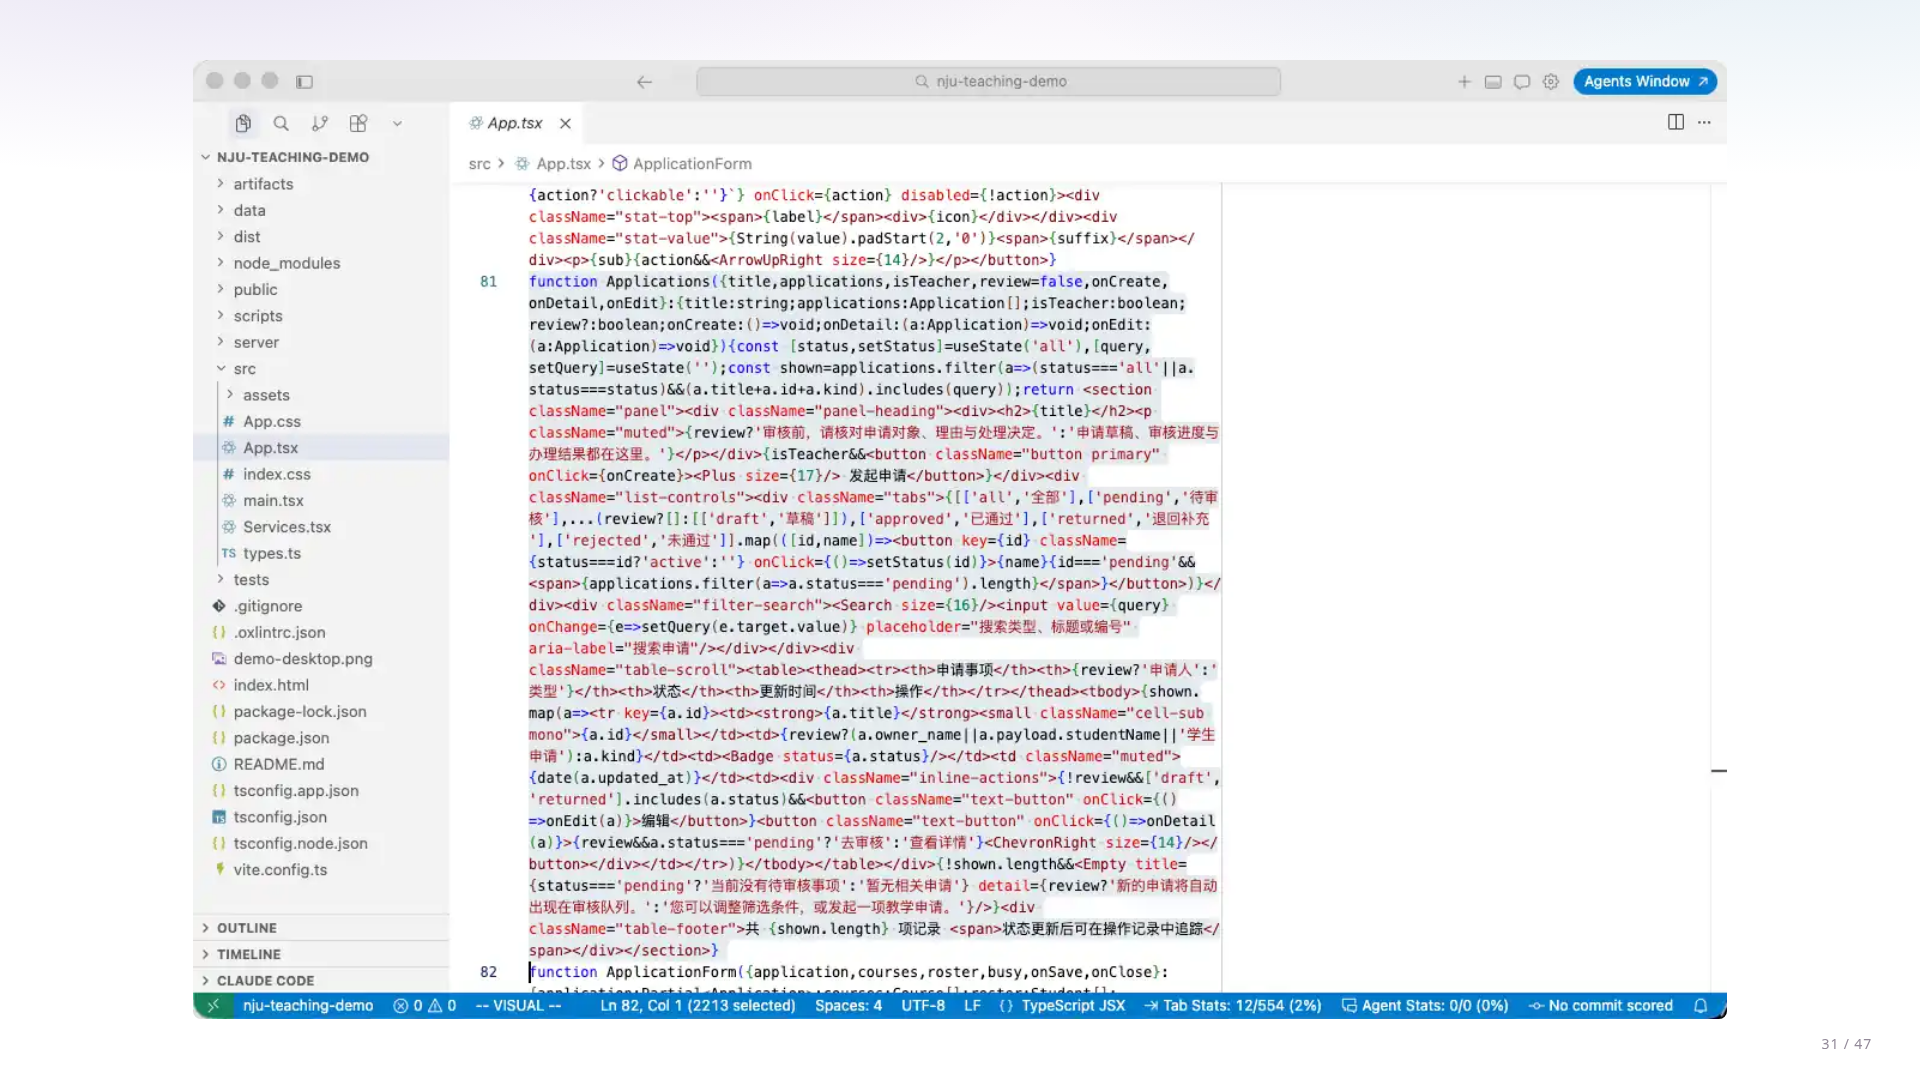
\includegraphics[width=\linewidth]{slides-images/slide-031.png}

\caption{AI 生成的单体原型与大文件堆积（官方课件第 31 页）}

\end{figure}

观察 AI 生成的教务系统演示原型的代码组织结构：在未受额外架构约束的情况下，模型生成了一个高度集中的单体系统：前端与交互逻辑被塞进一个高达 83 KB 的 TSX 文件中，而后端的业务处理逻辑则挤在一个 38 KB 的 Service 文件里，初期甚至把大量逻辑紧凑地写在同一函数体中，经格式化工具整理后才呈现出可阅读的排版。

尽管代码集中在两个巨型文件中，但课堂分析发现，AI 生成的实现并非毫无章法，它在代码里自然融入了乐观锁（提交更新时校验版本号以防并发覆盖）、幂等性（同一请求重复执行不产生额外副作用）、事务、审计日志和统一错误码等生产级横切设计。然而，局部工程技巧的熟练，并不能掩盖整体业务结构高度耦合的隐患。

\subsection{大文件单体的演化困境：新增功能如同拆盲盒}

一个拥有乐观锁、审计日志和前后端分离结构的原型，为什么仍然潜藏着巨大的维护危机？为了客观评估这份代码的演进潜力，课堂上老师开启了一个独立的对话会话，让模型以架构评审的视角审视这组巨型文件。模型对自身生成的代码给出了直接的架构诊断。

\begin{figure}[H]\centering


\includegraphics[width=\linewidth]{slides-images/slide-032.png}

\caption{大文件单体的演化困境：新增功能如同拆盲盒（官方课件第 32 页）}

\end{figure}

课件引用了模型对这份教务系统原型的架构评价：虽然当前系统采用了经典的三层单体与前后端分离结构，具备一定的可维护性，但它本质上是把所有业务逻辑硬挤在几个大文件里的演示原型。如果不及时进行模块拆分并统一业务规则表达，后续每增加一项新功能，都会因为内部状态交织而变得越来越像“拆盲盒”。

为什么在巨型文件上继续叠加功能会像拆盲盒？因为教务系统中充满了跨业务的隐式耦合。但这还只是代码文件组织层面的表象。老师在课堂上强调，即便把这两个大文件拆分成十几个小文件，如果底层看待业务世界的方式不变，系统依然会走向崩溃。这迫使我们继续向下深挖：支撑这个原型的底层 CRUD 架构，究竟假设了什么？

\subsection{CRUD 架构的本质：用当前状态快照描述世界}

几乎所有信息系统在起步时，都会自然而然地采用 CRUD（Create、Read、Update、Delete，即创建、读取、更新、删除）架构。为什么这种模式如此具有诱惑力？它与我们在《数据库》课程中学到的关系表设计和范式理论是如何结合的？下面我们来剖析这种常见 CRUD 状态建模背后的世界观。

\begin{figure}[H]\centering


\includegraphics[width=\linewidth]{slides-images/slide-033.png}

\caption{CRUD 架构的本质：用当前状态快照描述世界（官方课件第 33 页）}

\end{figure}

经典 CRUD 状态建模的核心，是用数据库的“当前状态”来描述整个业务世界。在任意时刻，系统都被视为一个当前状态的快照，用二维表分别记录此刻有哪些学生、教师和选课记录。为了防止同一信息在多处存放导致修改不一致，数据库课程引入范式（Normal Form，消除数据冗余与更新异常的表分解规范），通过外键关联（如用学号代替重复存放的姓名）来维持一致性。在此基础上，每来一个需求点，开发者就编写一段查询或修改当前状态表的业务逻辑。

把一切都看作状态机（Everything is a state machine），业务操作就是通过数据库事务把系统从旧状态更新为新状态，网页界面则是当前状态快照的直接投影。讲义提醒我们，对于教室基本信息维护等无需复杂跨期追溯的场景，这种组织方式十分直接有效。然而，当教务系统中的字段不再只是原始事实，而是层层推理的结果时，麻烦就开始浮现了。

\subsection{CRUD 的结构性灾难：事实、规则与决定的混同}

按照数据库范式消除了表内重复字段，是否就意味着消除了数据之间的依赖隐患？当学生表里出现一个布尔字段 \texttt{can\_graduate = true}（允许毕业）时，这个看似简单的当前状态值背后究竟藏着什么？结合上一讲建立的数据依赖图（Data-Dependency Graph）概念，我们可以看清仅保存当前状态快照的设计缺陷。

\begin{figure}[H]\centering

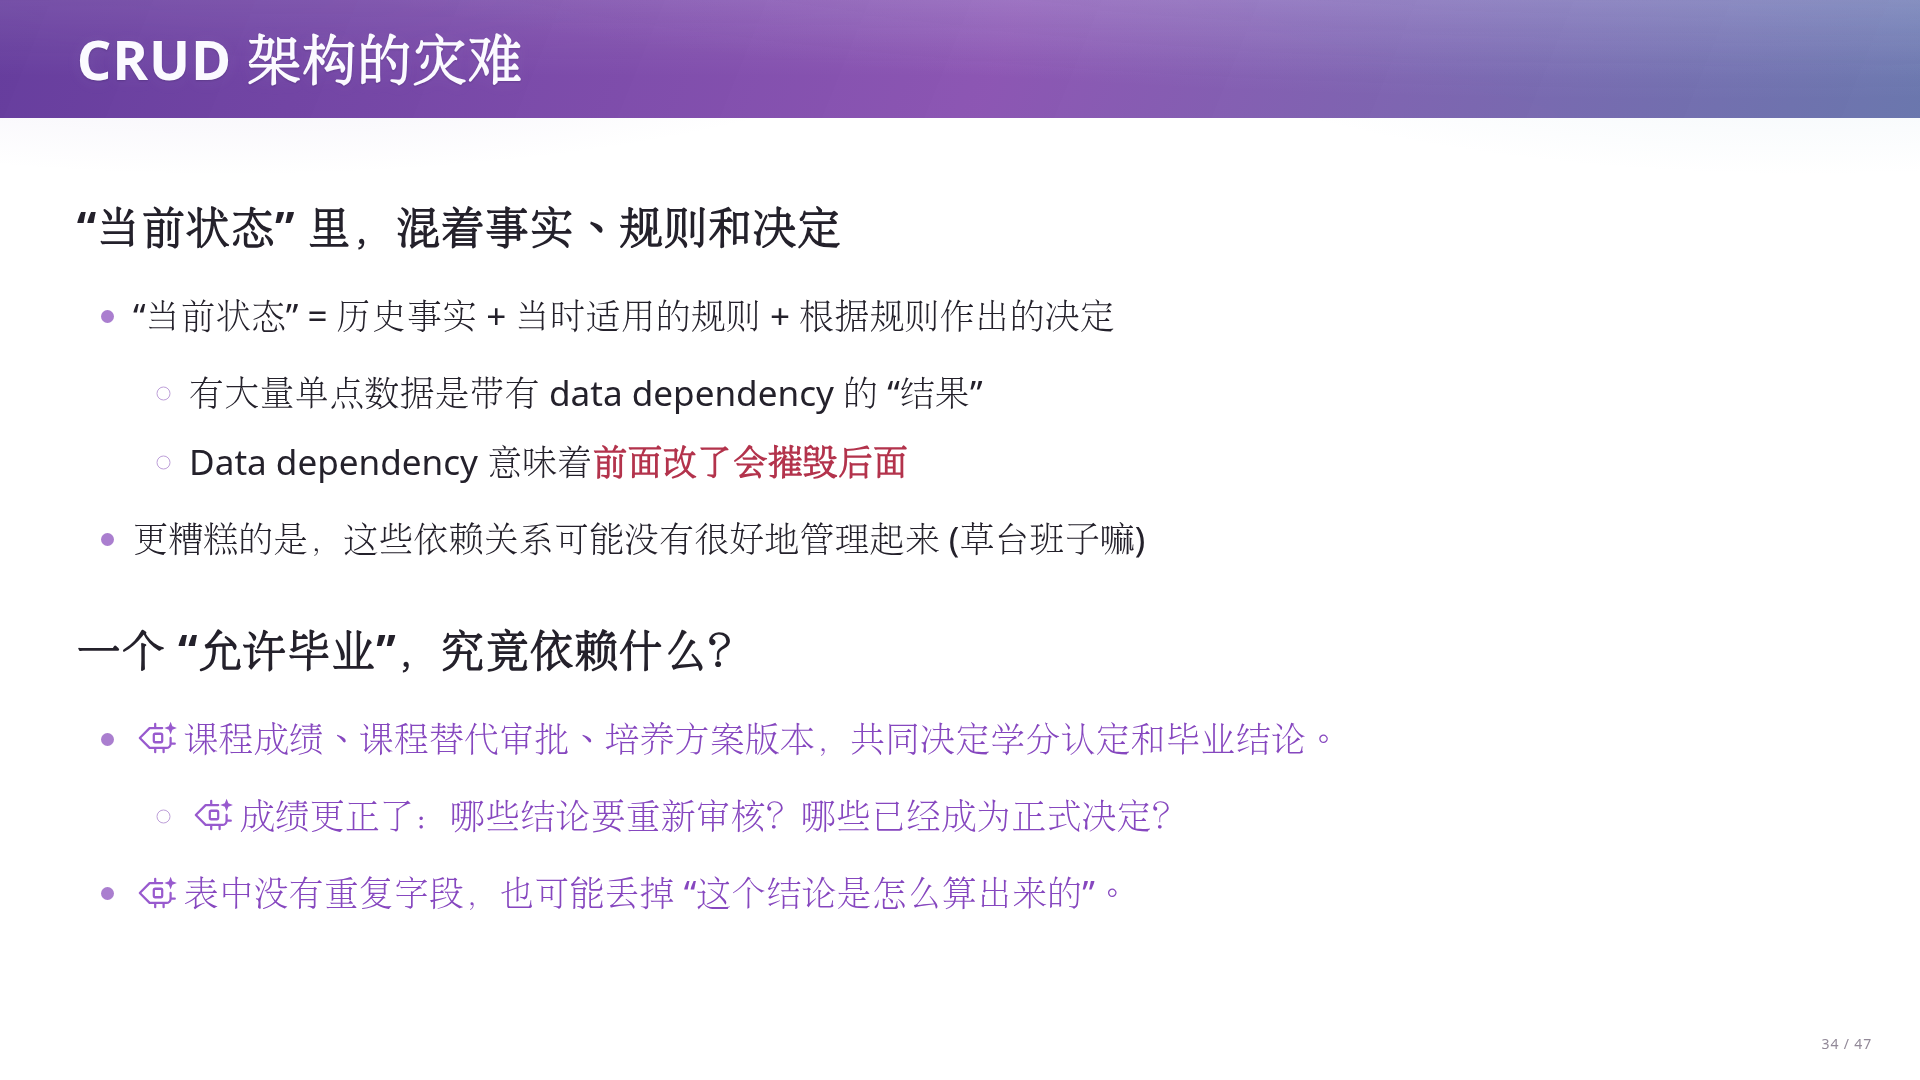
\includegraphics[width=\linewidth]{slides-images/slide-034.png}

\caption{CRUD 的结构性灾难：事实、规则与决定的混同（官方课件第 34 页）}

\end{figure}

在复杂业务下，仅覆写当前状态而不保存依据的设计之所以会带来灾难，是因为“当前状态”把“历史事实 + 当时适用的规则 + 根据规则作出的决定”压缩成了一个结果值。例如“允许毕业”这一结论，同时依赖学生的课程成绩、课程替代审批和所适用的培养方案版本。在这类状态表中，大量单点数据都是带有数据依赖的推导结果；一旦上游依赖项发生变动（如某门课成绩更正），后续的一连串结论就会受到冲击，而只存结果值的表结构却没有保存这个结论当初是怎么算出来的。

即使表结构完全符合数据库范式、没有任何重复列，这种跨表、跨时间的推导依赖依然客观存在。当一位学生的缓考成绩补录或旧成绩更正后，系统面临一连串棘手问题：哪些学分认定需要自动重算？哪些毕业审核结论需要触发复核？如果学位证书已经正式发放，历史决定还能不能被新算出的布尔值直接覆盖？只覆写当前结果而不记录依赖依据，会让系统难以回答这些问题。

\subsection{有损投影与数据黑洞：当系统外的事情先行发生}

如果所有业务都严格按照代码预设的规则在系统内部流转，或许我们还可以通过定期全量重算来维持状态一致。但现实世界的运转真的会等待软件建模完成吗？当线下政策调整或紧急特批先于系统更新发生时，只存当前状态快照的设计会遭遇怎样的冲击？这触及了软件作为“现实过程有损投影”的困境。

\begin{figure}[H]\centering


\includegraphics[width=\linewidth]{slides-images/slide-035.png}

\caption{有损投影与数据黑洞：当系统外的事情先行发生（官方课件第 35 页）}

\end{figure}

课件提出了一个关键判断：软件只是现实过程在信息世界中的有损投影。许多事情在系统之外已经发生——政策已经更新、院系领导已经签字批准某位特殊情况的学生毕业，但教务系统还没来得及开发出表达该规则的功能。为了不耽误学生当天毕业，工程师往往只能在数据库里直接执行修改（Hack），把状态强行改为满足毕业条件。日积月累，系统中沉积了大量不一致的数据，最终变成无法解释的黑洞。

课堂上老师还举了一个身边的例子：开学第一周仙林教学楼装修无法使用，线下临时人工协调换了教室，但系统模型根本来不及反映这种临时变更。同样，在毕业审核中，如果工程师救火后只留下一个冷冰冰的 \texttt{can\_graduate = true}，几个月后没人能分清这究竟是正常审核通过、正式领导特批，还是当年救火时的误操作。讲义强调，必须把“谁批准了哪项豁免、适用于谁、依据什么”作为正式业务数据记录下来，再由审批产生决定。

\subsection{语义漂移的冲击：“南大没系啦”引发的建模难题}

除了业务规则和线下特批，系统中最基础的实体定义和需求语义本身也会随时间发生漂移。当现实中的组织机构发生调整时，把无版本历史的状态表当作唯一事实来源（Single Point of Truth）的设计会面临怎样的震荡？我们以南京大学的院系调整为例，来看组织标识符的两难问题。

\begin{figure}[H]\centering


\includegraphics[width=\linewidth]{slides-images/slide-036.png}

\caption{语义漂移的冲击：“南大没系啦”引发的建模难题（官方课件第 36 页）}

\end{figure}

课件以“南大没系啦”（计算机系正式变更为计算机学院）为例，展示了需求语义变化对教务系统的冲击。面对这一现实变更，数据库架构师立即面临一个棘手抉择：代表院系的标识符 \texttt{dept\_id}，究竟应该沿用旧的，还是新开一个？这一追问揭示出，平时被我们混为一谈的一个字段，背后其实包含着“组织的名字”“组织的身份”和“当时的隶属关系”三件截然不同的事情。

在简单 CRUD 表设计中，开发者往往用一张 \texttt{department} 表存放 \texttt{dept\_id} 和 \texttt{dept\_name}，并在学生表、课程表中用外键指向 \texttt{dept\_id}。平时院系稳定时，这三件事合一没有任何异样；可一旦发生“撤系建院”或院系拆分合并，原本单一的当前状态表就再也无法同时承载历史真实性与现实业务的连续性了。

\subsection{沿用旧 ID 还是新建 ID？拆解身份、属性与隶属关系}

面对“计算机系变成计算机学院”，直接改名和新建记录这两种直观做法，各自会引发什么连锁反应？为什么说无论选哪一种，都是在对业务语义作出承诺？下面对比这两种简单做法的弊端，并给出区分身份、属性有效期的建模方案。

\begin{figure}[H]\centering

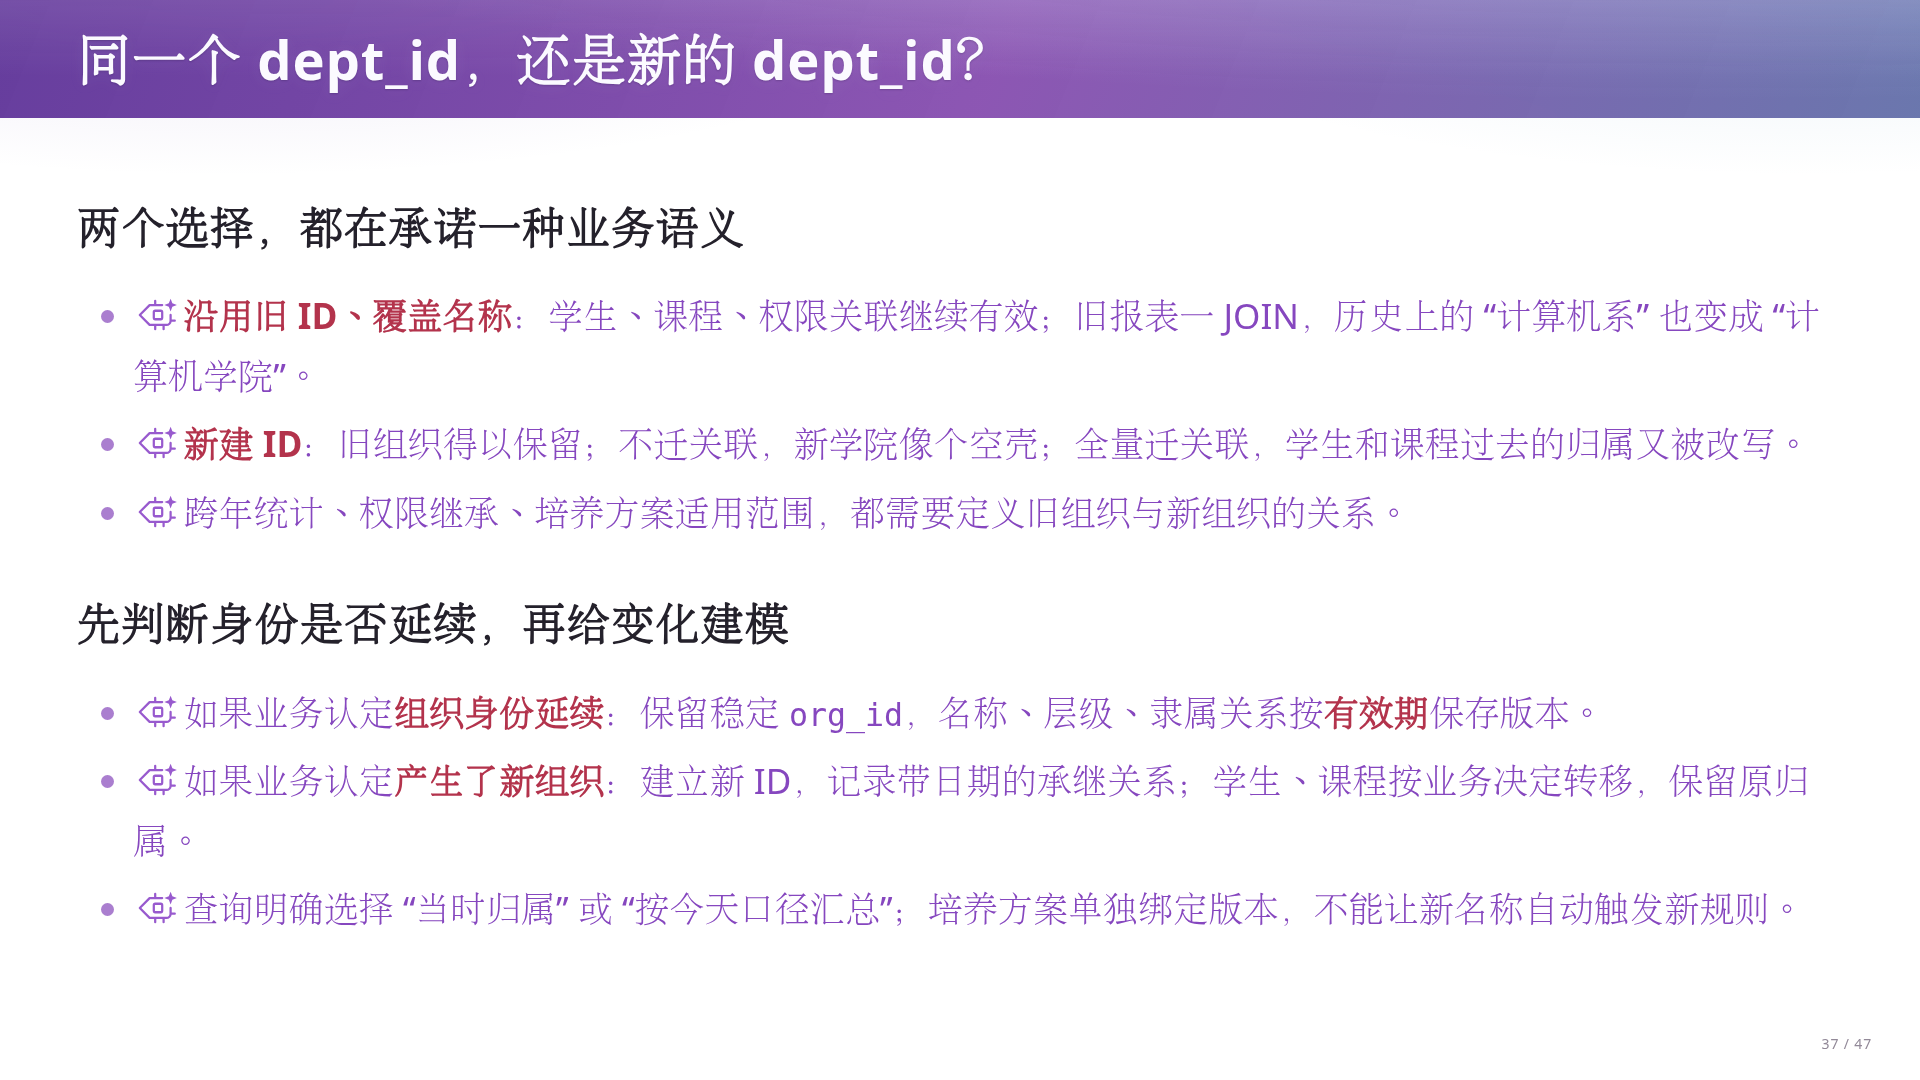
\includegraphics[width=\linewidth]{slides-images/slide-037.png}

\caption{沿用旧 ID 还是新建 ID？拆解身份、属性与隶属关系（官方课件第 37 页）}

\end{figure}

课件深入剖析了两种选择的后果：若沿用旧 ID 并直接覆盖名称，现有的学生、课程和权限关联虽能继续工作，但查询历史报表时一旦连接到当前组织表，过去毕业于“计算机系”的记录也会被篡改成“计算机学院”；若新建 ID，旧组织虽得以保留，但如果不迁移关联，新学院就成了没有学生和课程的空壳，而全量迁移关联又会抹掉学生和课程过去的归属。因此必须先由业务判断组织身份是否延续：若身份延续，则保留稳定 \texttt{org\_id}，将名称、层级等属性按有效期保存版本；若产生了新组织，则建立新 ID 并记录带日期的承继关系。

讲义进一步提醒，把组织身份、时效属性与隶属关系拆开后，查询端也必须明确统计口径：打印2011届毕业证明时，应按毕业当时的组织版本输出“计算机系”；做今日全院师资汇总时，则按当前组织结构归并。同时，培养方案必须绑定各自独立的版本号，绝不能因为院系换了名称或 ID，就让学生自动触发并适用另一套毕业要求。

\subsection{历史无法凭空修补：复杂业务系统的长期护城河}

当一个只覆写当前状态、未留存决策依据的教务系统已经在线运行多年、积累了大量历史改动与人工补丁后，我们能否轻易用 AI 重写代码并完成数据库迁移？本节作为第五章的收束，探讨系统运行后的高昂修改代价，以及历史依据对于企业级软件的真正价值。

\begin{figure}[H]\centering


\includegraphics[width=\linewidth]{slides-images/slide-038.png}

\caption{历史无法凭空修补：复杂业务系统的长期护城河（官方课件第 38 页）}

\end{figure}

课件总结道，系统一旦跑起来，修改的代价就极其高昂。代码固然可以推倒重写，但已经丢失的历史依据却无法凭空补出来。在进行数据库迁移或业务逻辑重写时，面对库里大量无法解释的不一致数据——比如同一个“已毕业”标记，可能来自正常审核、人工特批或某次紧急救火——如果没有保存当初的决策依据，即便是最强大的 AI 也推不回原来的业务含义。这也正是 ERP（Enterprise Resource Planning，企业资源计划系统）等大型业务系统的护城河所在。

课堂上老师分享了一个真实经历：早年研究生院曾委托某团队用传统 CRUD 架构定制开发了一套教务系统，起初运行尚可，但随后几年遇上研究生大规模扩招、培养类型增加与管理规则频繁调整，系统在不断打补丁和改库中逐渐演变为难以维护的遗留系统，最终只能废弃并替换为专业厂商长期维护的系统。既然只存当前状态会让系统走入死胡同，下一章我们就将探讨如何通过事件溯源（Event Sourcing）、CQRS 与领域驱动设计（DDD），把历史与依赖变成程序中的一等公民。

\begin{importantbox}{软件是现实过程的有损投影}

现实世界的业务流转永远比软件模型更丰富、更紧迫。线下政策调整、院系领导特批、甚至开学第一周因教学楼装修临时调换教室，往往在系统具备相应表达能力之前就已经发生。如果架构不为“例外审批”和“带依据的豁免”提供显式建模入口，迫使工程师直接修改数据库字段救火，那么软件就会丢失关键的因果链条，退化为无法审计、无法迁移的数据黑洞。

\end{importantbox}

\begin{knowledgebox}{课堂案例：为什么旧系统难以承受规则演进}

课堂讲述了研究生院早期定制教务系统的兴衰史：一套价值二三十万元的典型 CRUD 系统，在面对研究生扩招、新增培养类别及毕业要求调整时，由于每次规则变更都需要直接修改状态表结构与耦合在一起的查询逻辑，历史数据与新规则不断冲突，最终演变成无人敢动的遗留系统。理解并承接几十年的政策变迁与历史数据包袱，正是大型教务与 ERP 系统真正的工程壁垒。

\end{knowledgebox}

\begin{warningbox}{切勿全盘否定 CRUD 或给出非黑即白的 ID 方案}

需要明确的是，前文剖析的是“只原地覆写当前结果、不保存历史与推导依据”的建模方式（诚然，关系型 CRUD 系统也可以额外设计审计表、历史版本表来显式保存依据）；对于无需还原跨期推导过程的基础信息维护，直接读写当前状态的 CRUD 依然简单高效。同样，在面对“系改院”问题时，不能简单断言“绝对不能改 ID”或“必须新建 ID”，而必须依据业务上认定“组织身份延续（保留 ID、属性按有效期版本化）”还是“新设组织（新建 ID、记录带日期的承继关系）”来建模。

\end{warningbox}

\par\needspace{5\baselineskip}\textbf{术语消化：CRUD 状态快照架构的核心概念与演化困境消化表}

\begin{center}\small\begin{tabularx}{\linewidth}{YYY}

\toprule

术语或概念 & 解决的问题或扮演角色 & 内在机制与课程主线的关系\\\midrule

基于当前状态快照的 CRUD 建模 & 提供直观的当前状态维护与基础信息增删改查 & 仅用当前状态快照描述世界，若每次操作直接原地覆盖旧值而不存历史表与依据，虽在简单维护中高效，却会抹去跨期业务的推导过程。\\[3pt]

数据库范式（Normal Form） & 消除关系表内的字段重复与更新不一致异常 & 通过表分解与外键引用（如用学号代替重复存姓名）减少表内冗余，但无法自动保存跨业务规则计算的因果依赖。\\[3pt]

有损投影（Lossy Projection） & 揭示信息系统状态与物理世界真实过程之间的差距 & 将“历史事实+适用规则+审批决定”压缩成单个布尔或状态字段，导致线下特批与工程师救火改库后丢失业务依据。\\[3pt]

组织身份与属性版本化（org\_id \& 有效期） & 应对“撤系建院”等组织架构调整引发的语义漂移 & 把稳定的组织身份标识、按有效期版本化的名称层级属性、以及特定时刻的师生隶属关系拆分为三件事独立建模。\\[3pt]

\bottomrule\end{tabularx}\end{center}

\needspace{7\baselineskip}\subsection{本章小结}

本章以五十万行教务系统为例，剖析了用 AI 快速生成大文件单体及采用传统 CRUD 架构的深层局限。

尽管数据库范式能消除表内冗余，但仅原地覆写当前状态而不保存依据的 CRUD 建模将“\textbf{历史事实、适用规则与审批决定}”压缩为单一快照，在线下特批改库与“撤系建院”等语义漂移冲击下会沦为难以解释的数据黑洞，这迫使我们寻找能\textbf{显式保存历史与依赖}的架构方案。

\needspace{8\baselineskip}\section{第六章 把历史与依赖变成一等公民：事件溯源与重放语义}

上一章我们看到，CRUD架构将历史事实、适用规则与推理结论全部压缩进数据库的当前状态快照里。一旦业务规则发生变更，或者组织架构像“计算机系改名为计算机学院”那样发生语义漂移，原地覆盖就会抹除历史依据，让数据变成无法解释的黑洞。既然未管理的数据依赖与丢失的历史是痛苦的根源，我们能否跳出只存当前状态的思维定式，把操作历史与依赖关系直接提升为程序中的一等公民？本章将引入事件溯源（Event Sourcing），探讨如何从已接受的业务事件序列中构建系统状态，并厘清历史重放（Replay）在工程落地时必须严守的语义边界。

\subsection{把依赖与历史提升为一等公民}

在传统数据库设计中，我们习惯直接覆写字段来反映最新情况，却把导致变化的业务过程丢弃在数据库之外。我们需要思考：数据结构除了记录“此刻是什么样”，能否直接记录“过去发生过什么”？当我们将状态变化的历史与依赖显式保存下来时，系统的状态机语义会发生怎样的转换？

\begin{figure}[H]\centering

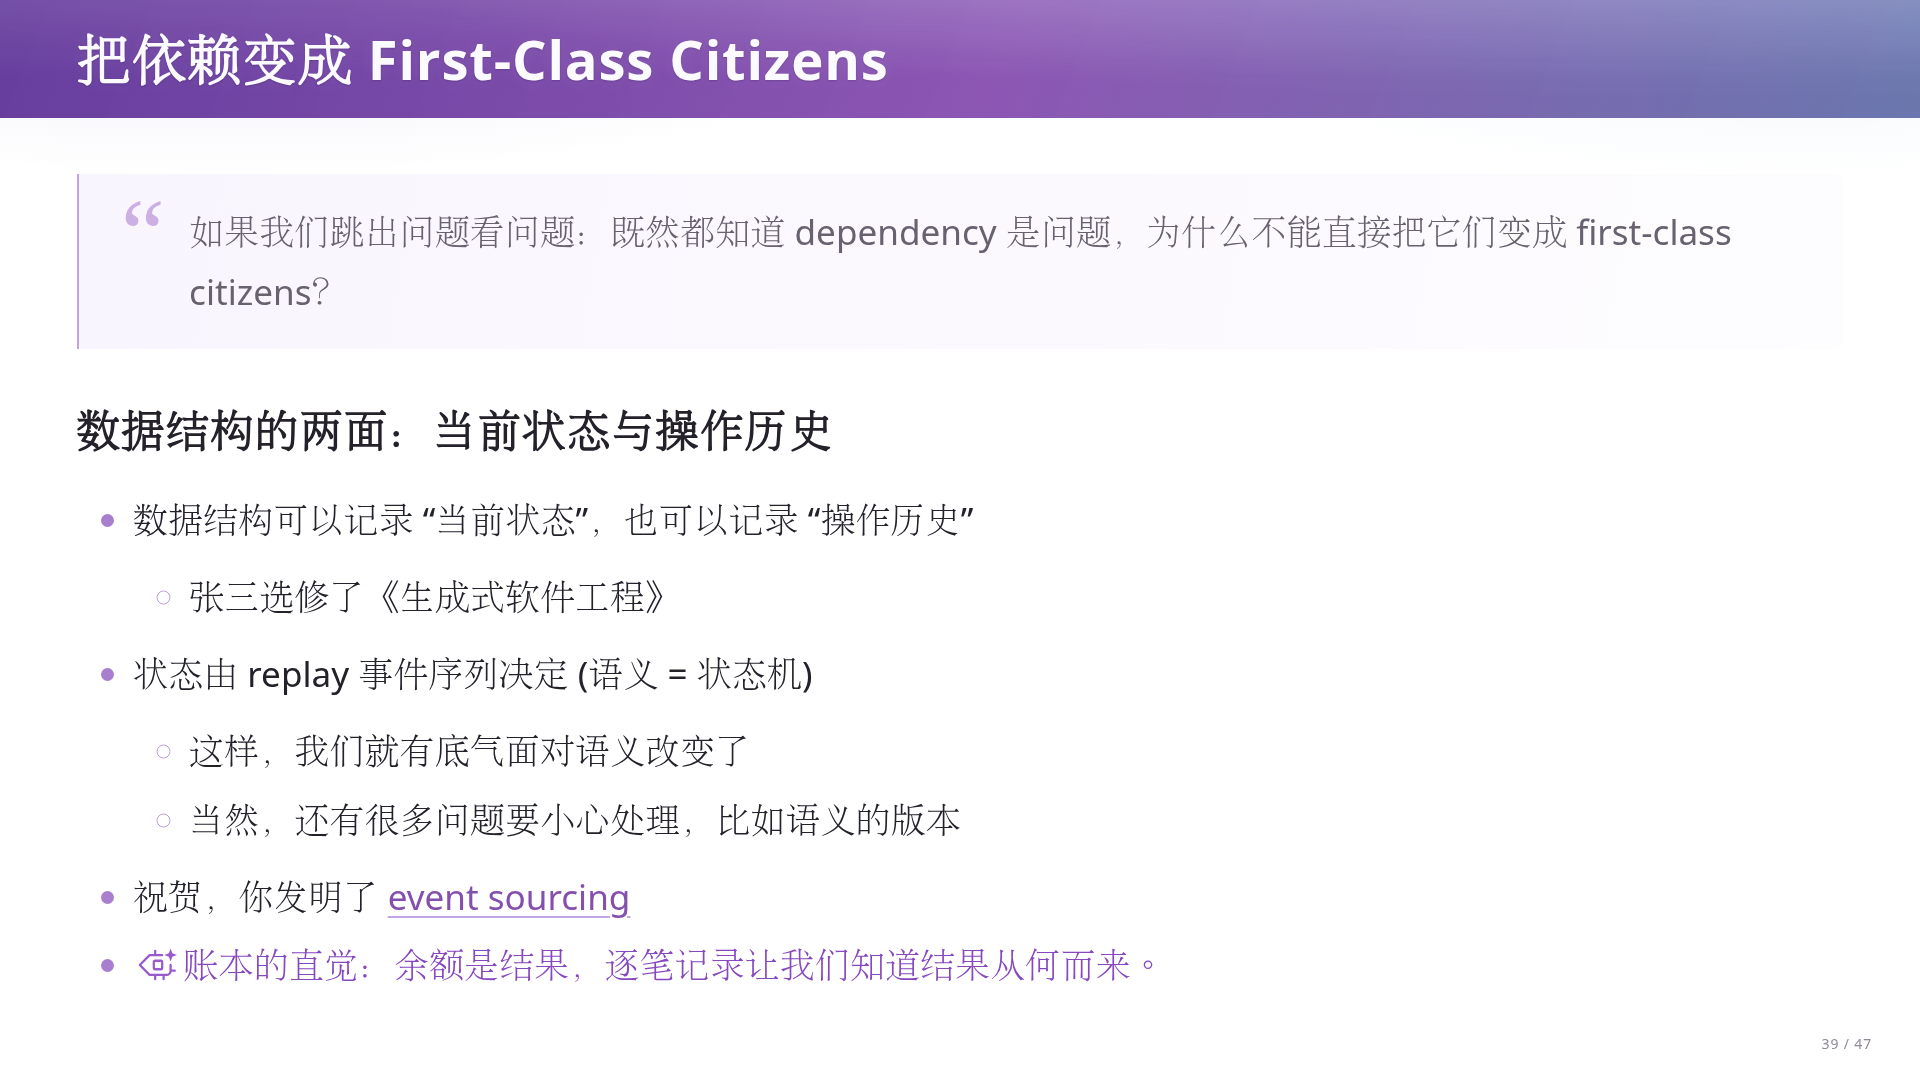
\includegraphics[width=\linewidth]{slides-images/slide-039.png}

\caption{把依赖与历史提升为一等公民（官方课件第 39 页）}

\end{figure}

由此引出了把依赖与历史变成一等公民（First-Class Citizens，即编程语言或系统中可以明确表示、传递、保存和处理的对象）的架构思路。

观察数据结构的两个侧面：如果只保存“张三选修了《生成式软件工程》”，这只是\textbf{当前状态}；如果保存“张三的选课申请已被接受”，以及后续是否退选、是否再次选入的操作序列，就是保存\textbf{操作历史}。

在事件溯源（Event Sourcing）模式下，状态不再通过原地修改维护，而是由重放（Replay，即从初始状态或快照出发按序重新应用已有事件）事件序列来决定。

这就好比日常的银行账本：账户余额只是当前计算出的结果，而逐笔收支记录才能解释余额为何变成今天这个数字。

课堂上老师联系了三门基础课的直觉来打通这一概念：数据结构课中的可持久化数据结构（Persistent Data Structure）在修改树节点时保留原节点、只沿修改路径创建新版本；数据库与操作系统课中的预写日志（Write-Ahead Log, WAL）在修改数据页前先把变更写入日志；以及 Git 版本控制在每次提交时逻辑上记录项目快照与父提交指针（底层可通过快照比对计算 diff，或在 packfile 存储中采用 delta 压缩）。例如早期教务系统若未设计“复学”功能，在CRUD模式下学生退学就直接删表记录，日后想复学时关联早已丢失；若完整记录了“入学、选课、退学、复学”等不可篡改的事实，即使未来增加复学规则或遇到院系改名，也能截取相应时间点的历史回放出当时的真实状态。

\subsection{从已接受事实构建状态与投影}

理解了账本式的事件记录思想后，我们需要看清事件溯源在教务系统中具体怎样运转。观察事件溯源的架构流向，我们需要看清按时间排列的业务事件如何生成不同的业务视图，并思考：如果每次查询课表都要把学生从入学以来的所有事件重算一遍，系统性能该如何保障？

\begin{figure}[H]\centering

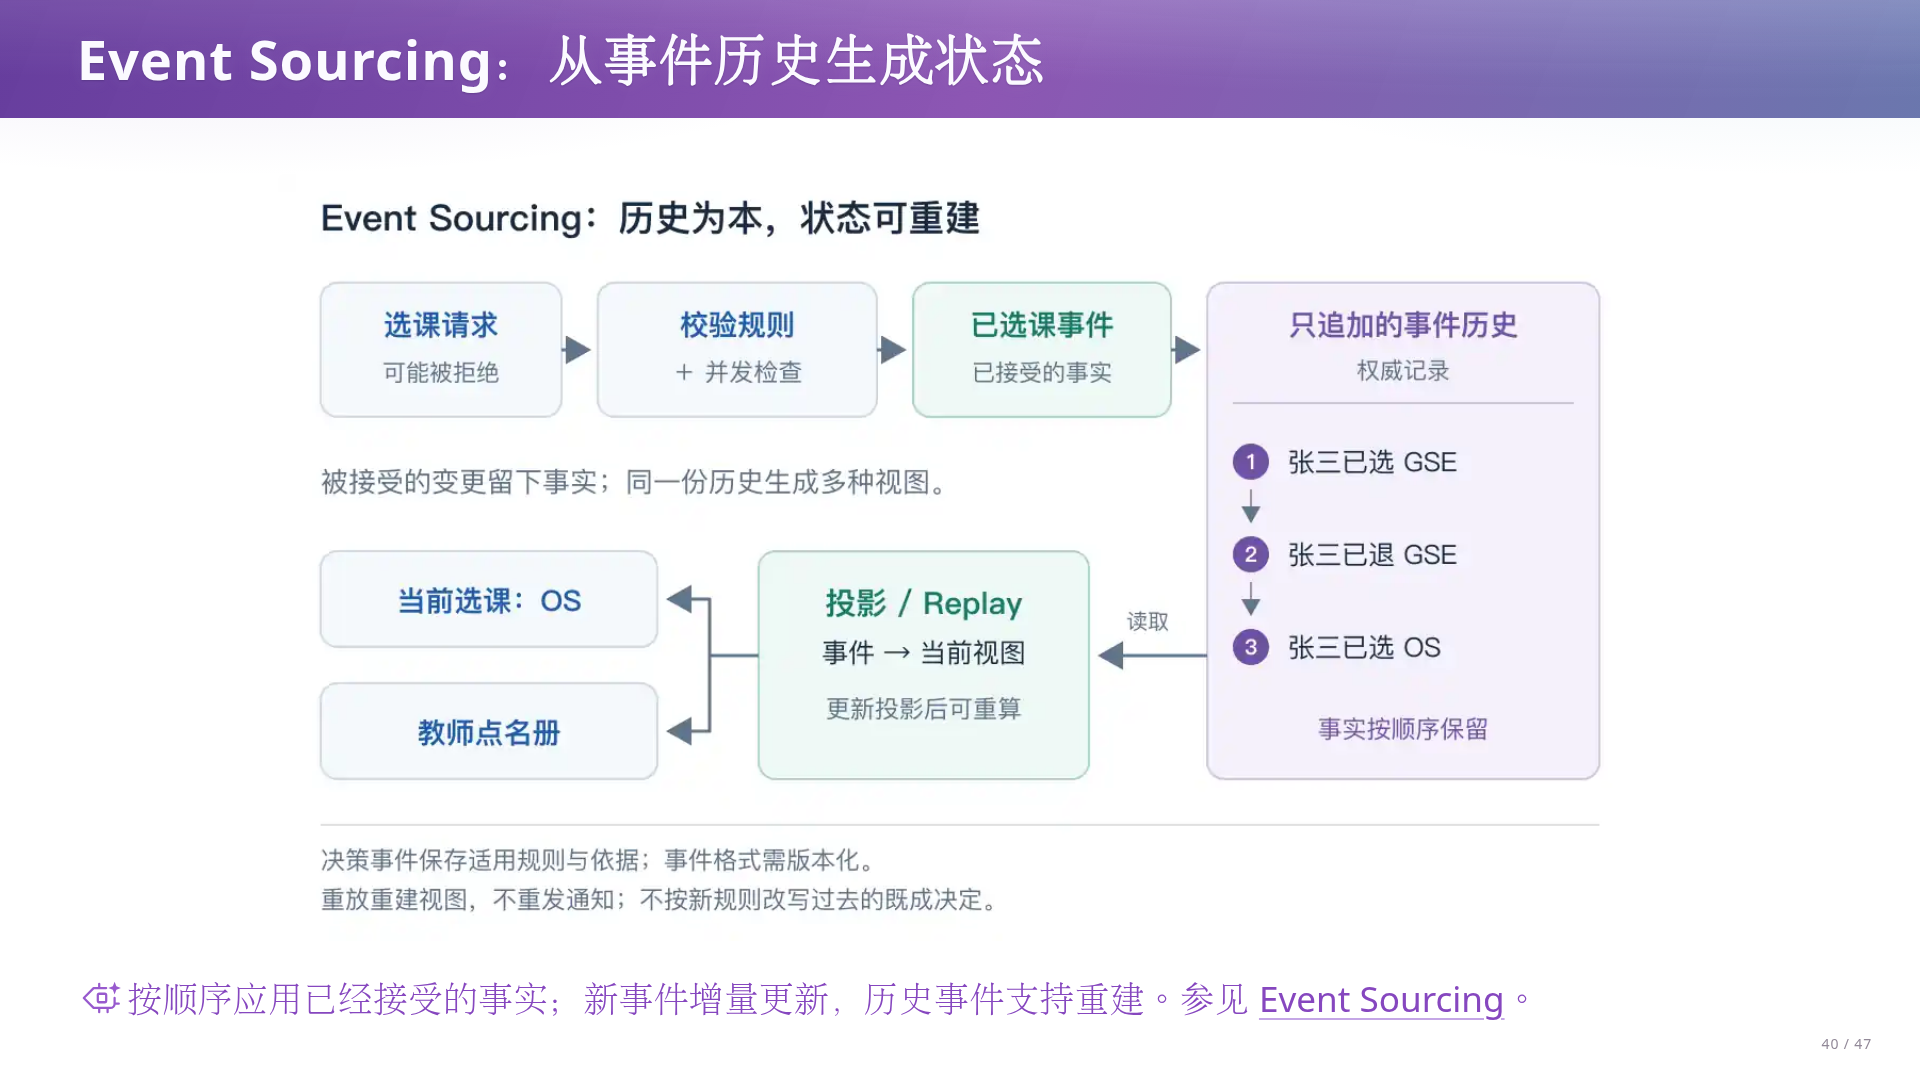
\includegraphics[width=\linewidth]{slides-images/slide-040.png}

\caption{从已接受事实构建状态与投影（官方课件第 40 页）}

\end{figure}

事件溯源从事件历史生成状态的完整链路是：在教务系统中，被系统校验并接受的业务事实被依次追加记录下来，例如“选课已接受”“成绩已登记”“课程替代已批准”“毕业审核已完成”等。把这些事件序列转换成某种当前状态或专用查询结果的过程，称为投影（Projection）。如图所示，同一份底层已接受的业务事件流，可以通过不同的投影逻辑，分别构建出面向学生的当前选课课表和面向教师的课程点名册。为了避免每次查询都从头计算，系统在日常运行中会维护当前查询结果，当新事件到来时只做增量更新；只有需要修正视图或迁移逻辑时，才利用历史事件进行重建。

讲义与课堂特别回应了关于重放性能的常见顾虑：保存完整历史绝不等于每次打开网页都要从大一入学第一天开始重放所有事件。工程实现上，除了新事件的增量更新外，还可以定期为状态打下带有明确事件位置标记的快照（Snapshot）。当需要重建状态时，只需从最近的快照加载基线，再接着向后重放快照之后的增量事件即可。不过讲义提醒，单纯的事件序列只记录了“发生了哪些变化”，若要回答某个毕业结论为何成立，还必须在事件和决定中显式连接数据依赖。

\subsection{重放的边界：恢复历史与按新规则重算}

拥有了事件序列和重放机制，很容易产生一种幻觉：是不是只要保存了事件，以后无论培养方案怎么改，随便重放一下就能解决所有历史遗留问题？为此，我们必须严格区分“恢复历史”与“按新规则重新计算”这两件完全不同的事，并明确让历史真正可解释、可安全重放的四项工程条件。

\begin{figure}[H]\centering

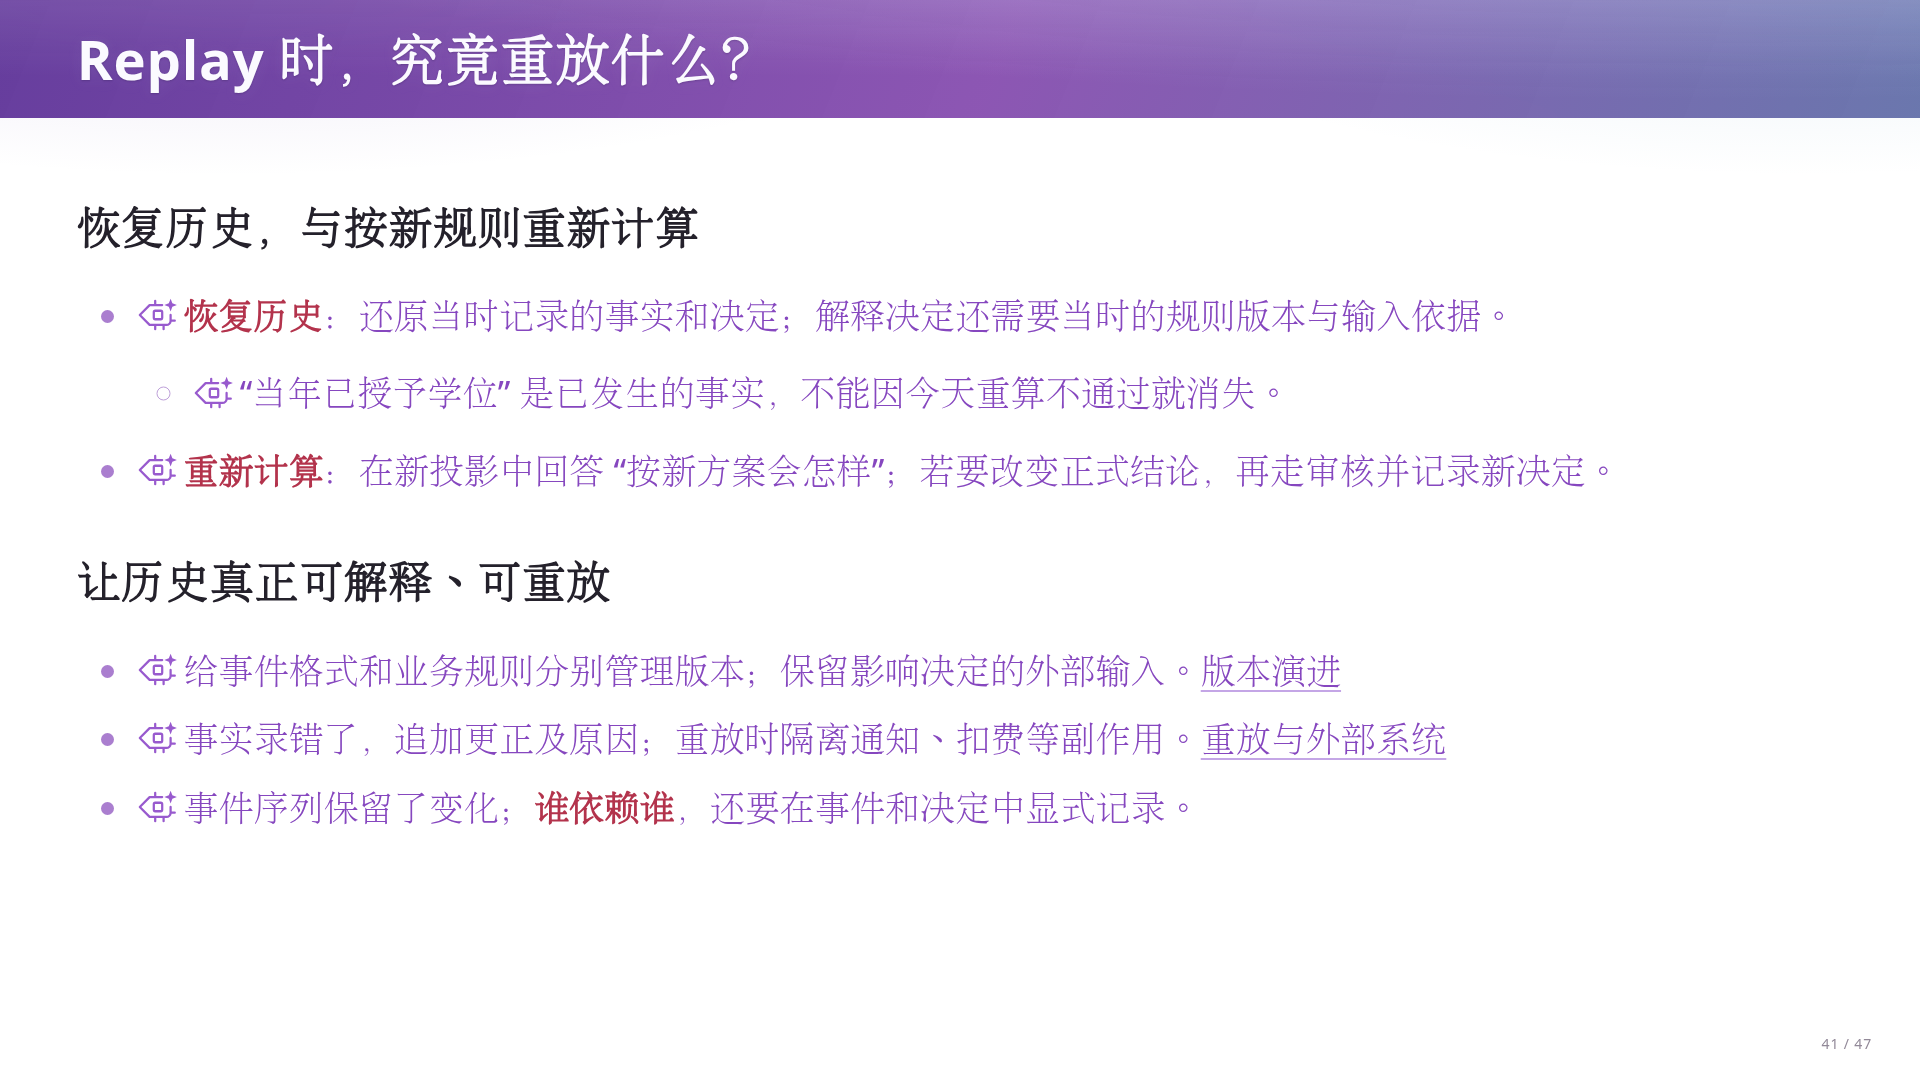
\includegraphics[width=\linewidth]{slides-images/slide-041.png}

\caption{重放的边界：恢复历史与按新规则重算（官方课件第 41 页）}

\end{figure}

重放（Replay）时必须严守两条核心语义边界。首先必须区分两类问题：第一类是“恢复历史”，目标是还原当时发生了什么、为什么作出该决定，这不仅需要当时的事实事件，还必须绑定当时的规则版本与输入依据；例如“当年已授予学位”是既成历史事实，绝不能因为今天用新规则重算不达标，就让已授予学位的事实从历史中抹除。第二类是“重新计算”，即在新投影中回答“如果按今天的新方案审核会得到什么结果”，若业务上确实要更改正式结论，必须走复核流程并追加记录新的决定事件。其次，为了让历史真正可解释、可重放，工程上必须做到：分别管理事件格式与业务规则的版本；事实录错时通过追加更正事件及原因来修正，而非直接篡改原记录；重放时严格隔离发送通知短信、扣费等外部副作用；并显式记录决定背后的外部输入与“谁依赖谁”的依赖关系。

为什么要把外部输入和副作用隔离看得如此重要？设想教务系统管理员为了重建一张选课统计视图而触发了历史事件重放，如果重放代码里直接混杂着调用短信网关或财务扣款接口，全校学生就会在半夜收到几十条重复的选课确认短信甚至被重复扣费。同理，如果当年某项审批依赖了外部学籍库在那一刻返回的查询结果，重放时若再去实时请求外部接口，拿到的就是今天的值而非当年的历史依据。至此我们看到，事件溯源解决了历史保存问题，而在系统入口如何分离“做决定的写操作”与“看结果的读查询”，正是下一章CQRS架构要解决的主题。

\begin{importantbox}{区分“恢复历史”与“按新规则重算”}

在事件溯源系统中，重放事件流不能混为一谈。回答“当年为什么批准该学生毕业”，必须使用当时的事件、当时适用的培养方案规则版本以及当时的外部输入快照，这是恢复历史事实；回答“如果用2026年新方案审核该学生会怎样”，则是用新规则对历史事件做一次新的候选投影。新投影的计算结果只能作为复核参考，绝不能自动覆盖或抹去历史上已经正式发布的学位授予决定。

\end{importantbox}

\begin{knowledgebox}{可持久化数据结构与账本直觉}

理解事件溯源不需要死记复杂的分布式框架，可以从几个基础机制的对比出发：会计账本中，账户余额只是当前聚合结果，逐笔收支流水才是事实来源；可持久化树（Persistent Tree）在修改时不原地覆写旧节点，而是共享未变子树、沿修改路径创建新节点以保留历史版本；数据库的预写日志（WAL）要求变更日志先于数据页落盘以保障崩溃恢复（数据页本身仍会被更新）；而事件溯源则将已接受的业务领域事件作为追加日志保存。需要注意，单个当前状态快照无法倒推出历史演进过程，纯状态差值（diff）也无法自动还原业务意图，只有显式保存带上下文的业务事件与决策依据，系统才具备回溯与解释过去的能力。

\end{knowledgebox}

\begin{warningbox}{重放的三大工程禁忌：篡改历史、丢失规则版本与触发外部副作用}

落地事件溯源时有三个常见陷阱：第一，切勿以为只存事件序列就能自动解释一切，若不保存每次决定所依赖的规则版本和输入依据，重放时依然算不出当年的逻辑；第二，发现历史事实录入错误时，严禁直接进数据库UPDATE或DELETE旧事件，必须追加一条带有原因的更正或补偿事件；第三，重放路径必须成为纯计算过程，严禁在重建投影视图时再次触发发短信、发邮件或财务扣款等外部世界副作用。

\end{warningbox}

\par\needspace{5\baselineskip}\textbf{术语消化：事件溯源与历史重放核心术语消化}

\begin{center}\small\begin{tabularx}{\linewidth}{YYY}

\toprule

术语 & 解决的问题 & 机制与课程关系\\\midrule

事件溯源（Event Sourcing） & 避免CRUD原地覆写导致历史过程与决策依据丢失 & 将系统接受的状态变化保存为只追加的事件序列，通过按序应用事件来重建当前状态\\[3pt]

投影（Projection） & 从单一事件流构造满足不同角色需求的查询视图 & 将事件序列按特定业务规则转换为学生课表、教师点名册或审核统计表等派生状态\\[3pt]

重放（Replay） & 在视图损坏、新增查询口径或回溯历史时重建状态 & 从初始状态或指定位置的快照（Snapshot）出发，重新按序应用已有事件，同时隔离外部副作用\\[3pt]

补偿/更正事件（Compensating Event） & 在不篡改历史记录的前提下修正录入错误的事实 & 追加一条新的更正事件并记录修改原因与原事件关联，保留完整的错误发生与修正轨迹\\[3pt]

\bottomrule\end{tabularx}\end{center}

\needspace{7\baselineskip}\subsection{本章小结}

本章从可持久化数据结构与账本直觉出发，介绍了如何通过\textbf{事件溯源（Event Sourcing）}将状态变化与数据依赖提升为系统的一等公民。通过记录已接受的业务事件、利用投影（Projection）与增量快照生成视图，系统得以摆脱CRUD黑洞。

在执行历史重放（Replay）时，必须严格区分“\textbf{按旧规则恢复历史}”与“\textbf{按新规则重新计算}”，分别管理事件与规则版本，采用追加更正事件处理错误，并彻底隔离短信、扣费等外部副作用。

\needspace{8\baselineskip}\section{第七章 读写分离、业务边界与渐进式架构演进}

上一章通过事件溯源把操作历史提升为一等公民，解决了状态变化如何留存与重放的问题。然而，一个五十万行规模的真实教务系统不仅要记录历史，还要在每天高频发生的操作中同时应对两类截然不同的挑战：一方面是选课冲突检查、名额争抢、学分认定与毕业审批等严密的业务决策，另一方面是面向学生、教师、教务员与财务人员的复杂多维查询。如果把做决定的约束逻辑、多方角色的查询视图以及错综复杂的业务概念全部塞进同一套数据库表结构与大文件里，系统依然会迅速腐化。本章将探讨如何结合命令与查询职责分离（CQRS）与领域驱动设计（DDD）来划分读写职责和业务边界，并讨论如何把依赖关系、双时态时间模型与渐进式换轨策略落地到正在运行的遗留系统中，让下一次需求变化有清晰的归处。

\subsection{CQRS：分离做决定的写模型与看结果的读模型}

在传统增删改查（CRUD）系统中，同一个数据模型既要承接修改状态的操作，又要应付五花八门的页面展示与报表查询。当选课校验规则越来越复杂，而学生课表、教师点名册和教务统计又要求各不相同的聚合视图时，单一模型就会顾此失彼。这就需要考虑如何将“怎样做决定”与“怎样看结果”拆分为两个独立的模型职责。

\begin{figure}[H]\centering

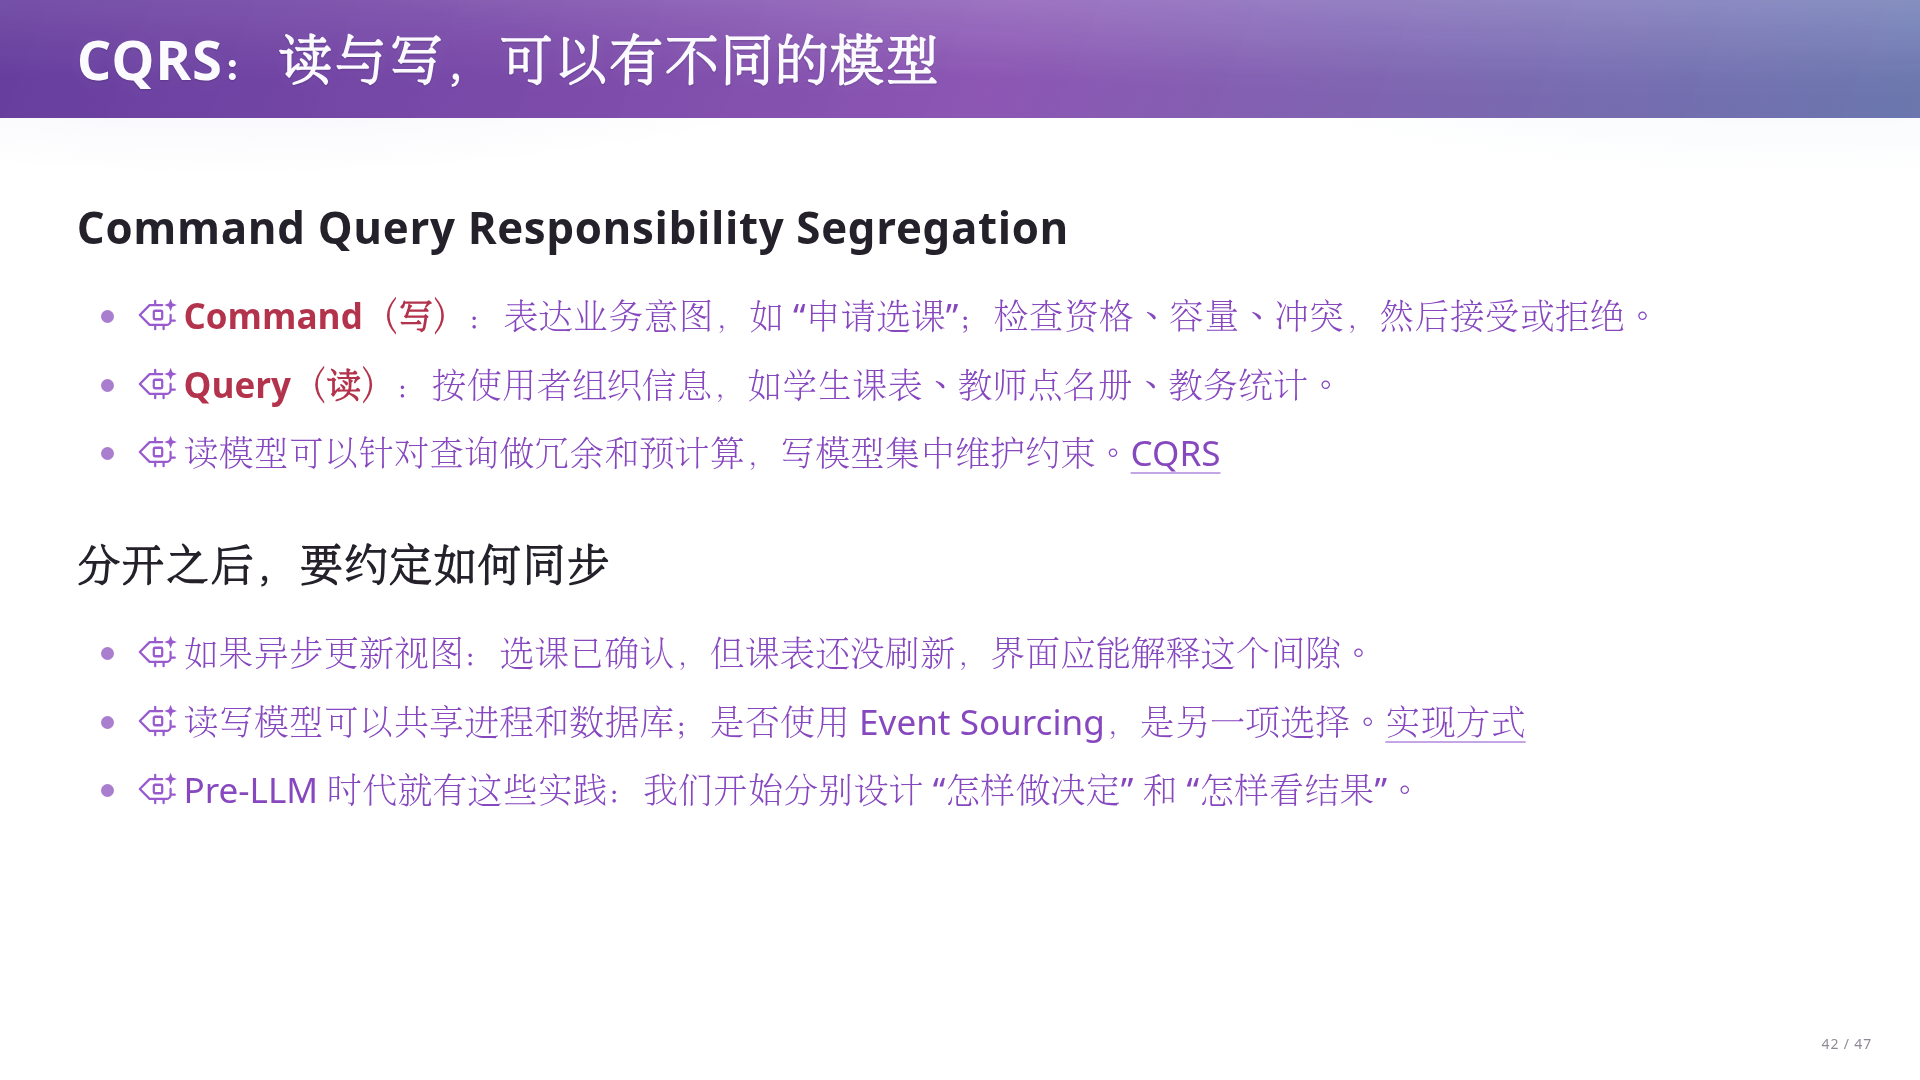
\includegraphics[width=\linewidth]{slides-images/slide-042.png}

\caption{CQRS：分离做决定的写模型与看结果的读模型（官方课件第 42 页）}

\end{figure}

这种设计就是命令与查询职责分离，即 CQRS（Command Query Responsibility Segregation，将负责接受业务修改操作的\textbf{写模型}与负责提供数据查询结果的\textbf{读模型}分别设计的架构模式）。

\begin{itemize}
\item 在写的一端，Command（命令）明确表达一个具体的业务意图，例如“申请选课”；写模型专门负责检查先修资格、课程容量与时间冲突，随后作出接受或拒绝的决定，集中维护业务约束。

\item 在读的一端，Query（查询）按不同使用者的视角组织信息，如学生课表、教师点名册和教务统计；读模型可以针对特定查询做适当的数据冗余和预计算，而不必受制于写端严密的范式结构。

\end{itemize}
两套模型分开后，必须明确约定同步方式：如果采用异步事件来更新查询视图，就可能出现选课已被写端确认、但学生课表尚未刷新的短暂时间间隙，此时前端界面必须能够明确解释这一过渡状态。

讲义特别提醒，CQRS 的核心在于拆分两类模型的职责边界，它完全可以在同一个进程、同一个关系型数据库里实现；至于底层是否进一步采用事件溯源（Event Sourcing）来保存状态变化，则是另一项正交且独立的架构选择。如果界面没有向用户解释异步刷新的短暂延迟，用户看到课表里还没有新选的课，就会误以为操作失败而反复点击提交。在理清了单个业务模块内部的读写职责分离之后，接下来的问题是：面对整个教务系统庞大的参演角色，不同业务板块之间又该如何划定概念边界？

\subsection{DDD：用业务概念与限界上下文划定软件边界}

当教务系统的功能覆盖选课、收费、成绩管理与毕业审核时，如果开发者只围绕底层数据库表名来讨论系统，或者试图设计一个无所不包的“超级学生类”去装下全校所有业务的字段与规则，代码很快就会因为概念混杂而难以理解。我们需要思考业务语言如何进入代码结构，以及同一个现实个体在不同业务边界内为何应当拥有不同的模型。

\begin{figure}[H]\centering

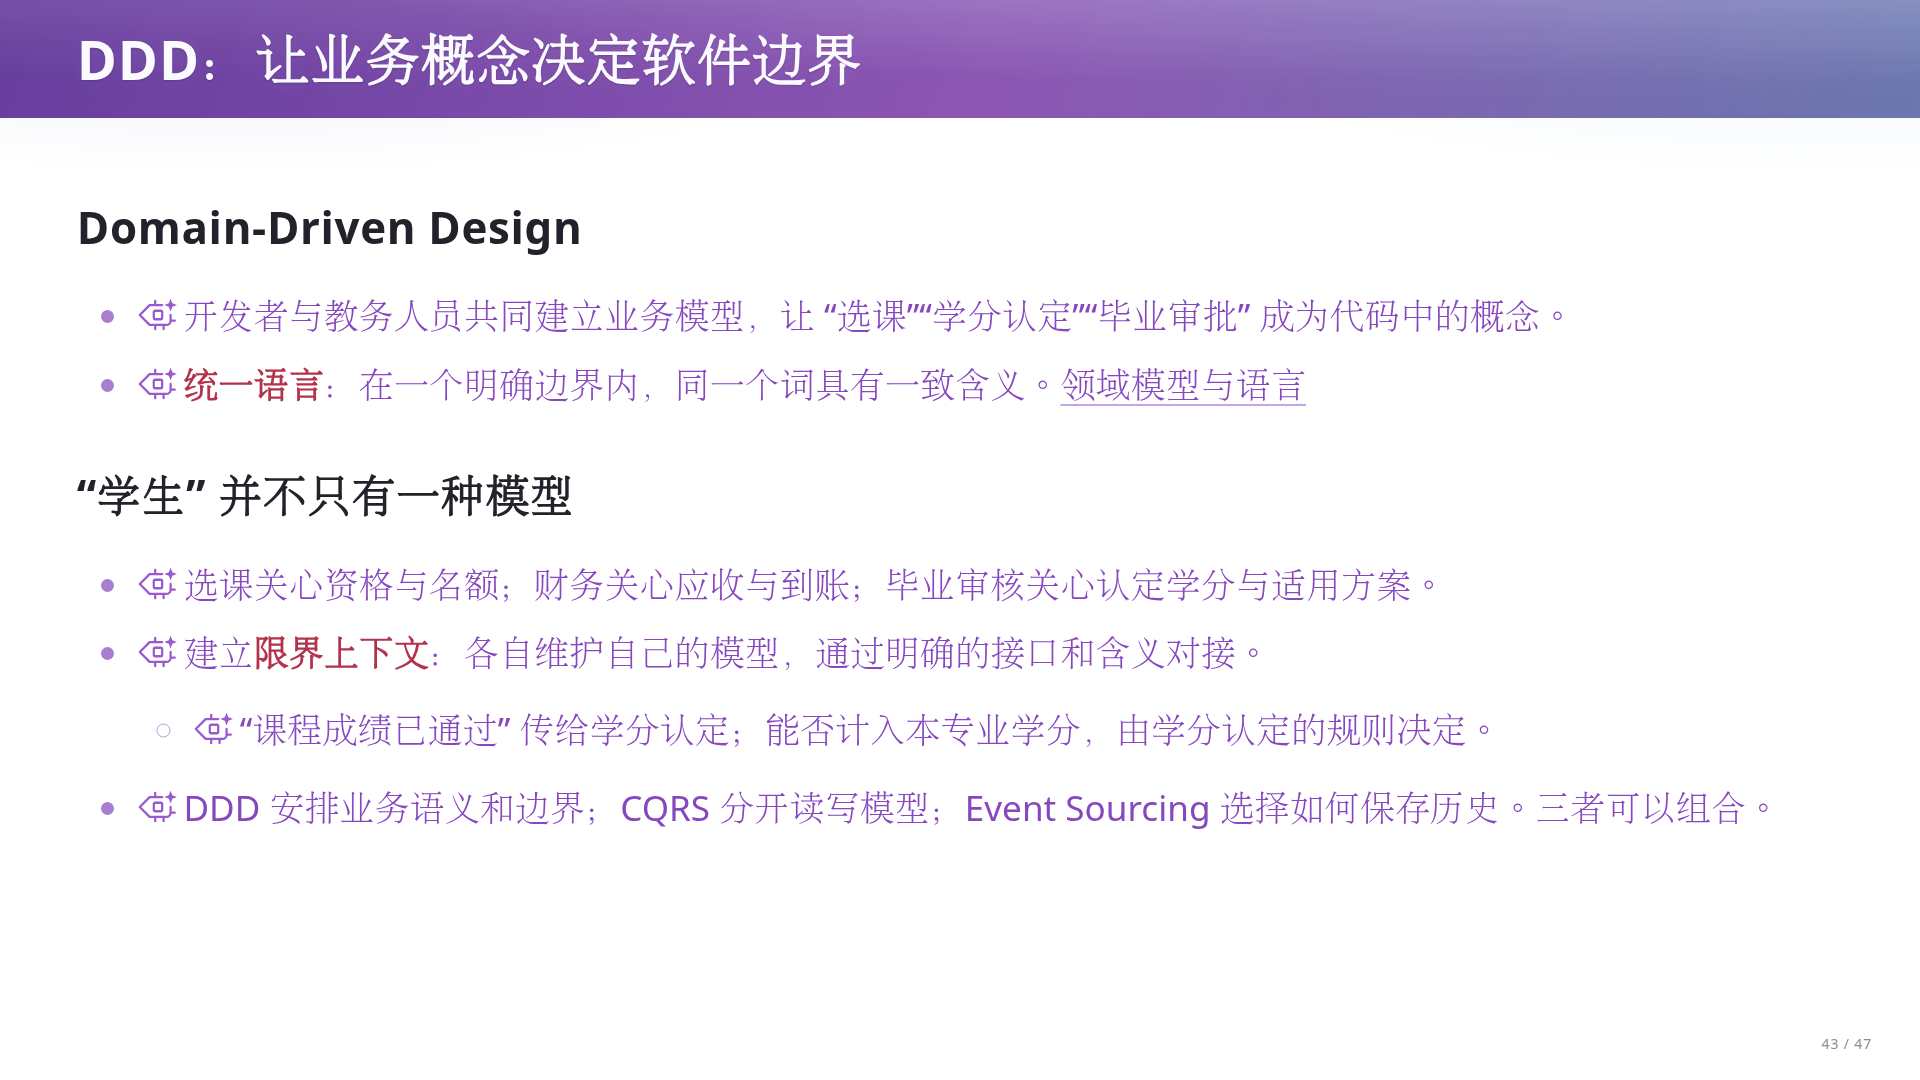
\includegraphics[width=\linewidth]{slides-images/slide-043.png}

\caption{DDD：用业务概念与限界上下文划定软件边界（官方课件第 43 页）}

\end{figure}

这正是领域驱动设计，即 DDD（Domain-Driven Design，通过开发者与业务人员共建领域模型，让核心业务概念直接决定软件结构与模块边界的设计方法）的核心思想。首先，团队需要在明确边界内建立统一语言（Ubiquitous Language，在特定业务范围内让开发者与教务人员对同一个术语保持严格一致含义的共同词汇表），让“选课”“学分认定”“毕业审批”直接成为代码中的一等概念。其次，系统通过限界上下文（Bounded Context，明确特定领域模型适用范围与语义边界的架构划分单元）避免全局大一统模型：同样谈论“学生”，选课上下文关心选课资格与剩余名额，财务上下文关心应收学费与到账状态，毕业审核上下文则关心已认定学分与适用的培养方案。各限界上下文独立维护自己的模型，并通过含义明确的接口传递信息。例如，成绩管理上下文将“课程成绩已通过”传递给学分认定上下文作为输入，但该成绩能否计入本专业毕业学分，必须由学分认定上下文根据培养方案规则独立裁决。

讲义指出，如果贪图省事，把“课程及格”和“满足毕业学分要求”直接压缩成数据库里的同一个 passed 布尔字段，将来遇到“外系交换课成绩合格但按规则不能抵扣本专业核心课学分”的情况时，系统就会陷入无法解释的自相矛盾。至此，我们可以看清三大架构思想的分工与协作关系：DDD 负责安排业务语义和模型边界，CQRS 负责分开接受操作与提供查询的职责，而事件溯源则提供保存和重建历史的底层机制。三者既可以按需独立采用，也可以组合使用。有了清晰的模型边界与读写分工，下一步就是如何把具体的数据依赖与时间维度落实到教务系统的记录结构中。

\subsection{实践落地：让审核结论携带依据与双时态历史}

在前文的 CRUD 案例中，一个孤零零的允许毕业布尔值掩盖了背后的推理过程，导致上游成绩更正或线下延期录入批件时，系统既不知道哪些历史结论已经失效，也解释不清过去某个时刻为何作出了拒绝决定。下面我们来看一条完整的毕业审核记录应当保存哪些元数据，以及如何用两个独立的时间维度消除跨期录入带来的解释困境。

\begin{figure}[H]\centering


\includegraphics[width=\linewidth]{slides-images/slide-044.png}

\caption{实践落地：让审核结论携带依据与双时态历史（官方课件第 44 页）}

\end{figure}

将规则、依赖与时间显式建模为数据，包含两项具体工程实践。第一，让每一个业务结论随身携带它的完整依据：一次毕业审核记录不再只存“通过”或“不通过”，而是显式记录输入记录的 ID 与版本号（或当时的输入快照）、所使用的培养方案规则版本、最终审核结论以及人工审批依据。这样一来，当某门课程的成绩发生更正时，系统就能顺着显式保存的结果对输入的依赖关系，精准定位所有受影响的毕业审核记录；对于已经正式发布的决定，则触发规范的复核流程。同时，由于规则独立进行了版本化管理，面对同一批学生历史事实，系统可以并行计算多个候选培养方案并直观对比结果差异。第二，引入双时态历史（Bitemporal History，同时记录现实业务发生或生效的时间与系统实际获知并录入该事实的时间的历史建模方法）。例如，一项课程豁免在 6 月 1 日正式生效，但教务员直到 6 月 3 日才将其录入系统。同时保留这两个时间戳，系统就能分别且自洽地回答两个不同维度的问题：“6 月 2 日那天该豁免在业务上是否已经生效？”（是，因为生效时间早于 6 月 2 日）以及“6 月 2 日那天系统为什么拒绝了该生的毕业申请？”（因为截至 6 月 2 日，系统尚未获知这条 6 月 3 日才录入的豁免记录）。

通过把输入版本、规则版本和双时态时间戳全部变成一等公民数据，教务系统终于告别了靠工程师直接修改数据库布尔值救火的黑洞状态。无论是事后审计为什么放行，还是追查某次自动拒绝是不是系统缺陷，都有据可查。解决了单个结论的可追溯性与时间解释之后，我们在面对高并发写入与模块划分时，还需要进一步回答：系统中哪些状态必须严格同步修改，哪些容易变化的业务决策又该如何隔离在模块边界之内？

\subsection{实践落地：划定一致性边界与模块化信息隐藏}

在引入读写分离与异步视图更新后，系统并非所有环节都能容忍“稍后一致”。如果选课抢名额时也放任并发穿插，就会造成超额选课的业务事故；反之，如果为了追求模块化而盲目把所有功能拆成分布式微服务，又会引入原本不必要的网络与运维复杂度。我们需要区分强一致性边界的划定准则与模块化单体的演进思路。

\begin{figure}[H]\centering


\includegraphics[width=\linewidth]{slides-images/slide-045.png}

\caption{实践落地：划定一致性边界与模块化信息隐藏（官方课件第 45 页）}

\end{figure}

在并发一致性与模块信息隐藏两个维度上，工程落地需遵循以下准则。首先，必须用业务不变量（Business Invariant，业务规则中在任何时刻都必须严格成立的约束条件）来划定强一致性边界。例如，当一门课只剩最后一个名额，而两位学生同时提交选课申请时，“检查剩余容量”与“确认占位”必须作为一个不可被其他申请穿插破坏的原子操作完成，绝不能让两人都占位成功。即使底层使用追加写入的事件存储，并发控制也绝不会自动消失：写端在追加新事件前必须检查所读取事件流的并发版本号，一旦发现版本已被其他请求推进，就必须重新加载最新状态并重新判断资格与容量。与之相对，学生课表、教师点名册等读模型视图若允许稍后异步更新，只需在界面上明确标明数据更新时间，而“选课成功”的权威确认则严格由写端在完成资格检查与原子占位后给出。其次，在组织代码结构时，要把最容易变化的决定关在模块边界里：培养方案规则、课程替代逻辑、组织身份映射各自拥有独立的负责模块，调用方仅依赖明确的接口契约。在工程起步阶段，完全可以先构建模块边界清晰的模块化单体（Modular Monolith，在同一个进程和部署单元内按严格模块边界与接口契约组织代码的软件架构），先把数据归属和模块调用接口理清，日后真正遇到独立发布或局部扩容需求时，再按边界拆分为独立服务。

这里再次呼应了 Parnas 在 1972 年提出的信息隐藏准则：划分模块的关键在于隔离那些将来容易发生变化的困难设计决策，而不是机械地把一个大文件拆成十几个微服务进程。如果业务边界和数据归属本身是一团乱麻，拆成分布式服务只会把单体泥潭变成更难调试的分布式泥潭。那么，如果我们手头接管的不是一个从零开始的新项目，而是一个已经在学校里运行多年、塞满历史包袱的旧教务系统，又该如何安全地将它引导到这套新架构上呢？

\subsection{实践落地：用绞杀者模式让运行中的旧系统逐步换轨}

面对一个存有数十万条历史数据、每天都在办理真实业务的遗留教务系统，任何“停机推倒重来、一次性迁移全部数据库”的激进方案都伴随着极高的崩溃风险。而且旧数据库里大量历史过程信息已经永久丢失，不可能凭空倒推回完整的事件流。这就要求我们从单条核心业务链切入，在不伪造历史的前提下实现新旧系统的平滑换轨。

\begin{figure}[H]\centering

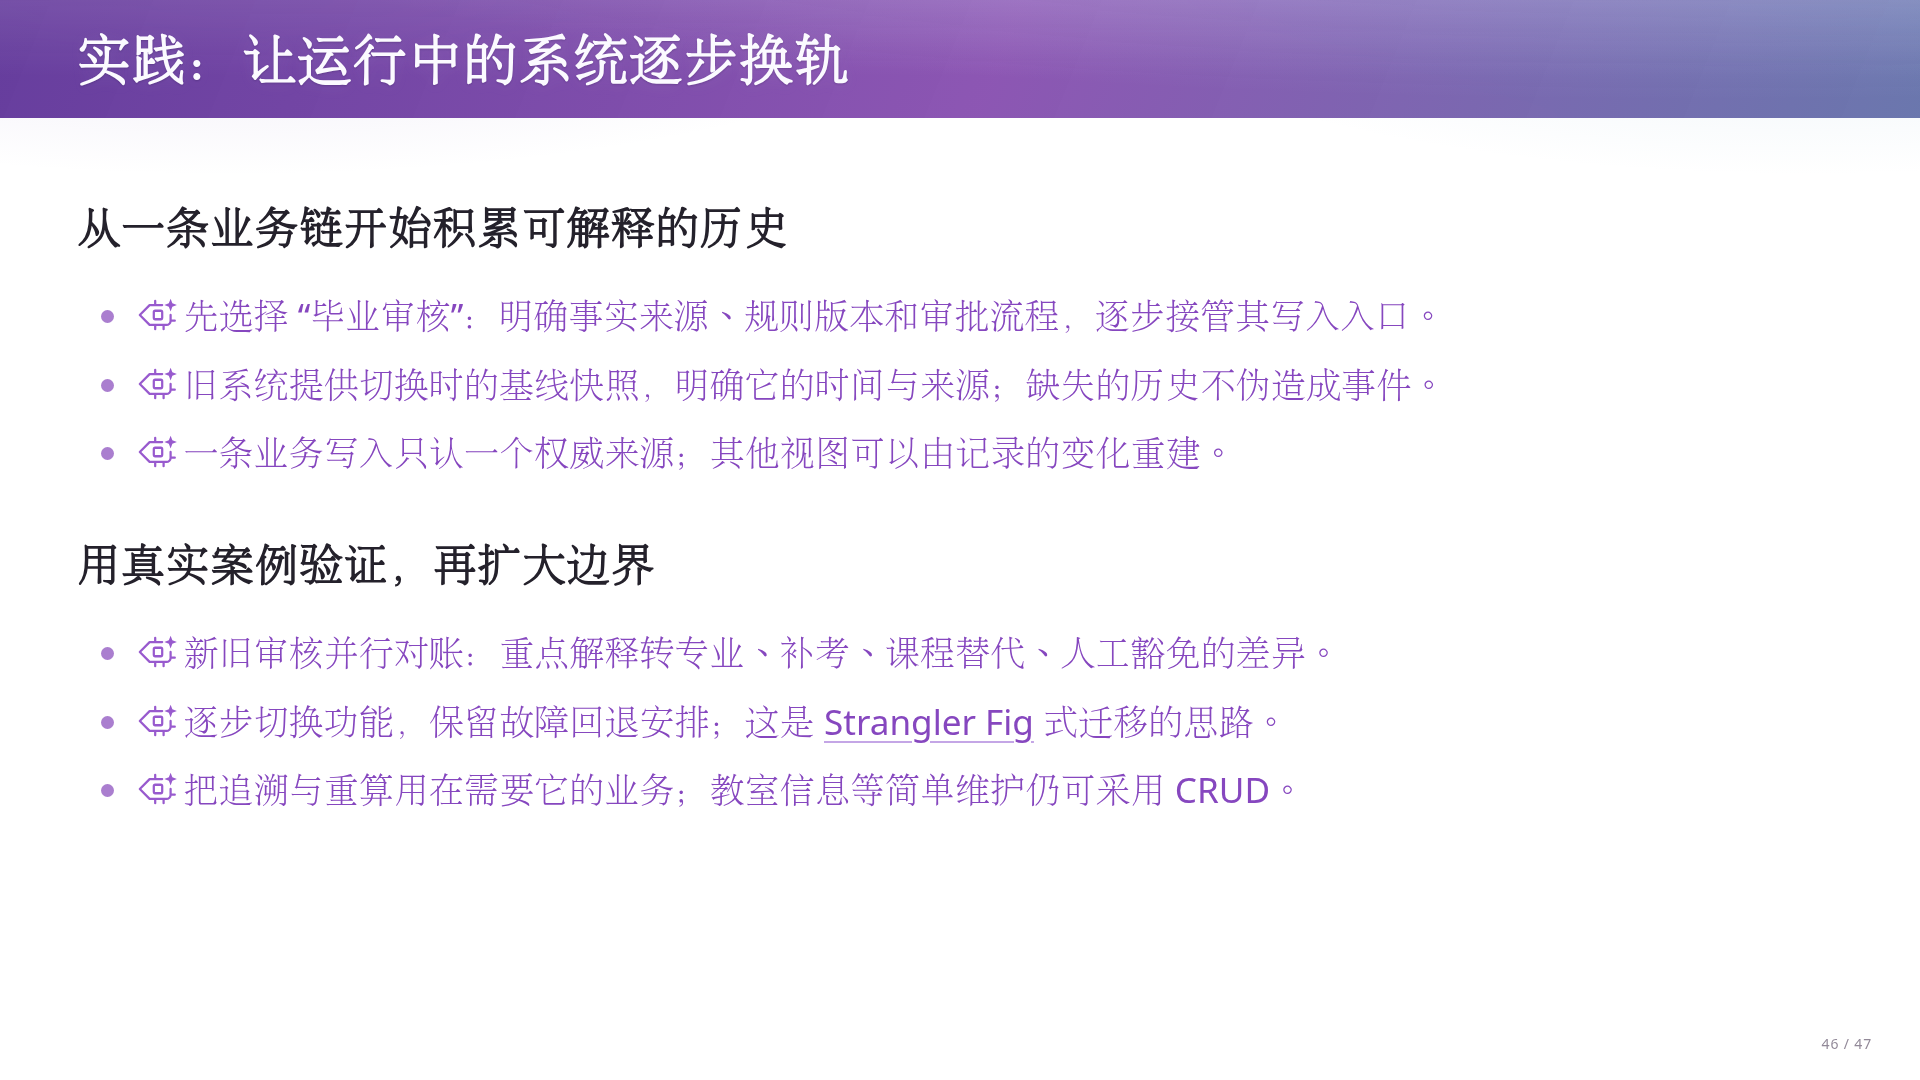
\includegraphics[width=\linewidth]{slides-images/slide-046.png}

\caption{实践落地：用绞杀者模式让运行中的旧系统逐步换轨（官方课件第 46 页）}

\end{figure}

让运行中的遗留系统逐步换轨，可以采用绞杀者模式（Strangler Fig Pattern，像绞杀榕逐步包裹老树一样，在旧系统外围按业务链逐步构建新模块并接管流量，直至安全替换旧系统的迁移策略）。第一步，先选择一条最需要可解释性的核心业务链——如“毕业审核”——开始积累可解释的历史：梳理清楚它的事实来源、规则版本和审批流程，并逐步接管该业务的权威写入入口。在切换时刻，由旧系统提供一份带有明确时间戳和来源说明的基线快照（Baseline Snapshot，迁移切入点上如实记录旧系统当前存量状态及来源元数据的初始基准记录）；对于旧系统中已经丢失的历史过程，绝不伪造成系统亲眼记录过的历史事件。同时坚守一条铁律：同一条业务写入只认一个权威来源，其他查询视图均可由记录下来的状态变化重建。第二步，用真实历史案例验证后再扩大边界：让新旧两套毕业审核逻辑并行运行与对账，重点比对并解释转专业、补考、课程替代、人工豁免等复杂边缘案例中的结论差异；在逐步切换功能的同时保留故障回退安排。此外，架构改造应当讲究投入产出比：把高成本的依赖追溯与规则重算精准用在毕业审核、学分认定等确实需要解释依据的业务上，而像教室基本信息维护这类简单场景，继续保留直接的 CRUD 即可。

这种渐进式换轨策略之所以稳妥，是因为它承认了历史遗产的客观限制：不强求把旧数据库里含义不明的存量状态硬编造出虚假的审批事件，而是以明确标注来源的基线快照作为诚实的分水岭，保证切换点之后的每一笔新业务都拥有完整的事件、依赖与规则版本记录。当我们在十行、两千行与五十万行三个尺度上完整经历了架构演进的思考后，最后让我们回到生成式 AI 时代的起点，审视架构概念在人机协作中的决定性力量。

\subsection{全篇升华：几个字的架构提示，改变整个系统的走向}

回顾本讲开篇的问题：当 Agentic AI 能够在几分钟内根据需求说明书生成出看似功能完备的教务系统原型时，人类软件工程师不可替代的价值究竟在哪里？对比相同的教务需求在三种不同架构指令下的演化路径，我们可以看清架构决策对系统长期走向的影响。

\begin{figure}[H]\centering

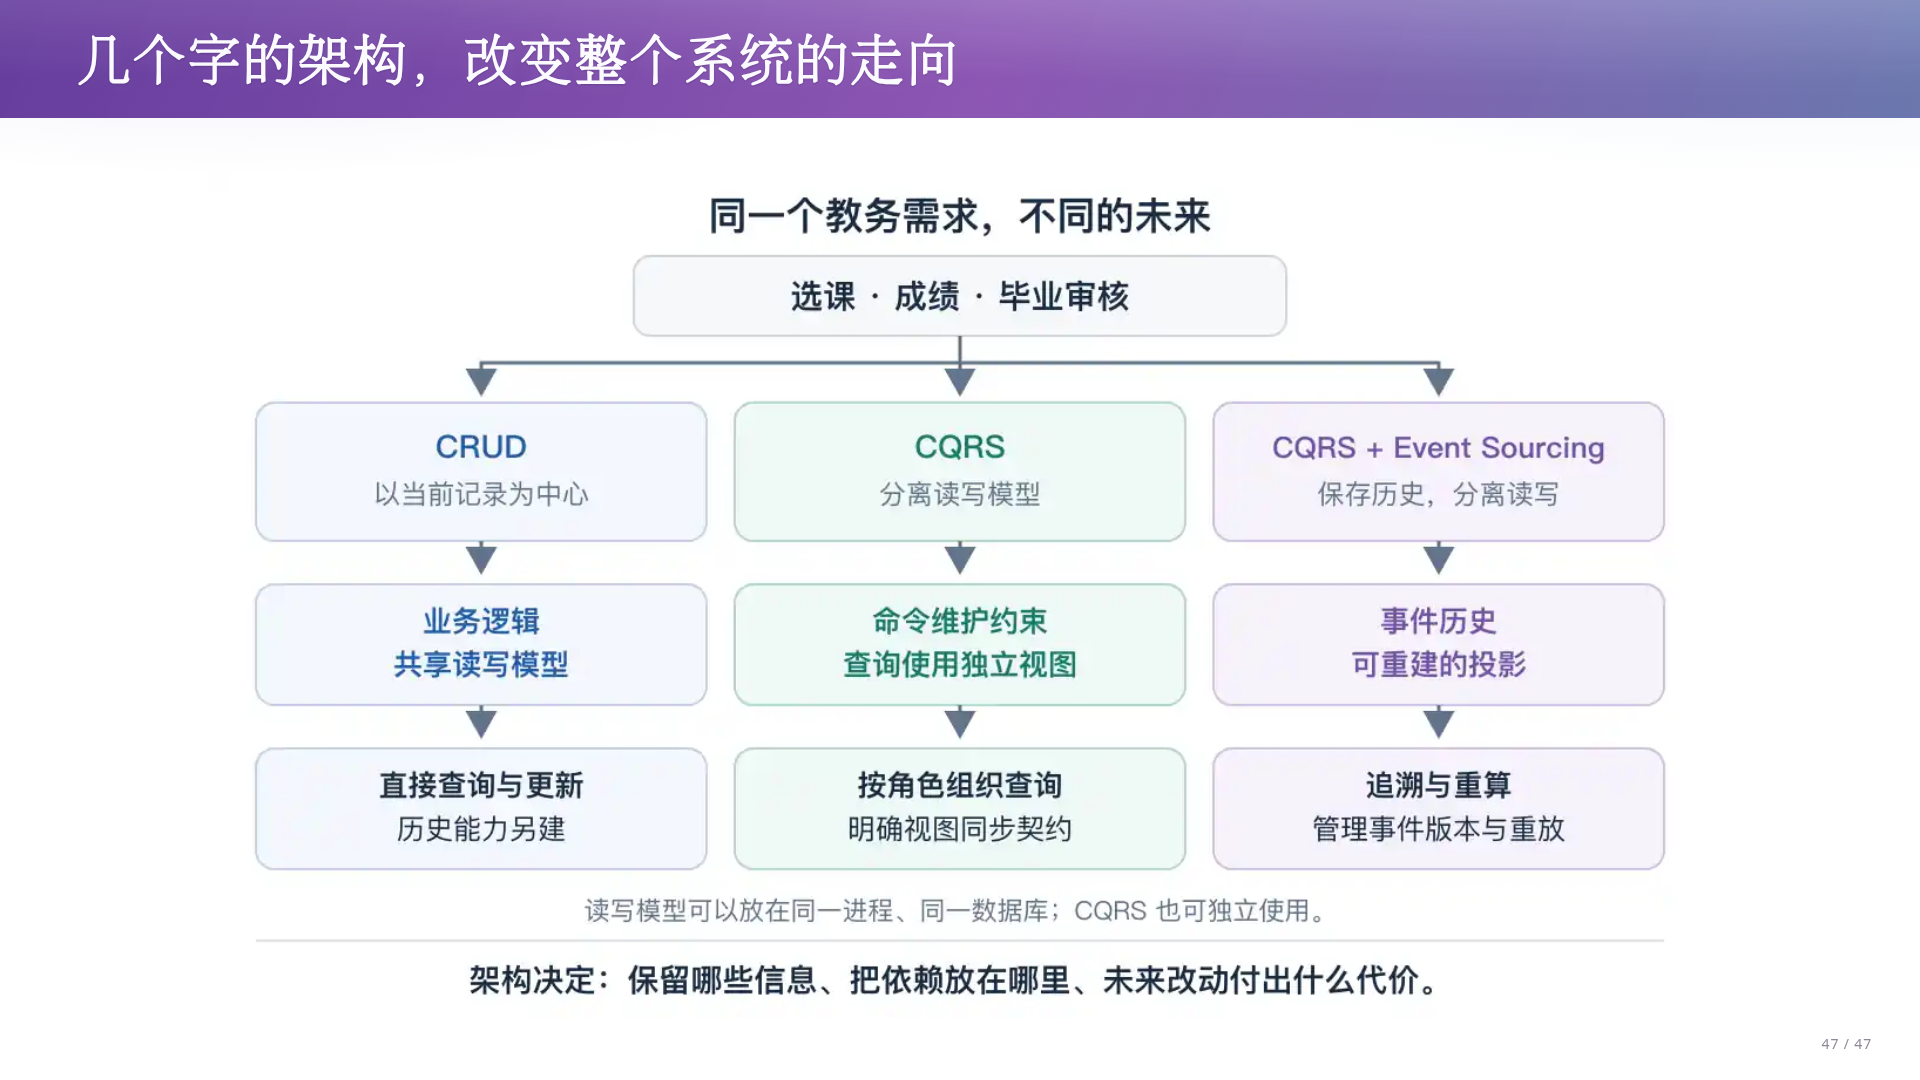
\includegraphics[width=\linewidth]{slides-images/slide-047.png}

\caption{全篇升华：几个字的架构提示，改变整个系统的走向（官方课件第 47 页）}

\end{figure}

通过“相同教务需求在 CRUD、CQRS、CQRS 加 Event Sourcing 下的不同演化路径”对照图，我们可以收束全讲的主线。在生成式 AI 时代，如果我们在给 AI 的 Prompt 里什么架构约束都不提，它默认就会沿着最常见的無历史状态表路径，生成出一套把业务逻辑挤在几个大文件里、直接原地覆写当前数据库状态的系统；随着时间推移，需求变更与线下特例会将其拖入难以解释的数据泥潭。相反，当我们在 Prompt 中明确给出“采用 CQRS”或“采用 CQRS + Event Sourcing”，并进一步约定规则版本、输入依赖与并发边界时，AI 就会生成出结构截然不同的系统：写模型集中守护业务不变量，读模型按角色分离出定制视图，而事件流与显式保存的规则版本及输入依据则让历史决定可追溯、可解释。

课堂提示我们，给 AI 增加这几个字看似轻巧，但这几个字之所以能发挥四两拨千斤的杠杆作用，前提是工程师自己真正理解它们背后的第一性原理：究竟由谁来维护业务约束？哪些历史信息与依赖关系必须作为一等公民保留？当需求语义发生漂移时，变化会沿着什么路径传播？代码生成得越便宜、越迅速，我们就越值得在这些数量极少、却从根本上决定软件品味与系统能走多远的架构决定上投入深思。

\begin{importantbox}{DDD、CQRS 与事件溯源的正交组合与模块化单体}

在架构设计中，DDD、CQRS 与事件溯源（Event Sourcing）解决的是三个不同维度的问题：DDD 负责划分业务语义与限界上下文边界，CQRS 负责分离命令写入与查询读取的模型职责，事件溯源负责以追加事件序列的方式保存和重建状态历史。三者彼此独立、正交，可按业务复杂度单独采用或按需组合，绝不强制捆绑，也绝不强制拆分为分布式微服务——它们完全可以在同一个进程、同一个数据库的模块化单体中高效落地。

\end{importantbox}

\begin{knowledgebox}{双时态历史：区分现实生效时间与系统获知时间}

现实世界的业务审批往往先于信息系统的录入动作。双时态历史通过同时保存“现实业务生效时间”（Valid Time）与“系统获知录入时间”（Transaction Time），彻底消除了跨期补录带来的逻辑悖论。面对“6月1日生效、6月3日录入”的豁免批件，系统既能基于生效时间确认学生在6月2日已具备豁免资格，又能基于录入时间复现6月2日当天系统因尚未获知该事实而拒绝毕业申请的真实历史原因。

\end{knowledgebox}

\begin{warningbox}{遗留系统换轨切忌伪造缺失历史与滥用重算架构}

对运行中的旧系统做渐进式迁移时，有两个常见误区必须规避：第一，严禁把旧数据库中已经丢失演变过程的存量状态伪装成系统亲眼记录过的历史事件，旧数据只能作为标明切换时间与来源的基线快照（Baseline Snapshot）接入新系统；第二，事件溯源、依赖追踪与规则重算具有显著的建模与维护成本，应聚焦于毕业审核、学分认定等强解释性核心链路，切勿滥用到教室信息维护等普通 CRUD 场景。

\end{warningbox}

\par\needspace{5\baselineskip}\textbf{术语消化：复杂业务系统核心架构模式与演化机制对照表}

\begin{center}\small\begin{tabularx}{\linewidth}{YYY}

\toprule

术语 & 解决的问题 & 机制与课程关系\\\midrule

CQRS（命令与查询职责分离） & 单一数据模型难以同时兼顾严密的写端业务校验与多角色异构的高效查询 & 将检查资格、容量与冲突的写模型（Command）与预计算、适当冗余的读模型（Query）分开设计，可共享同一进程与数据库\\[3pt]

DDD 限界上下文（Bounded Context） & 全局共享单一“超级模型”导致选课、财务、毕业审核的业务语义混杂与字段污染 & 在明确边界内维持统一语言，让不同业务板块各自维护专属的“学生”状态与规则，通过明确契约传递信息\\[3pt]

双时态历史（Bitemporal History） & 线下审批生效与线上录入存在时间差时，单一时间戳无法同时解释业务有效性与系统历史行为 & 分别记录“现实业务发生/生效时间”与“系统得知/录入时间”，支撑跨期审计与历史状态复现\\[3pt]

基线快照（Baseline Snapshot） & 遗留系统迁移时历史过程已丢失，直接编造虚假历史事件会破坏审计真实性 & 在绞杀者模式换轨切入点如实冻结旧系统存量状态并标明时间与来源，作为后续真实事件流的合法起点\\[3pt]

模块化单体（Modular Monolith） & 过早拆分分布式微服务带来高昂的跨网调用与运维成本，却未理清核心业务边界 & 在同一程序和部署单元内按信息隐藏原则隔离培养方案、课程替代等易变决策，理清数据归属与接口契约\\[3pt]

\bottomrule\end{tabularx}\end{center}

\begin{lstlisting}[basicstyle={\ttfamily\small\linespread{1}\selectfont},captionpos=t,caption={带输入依赖、规则版本与双时态时间戳的毕业审核及乐观并发选课伪代码}]
from dataclasses import dataclass
from datetime import datetime
from typing import List, Optional

@dataclass(frozen=True)
class InputRef:
    record_id: str
    version: int

@dataclass(frozen=True)
class BitemporalExemption:
    exemption_id: str
    student_id: str
    rule_item: str
    effective_at: datetime   # 现实业务生效时间 (如 6月1日)
    recorded_at: datetime    # 系统获知录入时间 (如 6月3日)
    approver: str
    reason: str

@dataclass(frozen=True)
class GraduationAuditDecision:
    audit_id: str
    student_id: str
    plan_rule_version: str          # 适用的培养方案规则版本
    input_dependencies: List[InputRef]  # 显式记录依赖的成绩/替代/豁免记录及版本
    can_graduate: bool
    approval_basis: str
    decided_at: datetime

def is_exemption_active(ex: BitemporalExemption, business_time: datetime, system_known_before: Optional[datetime] = None) -> bool:
    """双时态查询：区分'当时业务上是否生效'与'当时系统是否已知晓'"""
    if system_known_before is not None and ex.recorded_at > system_known_before:
        return False
    return ex.effective_at <= business_time

def enroll_last_seat_atomic(event_store, course_id: str, student_id: str) -> bool:
    """写模型命令处理：通过事件流乐观并发控制保证容量检查与占位的原子性"""
    stream_id = f"course-capacity-{course_id}"
    events, expected_version = event_store.read_stream(stream_id)

    capacity, enrolled_students = project_capacity_state(events)
    if student_id in enrolled_students or len(enrolled_students) >= capacity:
        return False

    new_event = {"type": "SeatReserved", "course_id": course_id, "student_id": student_id}
    # 追加时原子校验 expected_version，若并发冲突则抛出异常由上层重新加载并判断
    return event_store.append_to_stream(stream_id, [new_event], expected_version=expected_version)
\end{lstlisting}

该伪代码展示了本章落地的两个核心机制：一是 GraduationAuditDecision 与 BitemporalExemption 结构，将培养方案规则版本、输入记录依赖（ID 与版本）以及现实生效时间（effective\_at）和系统录入时间（recorded\_at）显式建模，使 \texttt{is\_exemption\_active} 能准确回答“6月2日豁免是否已生效”与“截至6月2日系统所知状态下为何拒绝毕业”；二是 \texttt{enroll\_last\_seat\_atomic} 函数，演示了在事件存储上处理最后名额争抢时，写端通过校验事件流 \texttt{expected\_version} 实现原子性的容量检查与占位。

\needspace{7\baselineskip}\subsection{本章小结}

本章阐述了如何通过 CQRS 分离维护业务不变量的写模型与面向多角色优化的\textbf{读模型}，并利用 DDD 的统一语言与\textbf{限界上下文}划清选课、财务与毕业审核的语义边界。

在工程落地上，通过为审核结论绑定输入依赖、规则版本与双时态时间戳，结合模块化单体与绞杀者模式（基于基线快照与新旧并行对账），系统得以在稳妥换轨的同时从容应对未来的需求变化。

\needspace{8\baselineskip}\section{总结与延伸}

回顾本讲，软件架构的本质并非盲目堆砌微服务或复杂中间件，而是“如何看待和表示问题”的选择——即把复杂性安放在何处，以及\textbf{如何用清晰的边界隔离未来的变化}。

\begin{itemize}
\item 在\textbf{十行代码}的尺度上，非递归汉诺塔在限定 \texttt{1 <= n < 64} 且总步数仍为 \(2^n - 1\) 步的前提下，既可以用二进制位运算表达数学规律，也可以用任务栈分解子问题，或是基于小步操作语义构造带程序计数器的抽象机器；不同表示直接决定了认知负担与应对规则改变的能力。

\item 在\textbf{两千行代码}的尺度上，面对 Excel 长公式极度脆弱的困境，课堂设想通过“跳出问题看问题”引入编译器架构：将用户输入保留为符号、将受输入影响的分支表示为条件选择节点，通过中间表示（IR）解耦算法构造、单元格布局与目标版本能力；同时，由于 Python 与 Excel 双后端共用同一份 IR 可能共享算法错误，还需固定编码参数并借助独立实现或独立解码器完成核验。

\item 在\textbf{五十万行教务系统}的尺度上，针对虚构的 160 学分转专业培养方案、未查明具体代码根因却引发全局 500 瘫痪的 \texttt{-1} 缺课记录，以及“系改院”带来的组织身份与历史归属两难，我们看到经典 CRUD 架构将“历史事实、适用规则与决策结果”压缩为无历史快照的局限。

\item 为此，工程实践中可按需独立或组合采用 DDD（划分限界上下文与统一语言）、CQRS（分离维护约束的写模型与定制优化的读模型，无需强制拆分微服务）与事件溯源（把状态变化保存为事件序列）。在重放历史时，必须严格区分“\textbf{还原历史事实}”与“\textbf{按新规则重算}”，显式记录规则版本、输入依赖与双时态时间，并隔离发短信、扣费等外部副作用；对运行中的遗留系统，则可采用绞杀榕模式从单条业务链渐进换轨。

\end{itemize}
承上启下，本讲将上一讲的“数据依赖图”落地为具体的架构分解与状态建模机制，而给 AI 提示词中增加几个字的架构概念之所以能彻底改变系统走向，正源于背后的第一性原理思考；这也为下一讲继续探讨需求与架构的深层工程实践奠定了基础。

\subsection{学习练习}

用下面的延伸练习检查自己能否应用本讲方法。

\needspace{6\baselineskip}\subsubsection*{练习 1：非递归算法的多重架构表示与变体演进}

请针对经典的汉诺塔问题（限定 1 <= n < 64），用 C 或 Python 分别实现“二进制数学规律”“显式任务栈”和“带 pc 的抽象机器（模拟栈帧）”三种非递归版本。随后引入一项需求变更：新增规则“禁止任何盘子直接从 A 柱移动到 C 柱（或从 C 直接到 A），每次移动必须经过中间的 B 柱”，请尝试在三种表示下分别修改代码以适应该变更，并撰写简短对比报告，分析哪种表示在规则改变时的修改边界最清晰。

\par\needspace{4\baselineskip}\textbf{验收标准：}

\begin{enumerate}
\item 三个基础版本在 1 <= n <= 10 时输出步数均为 2\textasciicircum{}n - 1 且移动序列完全一致，位运算使用 64 位无符号整数且无溢出；

\item 至少在“任务栈”或“抽象机器”版本上成功实现经过中间柱的新规则（总步数为 3\textasciicircum{}n - 1），并准确说明为何原二进制数学规律在新规则下直接失效。
\end{enumerate}

\needspace{6\baselineskip}\subsubsection*{练习 2：微型表格公式编译器的中间表示（IR）与双后端核验设计}

设想需要在电子表格中根据动态输入的字符串计算其 8 位校验和或简单哈希并展示为二进制位格。请用 Python 设计一套小型计算图 IR（包含符号输入 Input、常量 Const、按位异或 BitXor、算术运算及条件选择 Select 节点），并编写生成器将该 IR 分别翻译为可执行的 Python 函数与目标表格公式字符串（支持配置起始单元格偏移量与是否使用 LET 函数）。

\par\needspace{4\baselineskip}\textbf{验收标准：}

\begin{enumerate}
\item 用户输入在构图阶段严格保留为 Input 符号节点而非硬编码求值，与输入无关的计算在生成时完成常量折叠；

\item 修改布局偏移配置时无需改动算法构图代码即可重新生成正确引用的公式；

\item 编写验证脚本，对多组测试输入不仅对比 Python 后端与表格公式求值结果，还调用一个独立编写的参考函数进行交叉核验。
\end{enumerate}

\needspace{6\baselineskip}\subsubsection*{练习 3：教务毕业审核模块的命令查询分离（CQRS）与可解释历史建模}

针对本讲虚构的转专业培养方案（含课程替代、缓考暂选、成绩更正与线下特批“视为满足”），在一个单进程模块化程序中设计毕业审核领域模型：采用事件流记录选课、成绩登记、替代审批与人工豁免事实，实现写模型校验与读模型投影，并支持“恢复历史决定”与“按新版本培养方案重算”两种重放模式。

\par\needspace{4\baselineskip}\textbf{验收标准：}

\begin{enumerate}
\item 每次毕业审核结论必须显式保存所依赖的输入记录标识/版本、规则版本、审批依据以及双时态时间（业务生效时间与系统录入时间）；

\item 模拟一次历史成绩更正和一次培养方案规则升级，程序能准确列出受影响的历史审核记录，且按新规则重算不会自动抹除已发布的“授予学位”历史事实；

\item 重放历史事件重建读视图时，通过接口隔离机制确保通知发送等外部副作用函数被调用的次数为 0。
\end{enumerate}

\subsection{拓展阅读}

下面列出本讲的原始讲义、课件和相关项目，便于回看案例、查阅代码并继续实践。

\begin{itemize}

\item 官方讲义：\url{https://jyywiki.cn/GSE/2026/lect6.md}

\item 官方课件：\url{https://jyywiki.cn/GSE/2026/slides6.html}

\item 社区字幕校订稿（固定版本）：\url{https://github.com/NinZeige/NJU-2026-GSE-Captions/tree/0456f3a46fd5fa2f2a86123e02b7ed48696adacb}

\item 原课程许可 CC BY-NC 4.0：\url{https://creativecommons.org/licenses/by-nc/4.0/}

\item 上一讲：软件工程导论与形式化规约（lect5.md）：\url{https://jyywiki.cn/GSE/2026/lect5.md}

\item Dilemmas in a General Theory of Planning (Wicked Problems, Rittel \& Webber, 1973)：\url{https://doi.org/10.1007/BF01405730}

\item No Silver Bullet—Essence and Accidents of Software Engineering (Brooks, 1987)：\url{https://cgi.csc.liv.ac.uk/~coopes/comp319/2016/papers/NoSilverBullet-Brooks1987.htm}

\item On the Criteria To Be Used in Decomposing Systems into Modules (Parnas, 1972)：\url{https://ckrybus.com/static/papers/decomposing_systems_into_modules_1972.pdf}

\item Representations in Distributed Cognitive Tasks (Zhang \& Norman, 1994)：\url{https://pages.ucsd.edu/~scoulson/203/zhang.pdf}

\item Nayuki QR Code Generator (GitHub Repository)：\url{https://github.com/nayuki/QR-Code-generator}

\item Excel performance: Improving calculation performance (Microsoft Learn)：\url{https://learn.microsoft.com/en-us/office/vba/excel/concepts/excel-performance/excel-improving-calculation-performance}

\item LET function (Microsoft Support)：\url{https://support.microsoft.com/en-us/excel/functions/let-function}

\item 南大没系啦（微信公众号文章）：\url{https://mp.weixin.qq.com/s/ibm6hFMc_JaMOWlqg7RF7A}

\item Event Sourcing (Martin Fowler)：\url{https://martinfowler.com/eaaDev/EventSourcing.html}

\item Event Sourcing pattern (Microsoft Azure Architecture Center)：\url{https://learn.microsoft.com/en-us/azure/architecture/patterns/event-sourcing}

\item CQRS (Martin Fowler)：\url{https://martinfowler.com/bliki/CQRS.html}

\item CQRS pattern (Microsoft Azure Architecture Center)：\url{https://learn.microsoft.com/en-us/azure/architecture/patterns/cqrs}

\item BoundedContext (Martin Fowler)：\url{https://martinfowler.com/bliki/BoundedContext.html}

\item Domain-Driven Design Reference (Eric Evans)：\url{https://www.domainlanguage.com/wp-content/uploads/2016/05/DDD_Reference_2015-03.pdf}

\item Bitemporal History (Martin Fowler)：\url{https://martinfowler.com/articles/bitemporal-history.html}

\item Provenance in Databases: Why, How, and Where (arXiv:0708.2173)：\url{https://arxiv.org/abs/0708.2173}

\item Strangler Fig Application (Martin Fowler)：\url{https://martinfowler.com/bliki/StranglerFigApplication.html}

\end{itemize}

\end{document}
